\documentclass[12pt,a4paper]{book}
\usepackage{lmodern}
\usepackage{amssymb,amsmath}
\usepackage{ifxetex,ifluatex}
\usepackage{fixltx2e} % provides \textsubscript
\ifnum 0\ifxetex 1\fi\ifluatex 1\fi=0 % if pdftex
  \usepackage[T1]{fontenc}
  \usepackage[utf8]{inputenc}
\else % if luatex or xelatex
  \ifxetex
    \usepackage{mathspec}
  \else
    \usepackage{fontspec}
  \fi
  \defaultfontfeatures{Ligatures=TeX,Scale=MatchLowercase}
\fi
% use upquote if available, for straight quotes in verbatim environments
\IfFileExists{upquote.sty}{\usepackage{upquote}}{}
% use microtype if available
\IfFileExists{microtype.sty}{%
\usepackage{microtype}
\UseMicrotypeSet[protrusion]{basicmath} % disable protrusion for tt fonts
}{}
\usepackage[margin=2cm]{geometry}
\usepackage{hyperref}
\PassOptionsToPackage{usenames,dvipsnames}{color} % color is loaded by hyperref
\hypersetup{unicode=true,
            pdftitle={Notes on the design of a simple spatial sampling method (S3M) for assessing coverage of health and nutrition programmes in Liberia},
            pdfauthor={Valid International},
            colorlinks=true,
            linkcolor=blue,
            citecolor=blue,
            urlcolor=blue,
            breaklinks=true}
\urlstyle{same}  % don't use monospace font for urls
\usepackage{natbib}
\bibliographystyle{apalike}
\usepackage{longtable,booktabs}
\usepackage{graphicx,grffile}
\makeatletter
\def\maxwidth{\ifdim\Gin@nat@width>\linewidth\linewidth\else\Gin@nat@width\fi}
\def\maxheight{\ifdim\Gin@nat@height>\textheight\textheight\else\Gin@nat@height\fi}
\makeatother
% Scale images if necessary, so that they will not overflow the page
% margins by default, and it is still possible to overwrite the defaults
% using explicit options in \includegraphics[width, height, ...]{}
\setkeys{Gin}{width=\maxwidth,height=\maxheight,keepaspectratio}
\IfFileExists{parskip.sty}{%
\usepackage{parskip}
}{% else
\setlength{\parindent}{0pt}
\setlength{\parskip}{6pt plus 2pt minus 1pt}
}
\setlength{\emergencystretch}{3em}  % prevent overfull lines
\providecommand{\tightlist}{%
  \setlength{\itemsep}{0pt}\setlength{\parskip}{0pt}}
\setcounter{secnumdepth}{5}
% Redefines (sub)paragraphs to behave more like sections
\ifx\paragraph\undefined\else
\let\oldparagraph\paragraph
\renewcommand{\paragraph}[1]{\oldparagraph{#1}\mbox{}}
\fi
\ifx\subparagraph\undefined\else
\let\oldsubparagraph\subparagraph
\renewcommand{\subparagraph}[1]{\oldsubparagraph{#1}\mbox{}}
\fi

%%% Use protect on footnotes to avoid problems with footnotes in titles
\let\rmarkdownfootnote\footnote%
\def\footnote{\protect\rmarkdownfootnote}

%%% Change title format to be more compact
\usepackage{titling}

% Create subtitle command for use in maketitle
\newcommand{\subtitle}[1]{
  \posttitle{
    \begin{center}\large#1\end{center}
    }
}

\setlength{\droptitle}{-2em}

  \title{Notes on the design of a simple spatial sampling method (S3M) for
assessing coverage of health and nutrition programmes in Liberia}
    \pretitle{\vspace{\droptitle}\centering\huge}
  \posttitle{\par}
    \author{Valid International}
    \preauthor{\centering\large\emph}
  \postauthor{\par}
      \predate{\centering\large\emph}
  \postdate{\par}
    \date{2018-08-27}

\usepackage{booktabs}
\usepackage[table]{xcolor}
\usepackage{color}
\usepackage{tcolorbox}
\usepackage{float}
\usepackage{setspace}
\usepackage{longtable}
%\usepackage{amsmath}
%\usepackage{mathtools}

\onehalfspacing

%\raggedbottom

\graphicspath{ {icons/} }

\newenvironment{rmdremind}
  {\begin{tcolorbox}[width=\textwidth, 
                     colback = {white}, 
                     title = {\textbf{Remember}}, 
                     colbacktitle = lightgray,
                     coltitle = black]
  \begin{includegraphics}[scale = 1]{remind.png}
  \begin{itemize}}
  {\end{itemize}
  \end{includegraphics}
  \end{tcolorbox}}

\newenvironment{rmdnote}
  {\begin{tcolorbox}[width=\textwidth, 
                     colback = {white}, 
                     title = {\textbf{Note}}, 
                     colbacktitle = lightgray,
                     coltitle = black]
  \begin{includegraphics}[scale = 1]{pencil.png}}
  {\end{includegraphics}
  \end{tcolorbox}}
  
\newenvironment{rmdcalc}
  {\begin{tcolorbox}[width=\textwidth, 
                     colback = {white}, 
                     title = {\textbf{Calculations}}, 
                     colbacktitle = lightgray,
                     coltitle = black]
  \begin{includegraphics}[scale = 2]{pencil.png}}
  {\end{includegraphics}
  \end{tcolorbox}}
  
\newenvironment{rmdexercise}
  {\begin{tcolorbox}[width=\textwidth, 
                     colback = {white}, 
                     title = {\textbf{Exercise}}, 
                     colbacktitle = lightgray,
                     coltitle = black]
  \begin{includegraphics}[scale = 1]{exercise.png}}
  {\end{includegraphics}
  \end{tcolorbox}}
  
\newenvironment{rmdbox}
  {\begin{tcolorbox}[width=\textwidth, 
                     colback = {white}, 
                     title = {\textbf{Exercise}}, 
                     colbacktitle = lightgray,
                     coltitle = black]
  \begin{includegraphics}[scale = 1]{pencil.png}}
  {\end{includegraphics}
  \end{tcolorbox}}
  
\newenvironment{rmdinfo}
  {\begin{tcolorbox}[width=\textwidth, 
                     colback = {white}, 
                     title = {\textbf{Info}}, 
                     colbacktitle = lightgray,
                     coltitle = black]
  \begin{includegraphics}[scale = 1]{info.png}}
  {\end{includegraphics}
  \end{tcolorbox}}  
  
\newenvironment{rmdwarning}
  {\begin{tcolorbox}[width=\textwidth, 
                     colback = {white}, 
                     title = {\textbf{Warning}}, 
                     colbacktitle = lightgray,
                     coltitle = black]
  \begin{includegraphics}[scale = 1]{warning.png}}
  {\end{includegraphics}
  \end{tcolorbox}}

\newenvironment{rmdcaution}
  {\begin{tcolorbox}[width=\textwidth, 
                     colback = {white}, 
                     title = {\textbf{Caution}}, 
                     colbacktitle = lightgray,
                     coltitle = black]
  \begin{includegraphics}[scale = 1]{warning.png}}
  {\end{includegraphics}
  \end{tcolorbox}}

\newenvironment{rmddownload}
  {\begin{tcolorbox}[width=\textwidth, 
                     colback = {white}, 
                     title = {\textbf{Download}}, 
                     colbacktitle = lightgray,
                     coltitle = black]
  \begin{includegraphics}[scale = 1]{download.png}}
  {\end{includegraphics}
  \end{tcolorbox}}

\usepackage{amsthm}
\newtheorem{theorem}{Theorem}[chapter]
\newtheorem{lemma}{Lemma}[chapter]
\theoremstyle{definition}
\newtheorem{definition}{Definition}[chapter]
\newtheorem{corollary}{Corollary}[chapter]
\newtheorem{proposition}{Proposition}[chapter]
\theoremstyle{definition}
\newtheorem{example}{Example}[chapter]
\theoremstyle{definition}
\newtheorem{exercise}{Exercise}[chapter]
\theoremstyle{remark}
\newtheorem*{remark}{Remark}
\newtheorem*{solution}{Solution}
\let\BeginKnitrBlock\begin \let\EndKnitrBlock\end
\begin{document}
\maketitle

{
\hypersetup{linkcolor=black}
\setcounter{tocdepth}{1}
\tableofcontents
}
\hypertarget{simple-spatial-sampling-method-s3m}{%
\chapter*{Simple Spatial Sampling Method
(S3M)}\label{simple-spatial-sampling-method-s3m}}
\addcontentsline{toc}{chapter}{Simple Spatial Sampling Method (S3M)}

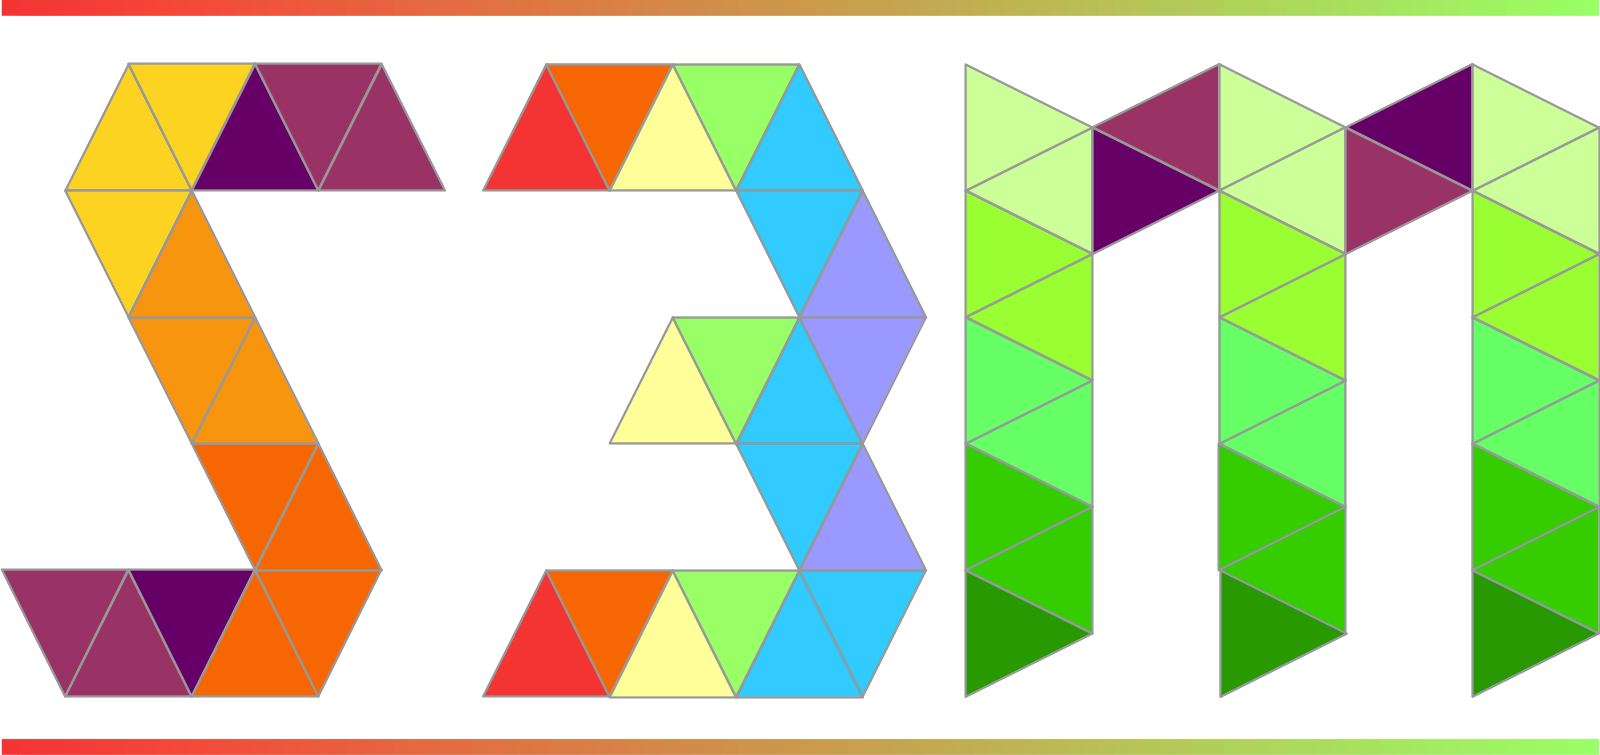
\includegraphics{figures/s3mlogo.png}

\hypertarget{introduction}{%
\chapter{Introduction}\label{introduction}}

The Simple Spatial Survey Method (S3M) was developed from the CSAS
coverage survey method as a response to the widespread adoption of
community management of acute malnutrition (CMAM) by ministries of
health. Large-scale programs need a large-scale survey method and S3M
was developed to meet that need.

S3M was designed to :

\begin{itemize}
\item
  Be simple enough for MoH, NGO, and UNO personnel without specialist
  statistical training to perform.
\item
  Provide a general survey method. S3M can be used to survey and map :

  \begin{itemize}
  \item
    Need for and coverage of selective-entry programs such as CMAM and
    TSFP as well as universal programs such as EPI, GMP, GFD (general
    ration), and ``blanket'' SFP over wide areas.
  \item
    Levels of indicators such as those for IYCF, WASH, and period
    prevalence / cumulative prevalence of ARI, fever, and diarrhoea over
    wide areas.
  \end{itemize}
\end{itemize}

This document concentrates on using S3M to assess the need for and
coverage of:

\begin{itemize}
\item
  Treatment of SAM in children aged between 6 and 59 months;
\item
  Vitamin A supplementation;
\item
  Micronutrient powder supplementation;
\item
  Ferrous sulphate-folic acid supplementation; and,
\item
  Infant and young child feeding counselling.
\end{itemize}

\hypertarget{sample}{%
\chapter{The survey sample}\label{sample}}

The survey method described here uses a two-stage sample:

\begin{itemize}
\item
  \textbf{First-stage:} We take an even (or near-even) spatial sample of
  communities from all of the communities in the survey area.
\item
  \textbf{Second-stage:} We take a sample of eligible individuals from
  each of the communities identified in the first stage of sampling.
\end{itemize}

Two-stage sampling is used in many survey methods. A typical example of
a survey method that uses a two-stage sample is the SMART method that is
commonly used for nutritional anthropometry surveys.

The main difference between the sample taken in S3M based surveys and in
SMART type surveys is that S3M based samples use a spatial sample in the
first stage whereas SMART type surveys use a proportional to population
size (PPS) sample.

The advantages of using a spatial first stage sample is that such a
sample allows us to identify where (and why) coverage is good, and where
(and why) coverage is poor. This information is essential to improving
program coverage and ensuring equitable access to services.

A spatial sample can be used to produce equivalent results to a
traditional proportional to population size (PPS) sample as is used in
(e.g.) SMART type surveys using a weighted analysis. This means that a
spatial sample can be made to act as a PPS sample. A PPS type sample
cannot, however, be made to act as a spatial sample.

\hypertarget{stage1}{%
\section{The first stage sample}\label{stage1}}

\hypertarget{step-1-find-a-map}{%
\subsection{Step 1: Find a map}\label{step-1-find-a-map}}

The first step in a S3M survey is to find a map of the survey area. A
map showing the locations of all towns and villages in the survey area
is essential. Try to find a map showing the locations of all towns and
villages in the survey area. You may need to update the map to take into
account migration and displacement.

For the coverage survey of 2 counties in Liberia, it will be practical
and useful to have:

\begin{itemize}
\tightlist
\item
  A small scale-map (a wide area map but with poor detail) of the entire
  survey area for each of the 2 counties. If the counties are contiguous
  (i.e., share borders with each other), the small scale map can be of
  the two counties together. This map does not need to show the location
  of all towns and villages in the survey area but it gives a general
  idea of where the 2 counties are located and main towns and locations
  and roads. Figure \ref{fig:smallScaleMap} is a small scale map of
  Liberia showing counties, roads and main towns and locations. Figure
  \ref{fig:smallScaleMapCounty} is a small scale map of two counties
  showing all the districts within the county, roads and main towns and
  locations.
\end{itemize}

\newpage

\begin{figure}[H]

{\centering 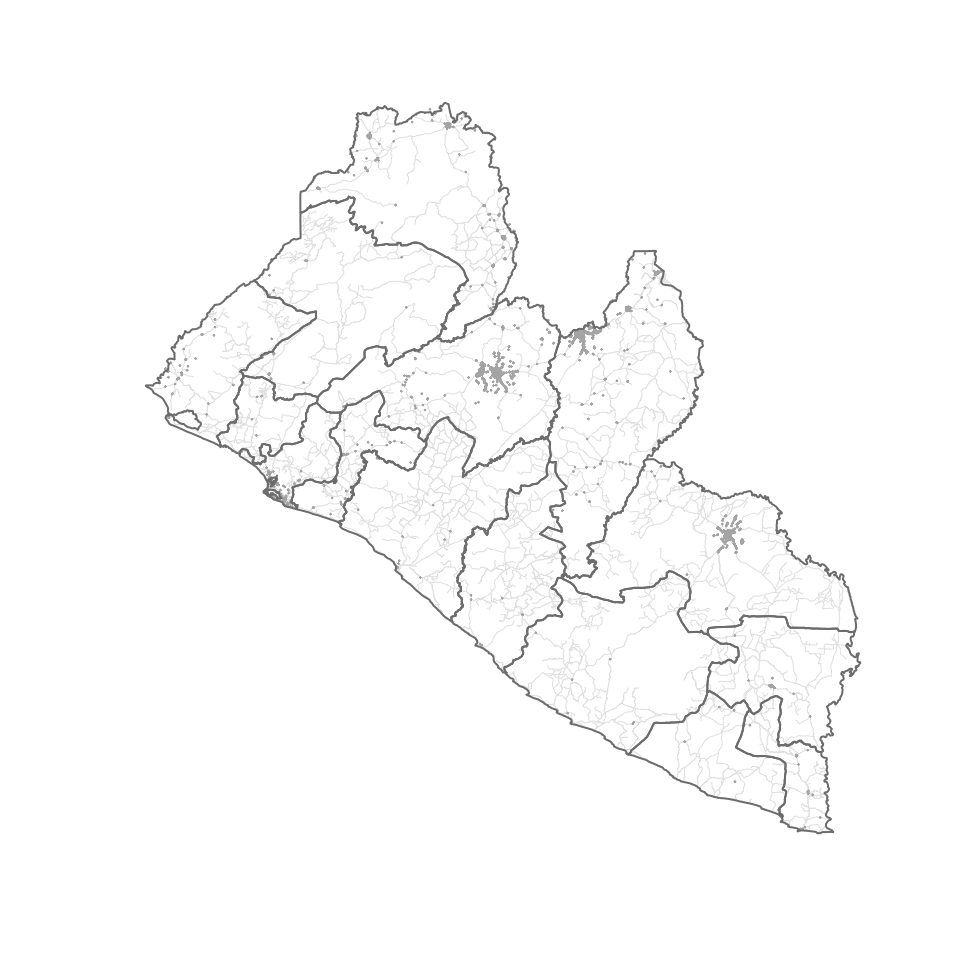
\includegraphics{figures/smallScaleMap-1} 

}

\caption{Small scale map of Liberia showing counties, roads and points of interest}\label{fig:smallScaleMap}
\end{figure}

\newpage

\begin{figure}[H]

{\centering 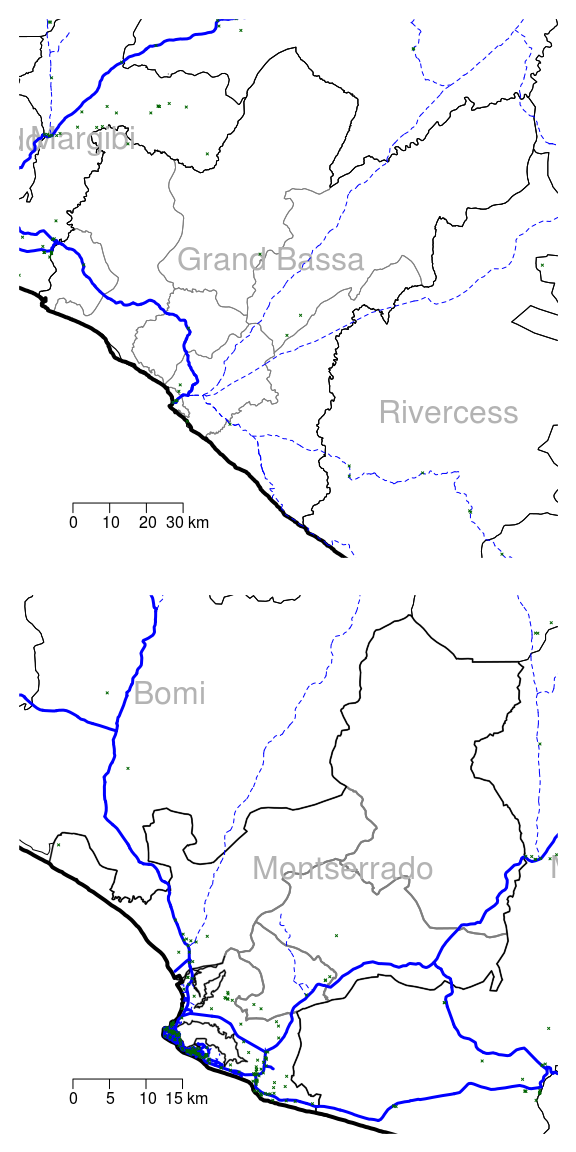
\includegraphics{figures/smallScaleMapCounty-1} 

}

\caption{Small scale map of Montserrado and Grand Bassa in Liberia showing all districts, roads and points of interest}\label{fig:smallScaleMapCounty}
\end{figure}

\newpage

\begin{itemize}
\tightlist
\item
  A collection of larger scale maps (a small area map but with good
  detail) of each of the selected counties and each of the districts
  within those counties in Liberia. Figure
  \ref{fig:largeScaleMapCounty1} is a large scale map of Montserrado
  county showing all districts, roads and all settlements. Figure
  \ref{fig:largeScaleMapDistricts1} is a collection of large scale maps
  of each of the districts of Montserrado country showing all roads and
  all settlements.
\end{itemize}

~

\begin{figure}[H]

{\centering 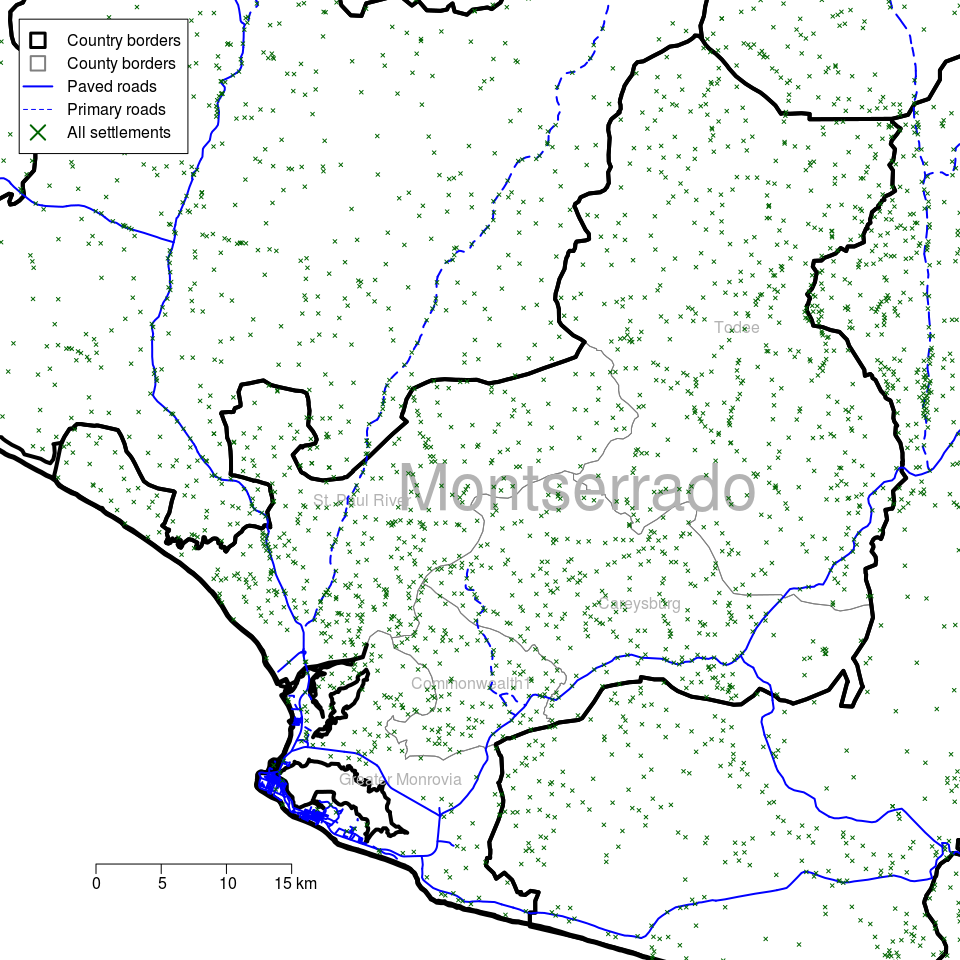
\includegraphics{figures/largeScaleMapCounty1-1} 

}

\caption{Large scale map of Montserrado county in Liberia showing all districts, roads and all settlements (towns, villages)}\label{fig:largeScaleMapCounty1}
\end{figure}

\newpage

\begin{figure}[H]

{\centering 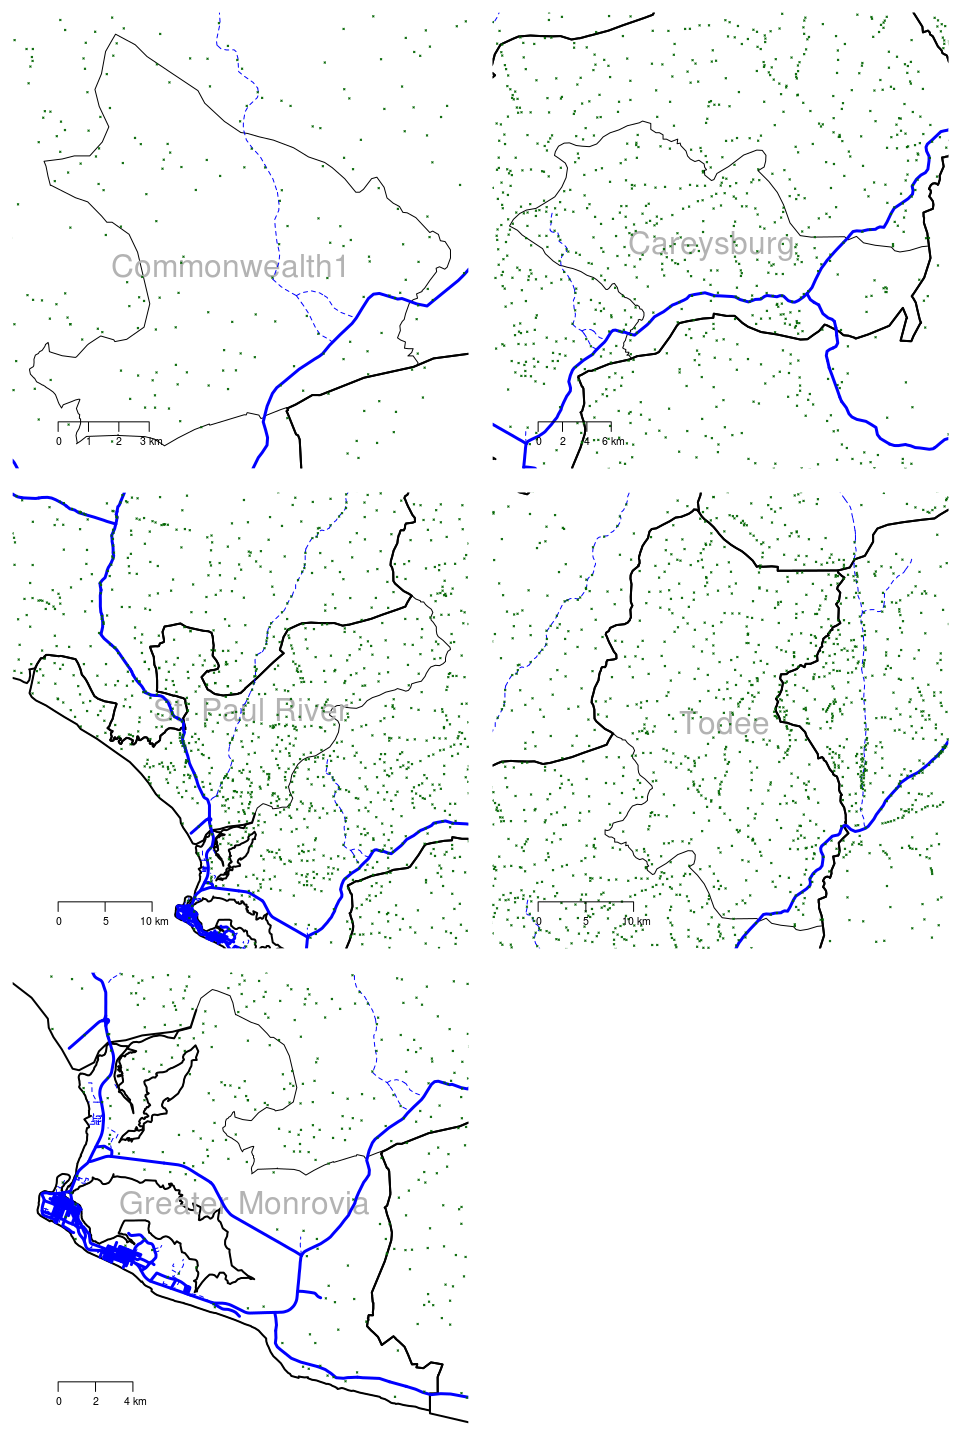
\includegraphics{figures/largeScaleMapDistricts1-1} 

}

\caption{Large scale maps of 5 districts of Montserrado county in Liberia showing roads and all settlements (towns, villages)}\label{fig:largeScaleMapDistricts1}
\end{figure}

\newpage

\begin{figure}[H]

{\centering 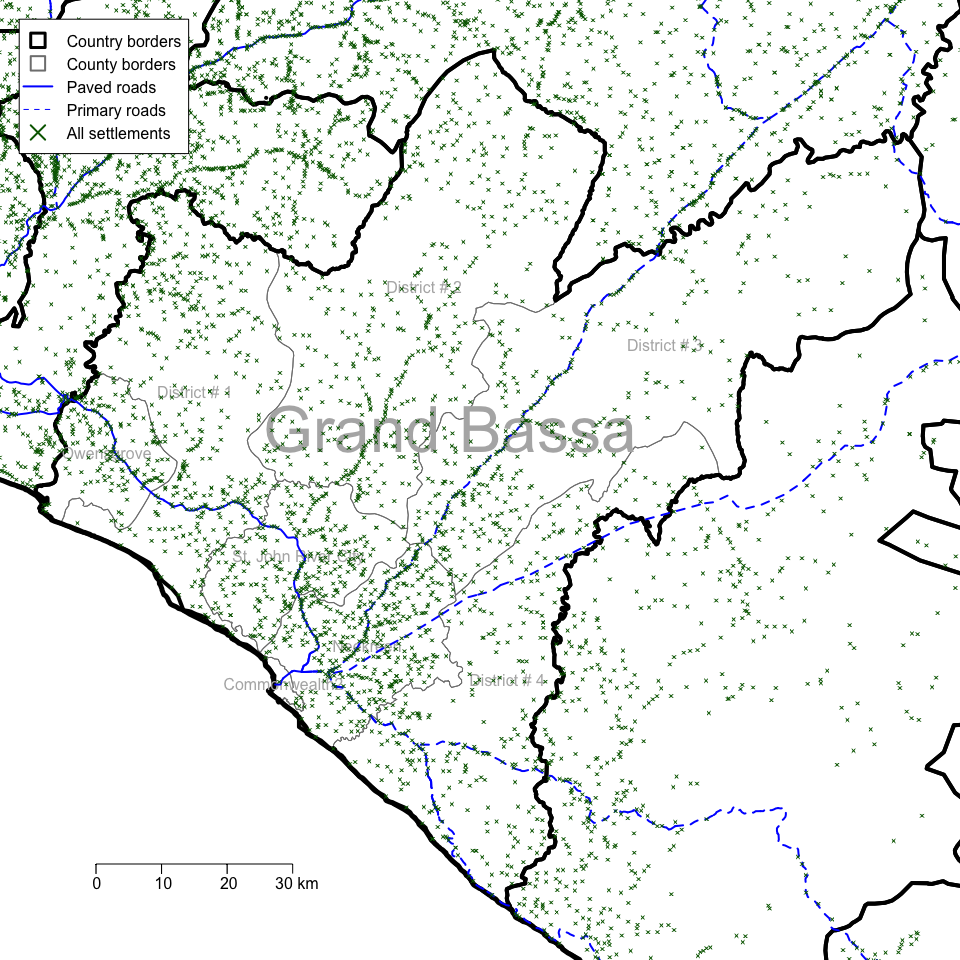
\includegraphics{figures/largeScaleMapCounty2-1} 

}

\caption{Large scale map of Grand Bassa county in Liberia showing all districts, roads and all settlements (towns, villages)}\label{fig:largeScaleMapCounty2}
\end{figure}

\newpage

\begin{figure}[H]

{\centering 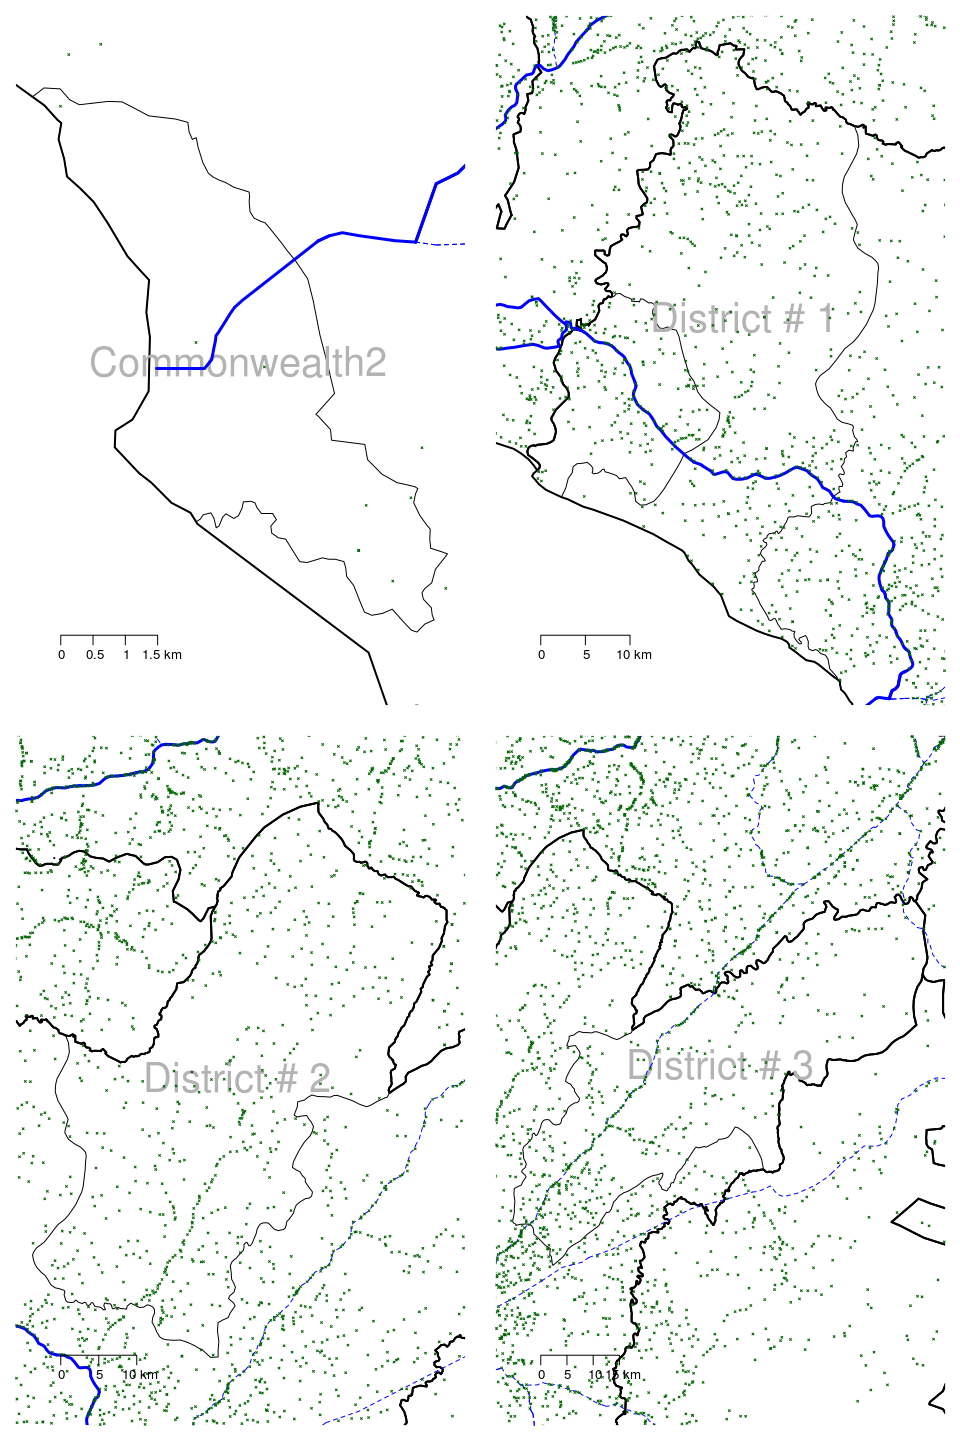
\includegraphics{figures/largeScaleMapDistricts2-1} 

}

\caption{Large scale maps of 8 districts of Grand Bassa county in Liberia showing roads and all settlements (towns, villages)}\label{fig:largeScaleMapDistricts2}
\end{figure}

\newpage

\begin{figure}[H]

{\centering 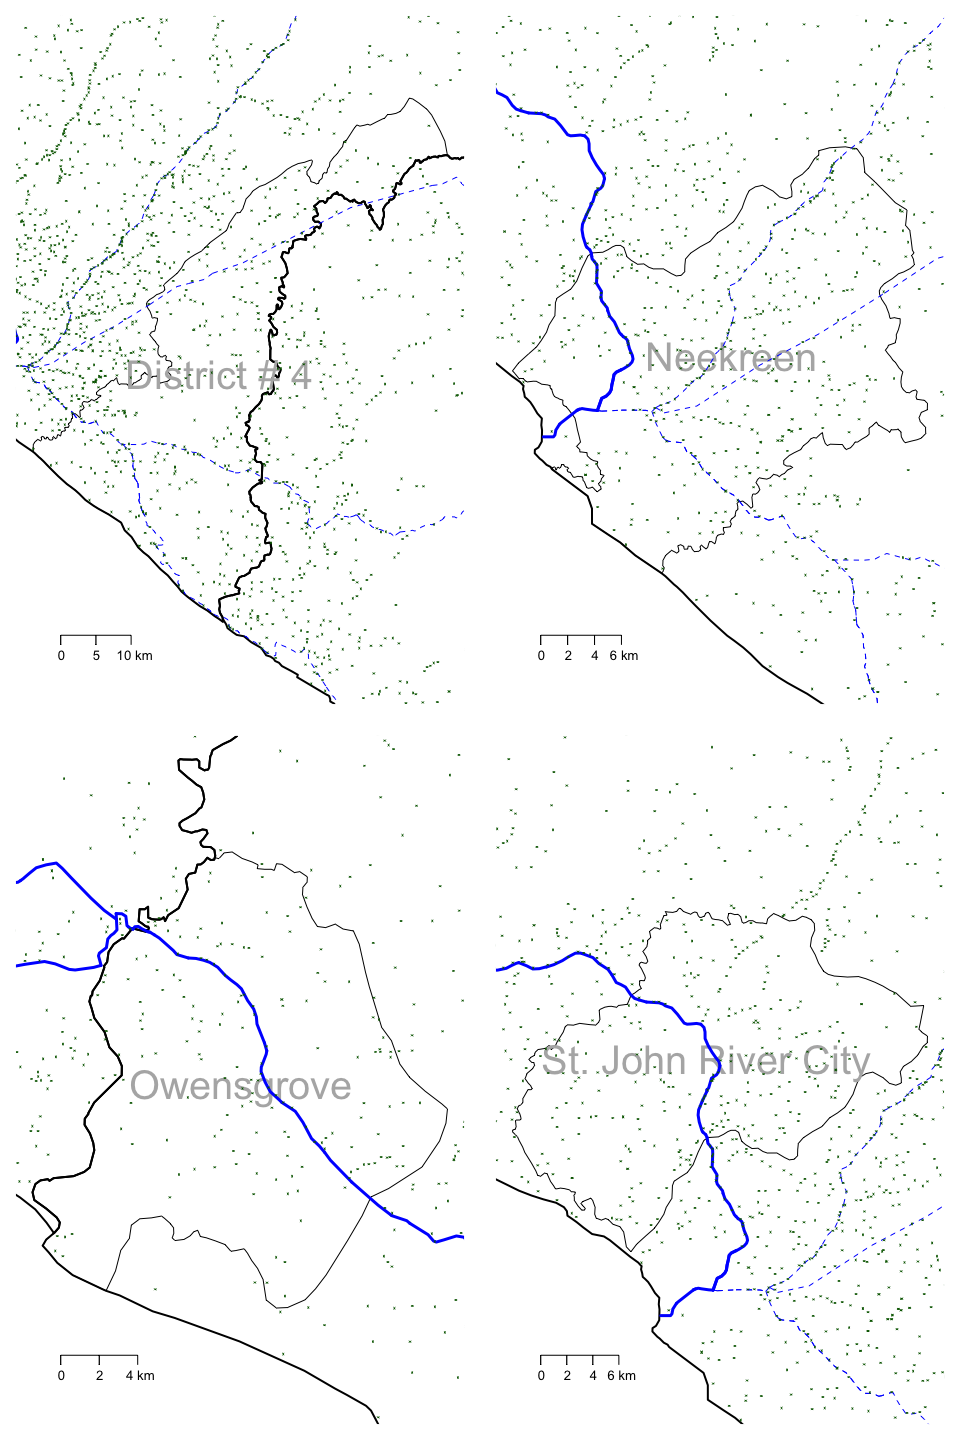
\includegraphics{figures/largeScaleMapDistricts3-1} 

}

\caption{Large scale maps of 8 districts of Grand Bassa county in Liberia showing roads and all settlements (towns, villages) continued}\label{fig:largeScaleMapDistricts3}
\end{figure}

\newpage

The small-scale maps in Figures \ref{fig:smallScaleMap} and
\ref{fig:smallScaleMapCounty} will be useful for identifying initial
sampling locations.

The large-scale maps in Figures \ref{fig:largeScaleMapCounty1},
\ref{fig:largeScaleMapCounty2}, \ref{fig:largeScaleMapDistricts1},
\ref{fig:largeScaleMapDistricts2} and \ref{fig:largeScaleMapDistricts3}
will be useful for identifying the precise location of sampling points
and for selecting the communities to be sampled.

\newpage

\hypertarget{step-2-decide-the-area-to-represent-each-sampling-point}{%
\subsection{Step 2: Decide the area to represent each sampling
point}\label{step-2-decide-the-area-to-represent-each-sampling-point}}

The easiest way of thinking about this is as a function of the intended
maximum distance (\(d\)) of any community from the nearest sampling
point (see Figure \ref{fig:distance1}.

~

\begin{figure}[H]

{\centering 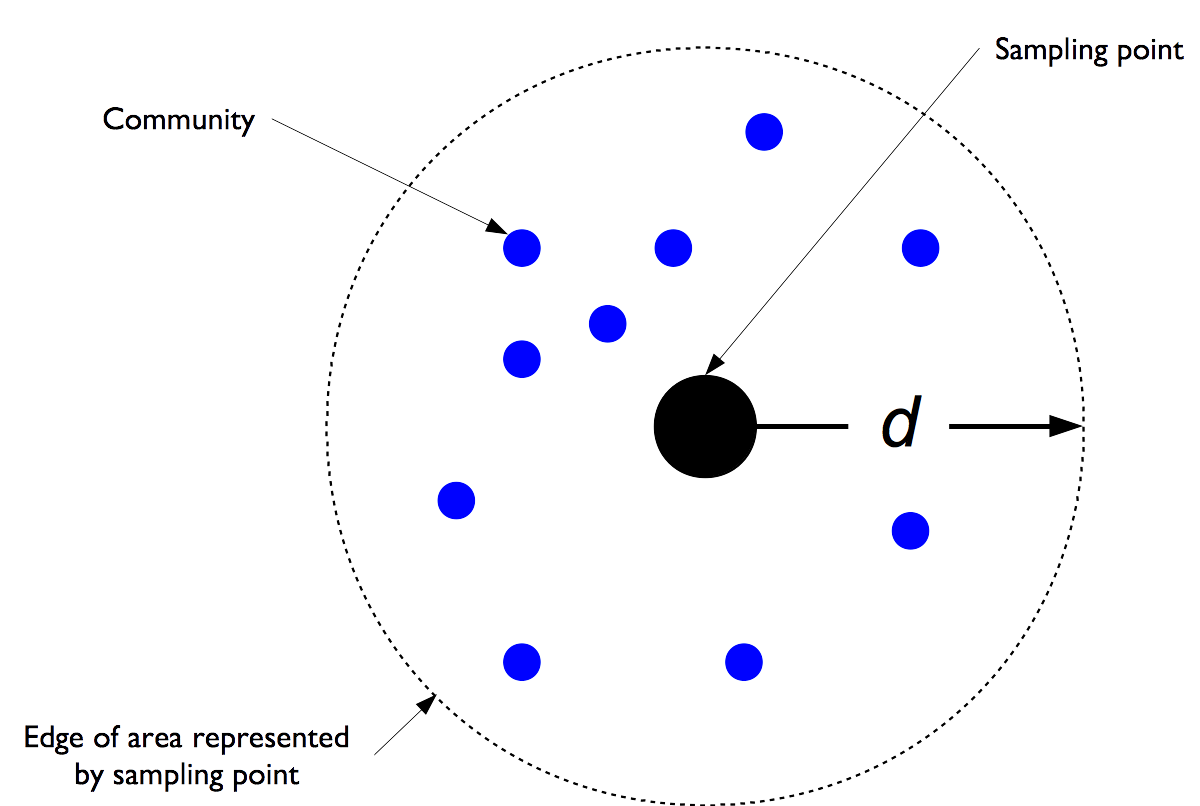
\includegraphics[width=16.67in]{figures/step2} 

}

\caption{Conceptual presentation of the area represented by each sampling point}\label{fig:distance1}
\end{figure}

~

There are other ways of thinking about \(d\). These are:

\begin{enumerate}
\def\labelenumi{\arabic{enumi}.}
\tightlist
\item
  \textbf{The area of each triangular tile}: This can be calculated
  using the formula:
\end{enumerate}

\[ A ~ = ~ \tan30^ \circ ~ \times ~ \frac{9}{4} ~ d ^ 2 \]

For \(d ~ = ~ 10 ~ \text{km}\) the area of each triangular tile will be
about:

\[ A ~ = ~ \tan30^ \circ ~ \times ~ \frac{9}{4} ~ d ^ 2 ~ \approx ~ 1.3 ~ \times ~ 100 ~ = ~ 130 ~ \text{km} ^ 2 \]

\begin{enumerate}
\def\labelenumi{\arabic{enumi}.}
\setcounter{enumi}{1}
\tightlist
\item
  \textbf{Practicability}: Most of the time spent in the field when
  doing a survey will be in travelling to and from sampling points.
  Having many sampling points can make for an expensive and / or lengthy
  survey. If you know how many sampling points that you can afford to
  take (\(m\)) then you can make a \textbf{very approximate} estimate of
  a suitable value for d using the following \emph{rule-of-thumb}
  formula:
\end{enumerate}

\[ d ~ \approx ~ \sqrt{\frac{\text{Program Area}}{m}} \]

The value of \(d\) calculated using this formula is approximate and
should be used as a starting point for a number of trial samples using
the procedure outlined below.

~

\begin{longtable}[]{@{}cccc@{}}
\toprule
\begin{minipage}[b]{0.14\columnwidth}\centering
\textbf{Pair}\strut
\end{minipage} & \begin{minipage}[b]{0.20\columnwidth}\centering
\textbf{Distance}\strut
\end{minipage} & \begin{minipage}[b]{0.14\columnwidth}\centering
\textbf{Pair}\strut
\end{minipage} & \begin{minipage}[b]{0.20\columnwidth}\centering
\textbf{Distance}\strut
\end{minipage}\tabularnewline
\midrule
\endhead
\begin{minipage}[t]{0.14\columnwidth}\centering
1\strut
\end{minipage} & \begin{minipage}[t]{0.20\columnwidth}\centering
21 km\strut
\end{minipage} & \begin{minipage}[t]{0.14\columnwidth}\centering
13\strut
\end{minipage} & \begin{minipage}[t]{0.20\columnwidth}\centering
13 km\strut
\end{minipage}\tabularnewline
\begin{minipage}[t]{0.14\columnwidth}\centering
2\strut
\end{minipage} & \begin{minipage}[t]{0.20\columnwidth}\centering
14 km\strut
\end{minipage} & \begin{minipage}[t]{0.14\columnwidth}\centering
14\strut
\end{minipage} & \begin{minipage}[t]{0.20\columnwidth}\centering
11 km\strut
\end{minipage}\tabularnewline
\begin{minipage}[t]{0.14\columnwidth}\centering
3\strut
\end{minipage} & \begin{minipage}[t]{0.20\columnwidth}\centering
13 km\strut
\end{minipage} & \begin{minipage}[t]{0.14\columnwidth}\centering
15\strut
\end{minipage} & \begin{minipage}[t]{0.20\columnwidth}\centering
12 km\strut
\end{minipage}\tabularnewline
\begin{minipage}[t]{0.14\columnwidth}\centering
4\strut
\end{minipage} & \begin{minipage}[t]{0.20\columnwidth}\centering
17 km\strut
\end{minipage} & \begin{minipage}[t]{0.14\columnwidth}\centering
16\strut
\end{minipage} & \begin{minipage}[t]{0.20\columnwidth}\centering
15 km\strut
\end{minipage}\tabularnewline
\begin{minipage}[t]{0.14\columnwidth}\centering
5\strut
\end{minipage} & \begin{minipage}[t]{0.20\columnwidth}\centering
11 km\strut
\end{minipage} & \begin{minipage}[t]{0.14\columnwidth}\centering
17\strut
\end{minipage} & \begin{minipage}[t]{0.20\columnwidth}\centering
13 km\strut
\end{minipage}\tabularnewline
\begin{minipage}[t]{0.14\columnwidth}\centering
6\strut
\end{minipage} & \begin{minipage}[t]{0.20\columnwidth}\centering
14 km\strut
\end{minipage} & \begin{minipage}[t]{0.14\columnwidth}\centering
18\strut
\end{minipage} & \begin{minipage}[t]{0.20\columnwidth}\centering
16 km\strut
\end{minipage}\tabularnewline
\begin{minipage}[t]{0.14\columnwidth}\centering
7\strut
\end{minipage} & \begin{minipage}[t]{0.20\columnwidth}\centering
12 km\strut
\end{minipage} & \begin{minipage}[t]{0.14\columnwidth}\centering
19\strut
\end{minipage} & \begin{minipage}[t]{0.20\columnwidth}\centering
18 km\strut
\end{minipage}\tabularnewline
\begin{minipage}[t]{0.14\columnwidth}\centering
8\strut
\end{minipage} & \begin{minipage}[t]{0.20\columnwidth}\centering
15 km\strut
\end{minipage} & \begin{minipage}[t]{0.14\columnwidth}\centering
20\strut
\end{minipage} & \begin{minipage}[t]{0.20\columnwidth}\centering
13 km\strut
\end{minipage}\tabularnewline
\begin{minipage}[t]{0.14\columnwidth}\centering
9\strut
\end{minipage} & \begin{minipage}[t]{0.20\columnwidth}\centering
16 km\strut
\end{minipage} & \begin{minipage}[t]{0.14\columnwidth}\centering
21\strut
\end{minipage} & \begin{minipage}[t]{0.20\columnwidth}\centering
8 km\strut
\end{minipage}\tabularnewline
\begin{minipage}[t]{0.14\columnwidth}\centering
10\strut
\end{minipage} & \begin{minipage}[t]{0.20\columnwidth}\centering
12 km\strut
\end{minipage} & \begin{minipage}[t]{0.14\columnwidth}\centering
22\strut
\end{minipage} & \begin{minipage}[t]{0.20\columnwidth}\centering
16 km\strut
\end{minipage}\tabularnewline
\begin{minipage}[t]{0.14\columnwidth}\centering
11\strut
\end{minipage} & \begin{minipage}[t]{0.20\columnwidth}\centering
17 km\strut
\end{minipage} & \begin{minipage}[t]{0.14\columnwidth}\centering
23\strut
\end{minipage} & \begin{minipage}[t]{0.20\columnwidth}\centering
18 km\strut
\end{minipage}\tabularnewline
\begin{minipage}[t]{0.14\columnwidth}\centering
12\strut
\end{minipage} & \begin{minipage}[t]{0.20\columnwidth}\centering
14 km\strut
\end{minipage} & \begin{minipage}[t]{0.14\columnwidth}\centering
24\strut
\end{minipage} & \begin{minipage}[t]{0.20\columnwidth}\centering
14 km\strut
\end{minipage}\tabularnewline
\bottomrule
\end{longtable}

~

\begin{figure}[H]

{\centering 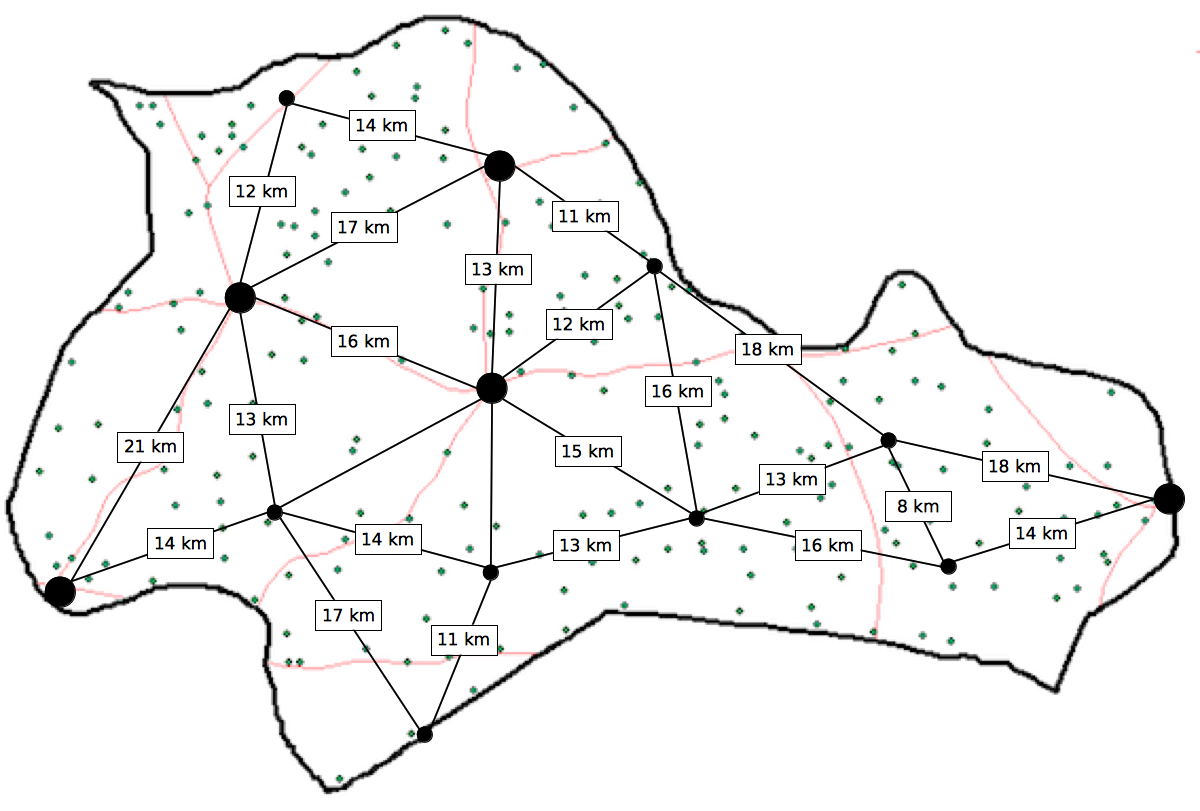
\includegraphics[width=16.67in]{figures/step2a} 

}

\caption{Distances of communities to the nearest substantial markets}\label{fig:distance2}
\end{figure}

~

\BeginKnitrBlock{rmdcalc}
Following are steps to estimate value of \(d\) based on distances that
carers are willing or able to walk to access services.

~

Using the information from the distance table, add the distances
together:

\[ \sum \text{Distance} ~ = ~ 343 ~ \text{km} \]

~

Divide the result by the number of paired distances:

\[ \frac{\sum \text{Distance}}{\text{Number of paired distances}} ~ = ~ \frac{343}{24} ~ = ~ 14.29 ~ \text{km} \]

~

Divide the result by two:

\[ d ~ = ~ \frac{14.29}{2} ~ = ~ 7.15 ~ \approx ~ 7 ~ \text{km} \]
\EndKnitrBlock{rmdcalc}

~

This is an estimate of the distance that carers are willing or able to
walk to access services. Only distances between towns and villages with
markets are used in this calculation.

A way of deciding a value for \(d\) that is based on the economic
geography of the survey area is to set \(d\) to one half of the mean
distance between neighbouring pairs of communities with substantial
markets.

S3M surveys have been done using a wide range (i.e.~from
\(d ~ = ~ 8 ~ \text{km}\) to \(d ~ = ~ 33 ~ \text{km}\)) of values for
\(d\). A value for \(d\) of 10 km or 12 km will probably be small enough
in most circumstances.

\newpage

\hypertarget{step-3-draw-a-grid-over-the-map}{%
\subsection{Step 3: Draw a grid over the
map}\label{step-3-draw-a-grid-over-the-map}}

\begin{figure}[H]

{\centering 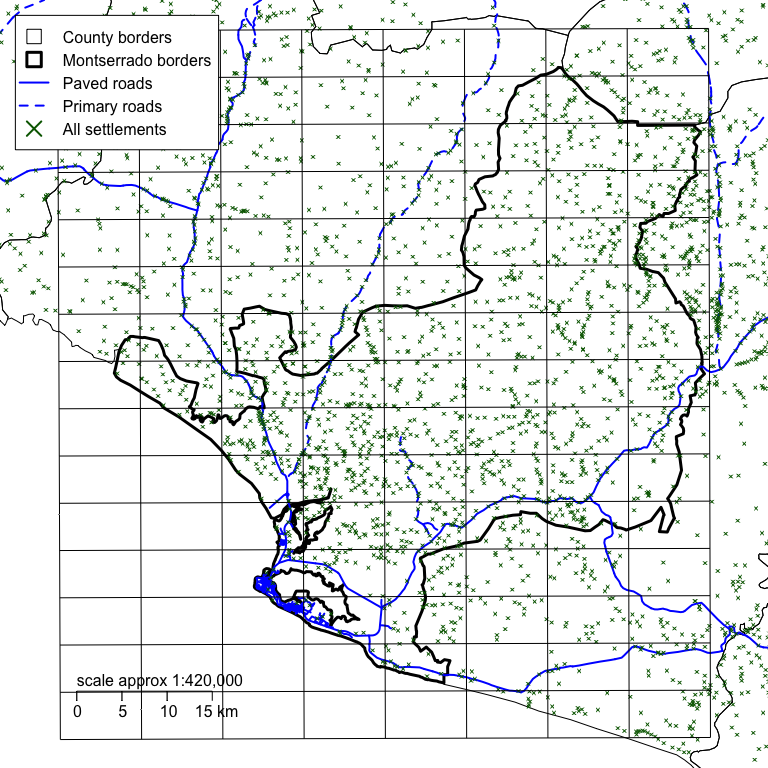
\includegraphics{figures/grid1-1} 

}

\caption{Montserrado county with a rectangular grid defined by d of 6 km}\label{fig:grid1}
\end{figure}

\newpage

\begin{figure}[H]

{\centering 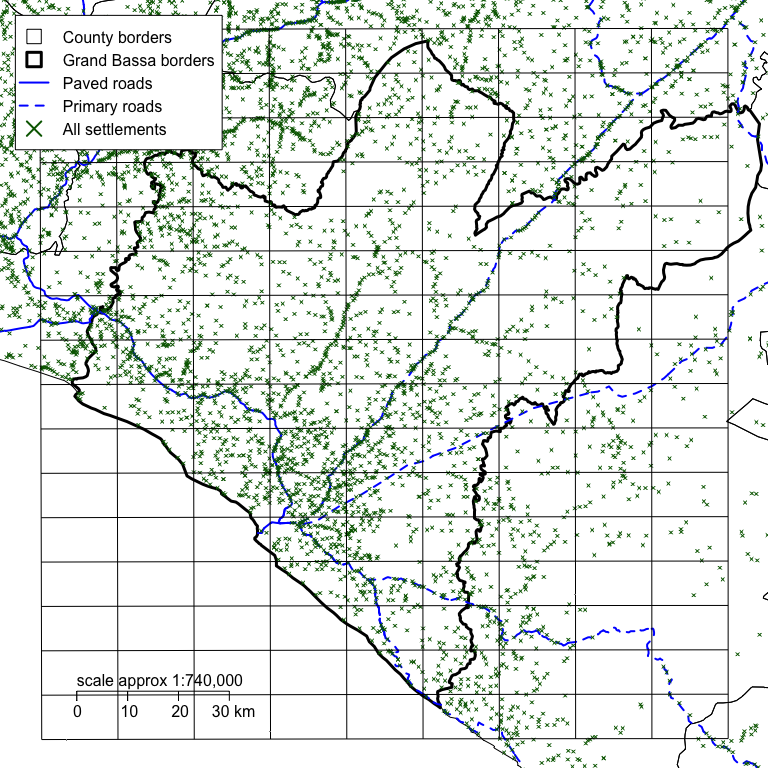
\includegraphics{figures/grid1a-1} 

}

\caption{Grand Bassa county with a rectangular grid defined by d of 10 km}\label{fig:grid1a}
\end{figure}

~

The next step is to draw a grid over the map.

The size of the grid is determined by the distance (\(d\)) that you
decided in \textbf{Step 2}.

The grid is rectangular rather than square. This allows us to place
sampling points at the centres of hexagons in a hexagonal grid without
the need to draw a hexagonal grid (see \textbf{Step 4}).

The width of the grid in the east-west (\(x\)) direction is different
from the height of the grid in the north-south (\(y\)) direction.

The width of the grid in the east-west (\(x\)) direction is calculated
using:

\[ x ~ = ~ \frac{3d}{2} \]

where \(d\) is the distance (\(d\)) that you decided in \textbf{Step 2}.

The height of the grid in the north-south (\(y\)) direction can be
calculated using:

\[ y ~ = ~ \frac{\sqrt{3}d}{2} \]

where \(d\) is the distance (\(d\)) that you decided in \textbf{Step 2}.

For example, in Figure \ref{fig:grid1}, we used
\(d ~ = ~ 6 ~ \text{km}\). This value of \(d\) creates a rectangular
grid with the following dimensions:

\[ x ~ = ~ \frac{3d}{2} ~ = ~ \frac{3 ~ \times ~ 6}{2} ~ = ~ \frac{18}{2} ~ = ~ 9 ~ \text{km} \]

and:

\[ y ~ = ~ \frac{\sqrt{3}d}{2} ~ \approx ~ \frac{1.73 ~ \times ~ 6}{2} ~ \approx ~ \frac{10.38}{2} ~ \approx ~ 5.2 ~ \text{km} \]

So, the grid in Figure \ref{fig:grid1} is 9 km long on the east-west
direction and 5.2 km on the north and south direction.

\newpage

The table below shows the grid sizes for different values of \(d\):

\begin{longtable}[]{@{}rrrlrrr@{}}
\toprule
\begin{minipage}[b]{0.10\columnwidth}\raggedleft
\textbf{d}\strut
\end{minipage} & \begin{minipage}[b]{0.14\columnwidth}\raggedleft
\textbf{x}\strut
\end{minipage} & \begin{minipage}[b]{0.14\columnwidth}\raggedleft
\textbf{y}\strut
\end{minipage} & \begin{minipage}[b]{0.06\columnwidth}\raggedright
\strut
\end{minipage} & \begin{minipage}[b]{0.10\columnwidth}\raggedleft
\textbf{d}\strut
\end{minipage} & \begin{minipage}[b]{0.14\columnwidth}\raggedleft
\textbf{x}\strut
\end{minipage} & \begin{minipage}[b]{0.14\columnwidth}\raggedleft
\textbf{y}\strut
\end{minipage}\tabularnewline
\midrule
\endhead
\begin{minipage}[t]{0.10\columnwidth}\raggedleft
5\strut
\end{minipage} & \begin{minipage}[t]{0.14\columnwidth}\raggedleft
7.5\strut
\end{minipage} & \begin{minipage}[t]{0.14\columnwidth}\raggedleft
4.3\strut
\end{minipage} & \begin{minipage}[t]{0.06\columnwidth}\raggedright
\strut
\end{minipage} & \begin{minipage}[t]{0.10\columnwidth}\raggedleft
13\strut
\end{minipage} & \begin{minipage}[t]{0.14\columnwidth}\raggedleft
19.5\strut
\end{minipage} & \begin{minipage}[t]{0.14\columnwidth}\raggedleft
11.3\strut
\end{minipage}\tabularnewline
\begin{minipage}[t]{0.10\columnwidth}\raggedleft
6\strut
\end{minipage} & \begin{minipage}[t]{0.14\columnwidth}\raggedleft
9.0\strut
\end{minipage} & \begin{minipage}[t]{0.14\columnwidth}\raggedleft
5.2\strut
\end{minipage} & \begin{minipage}[t]{0.06\columnwidth}\raggedright
\strut
\end{minipage} & \begin{minipage}[t]{0.10\columnwidth}\raggedleft
14\strut
\end{minipage} & \begin{minipage}[t]{0.14\columnwidth}\raggedleft
21.0\strut
\end{minipage} & \begin{minipage}[t]{0.14\columnwidth}\raggedleft
12.1\strut
\end{minipage}\tabularnewline
\begin{minipage}[t]{0.10\columnwidth}\raggedleft
7\strut
\end{minipage} & \begin{minipage}[t]{0.14\columnwidth}\raggedleft
10.5\strut
\end{minipage} & \begin{minipage}[t]{0.14\columnwidth}\raggedleft
6.1\strut
\end{minipage} & \begin{minipage}[t]{0.06\columnwidth}\raggedright
\strut
\end{minipage} & \begin{minipage}[t]{0.10\columnwidth}\raggedleft
15\strut
\end{minipage} & \begin{minipage}[t]{0.14\columnwidth}\raggedleft
22.5\strut
\end{minipage} & \begin{minipage}[t]{0.14\columnwidth}\raggedleft
13.0\strut
\end{minipage}\tabularnewline
\begin{minipage}[t]{0.10\columnwidth}\raggedleft
8\strut
\end{minipage} & \begin{minipage}[t]{0.14\columnwidth}\raggedleft
12.0\strut
\end{minipage} & \begin{minipage}[t]{0.14\columnwidth}\raggedleft
6.9\strut
\end{minipage} & \begin{minipage}[t]{0.06\columnwidth}\raggedright
\strut
\end{minipage} & \begin{minipage}[t]{0.10\columnwidth}\raggedleft
16\strut
\end{minipage} & \begin{minipage}[t]{0.14\columnwidth}\raggedleft
24.0\strut
\end{minipage} & \begin{minipage}[t]{0.14\columnwidth}\raggedleft
13.9\strut
\end{minipage}\tabularnewline
\begin{minipage}[t]{0.10\columnwidth}\raggedleft
9\strut
\end{minipage} & \begin{minipage}[t]{0.14\columnwidth}\raggedleft
13,5\strut
\end{minipage} & \begin{minipage}[t]{0.14\columnwidth}\raggedleft
7.8\strut
\end{minipage} & \begin{minipage}[t]{0.06\columnwidth}\raggedright
\strut
\end{minipage} & \begin{minipage}[t]{0.10\columnwidth}\raggedleft
17\strut
\end{minipage} & \begin{minipage}[t]{0.14\columnwidth}\raggedleft
25.5\strut
\end{minipage} & \begin{minipage}[t]{0.14\columnwidth}\raggedleft
14.7\strut
\end{minipage}\tabularnewline
\begin{minipage}[t]{0.10\columnwidth}\raggedleft
10\strut
\end{minipage} & \begin{minipage}[t]{0.14\columnwidth}\raggedleft
15.0\strut
\end{minipage} & \begin{minipage}[t]{0.14\columnwidth}\raggedleft
8.7\strut
\end{minipage} & \begin{minipage}[t]{0.06\columnwidth}\raggedright
\strut
\end{minipage} & \begin{minipage}[t]{0.10\columnwidth}\raggedleft
18\strut
\end{minipage} & \begin{minipage}[t]{0.14\columnwidth}\raggedleft
27.0\strut
\end{minipage} & \begin{minipage}[t]{0.14\columnwidth}\raggedleft
15.6\strut
\end{minipage}\tabularnewline
\begin{minipage}[t]{0.10\columnwidth}\raggedleft
11\strut
\end{minipage} & \begin{minipage}[t]{0.14\columnwidth}\raggedleft
16.5\strut
\end{minipage} & \begin{minipage}[t]{0.14\columnwidth}\raggedleft
19.5\strut
\end{minipage} & \begin{minipage}[t]{0.06\columnwidth}\raggedright
\strut
\end{minipage} & \begin{minipage}[t]{0.10\columnwidth}\raggedleft
19\strut
\end{minipage} & \begin{minipage}[t]{0.14\columnwidth}\raggedleft
28.5\strut
\end{minipage} & \begin{minipage}[t]{0.14\columnwidth}\raggedleft
16.5\strut
\end{minipage}\tabularnewline
\begin{minipage}[t]{0.10\columnwidth}\raggedleft
12\strut
\end{minipage} & \begin{minipage}[t]{0.14\columnwidth}\raggedleft
18.0\strut
\end{minipage} & \begin{minipage}[t]{0.14\columnwidth}\raggedleft
10.4\strut
\end{minipage} & \begin{minipage}[t]{0.06\columnwidth}\raggedright
\strut
\end{minipage} & \begin{minipage}[t]{0.10\columnwidth}\raggedleft
20\strut
\end{minipage} & \begin{minipage}[t]{0.14\columnwidth}\raggedleft
30.0\strut
\end{minipage} & \begin{minipage}[t]{0.14\columnwidth}\raggedleft
17.3\strut
\end{minipage}\tabularnewline
\bottomrule
\end{longtable}

When drawing the grid make sure that it covers the entire survey area.

It is usually best to draw a grid that covers an area that is a little
larger than the entire survey area. This helps to ensure that the survey
will sample from the entire survey area.

The grid can be drawn using marker pens onto plastic film overlaying the
map. This protects the map and allows you to reposition the grid to
improve the coverage of the sample should this be needed.

If you are drawing the grid directly onto the map then use a soft pencil
(e.g.~a \emph{2B} or \emph{\#1} pencil). A soft pencil will not damage
the surface of the map and is easy to erase using a soft rubber eraser
should you make a mistake or need to draw a different grid.

\newpage

\hypertarget{step-4-create-an-even-spread-of-sampling-points}{%
\subsection{Step 4: Create an even spread of sampling
points}\label{step-4-create-an-even-spread-of-sampling-points}}

\begin{figure}[H]

{\centering 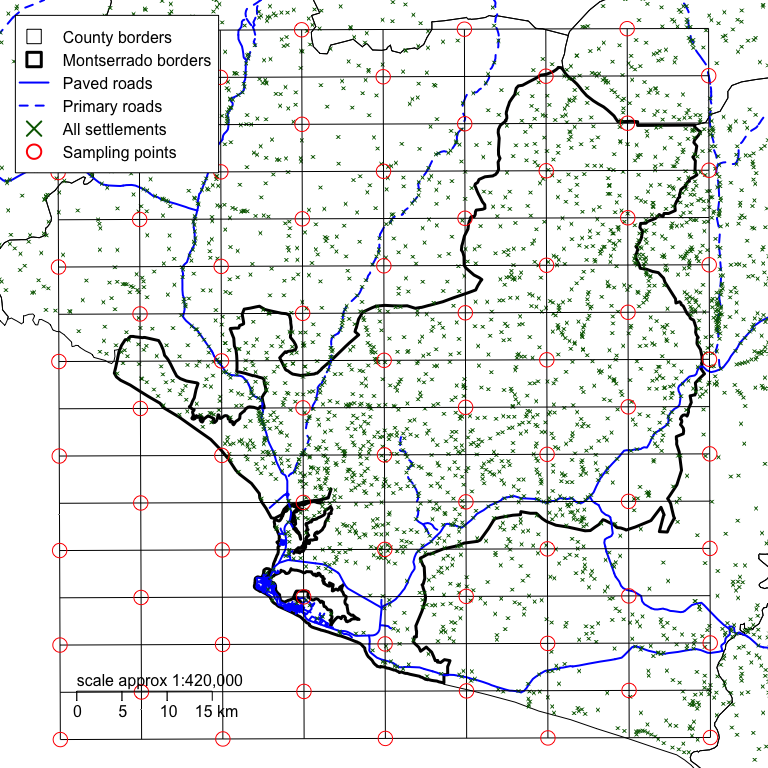
\includegraphics{figures/grid2-1} 

}

\caption{Montserrado county with a rectangular grid defined by d of 6 km and alternating intersections of the grid used to identify sampling points}\label{fig:grid2}
\end{figure}

\newpage

\begin{figure}[H]

{\centering 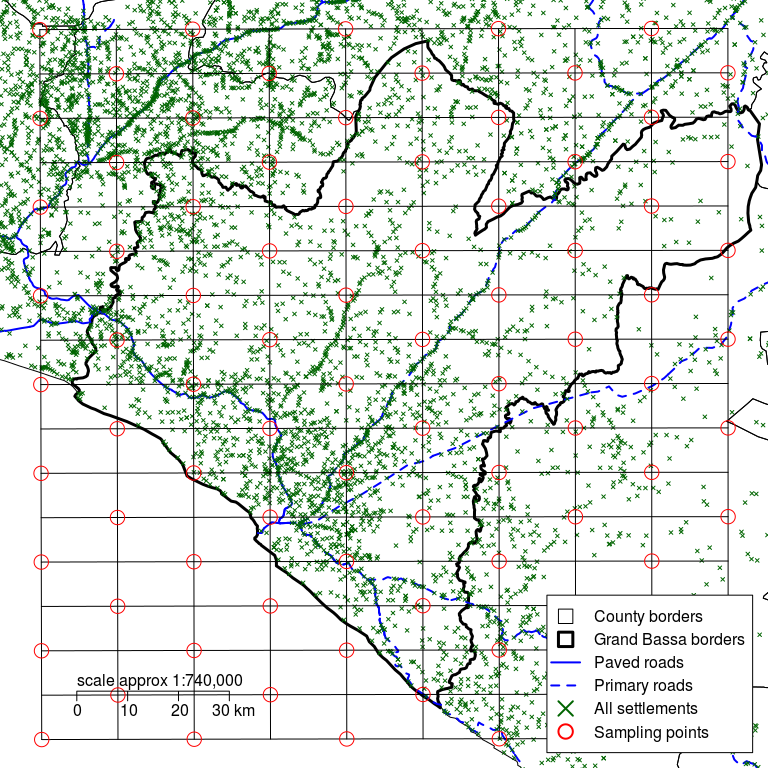
\includegraphics{figures/grid2a-1} 

}

\caption{Grand Bassa county with a rectangular grid defined by d of 10 km and alternating intersections of the grid used to identify sampling points}\label{fig:grid2a}
\end{figure}

Sampling points are located at the intersections of the rectangular grid
in a staggered fashion. Alternate intersections of the grid in the x
(east-west) and y (north-south) directions are used:

\newpage

\begin{figure}[H]

{\centering 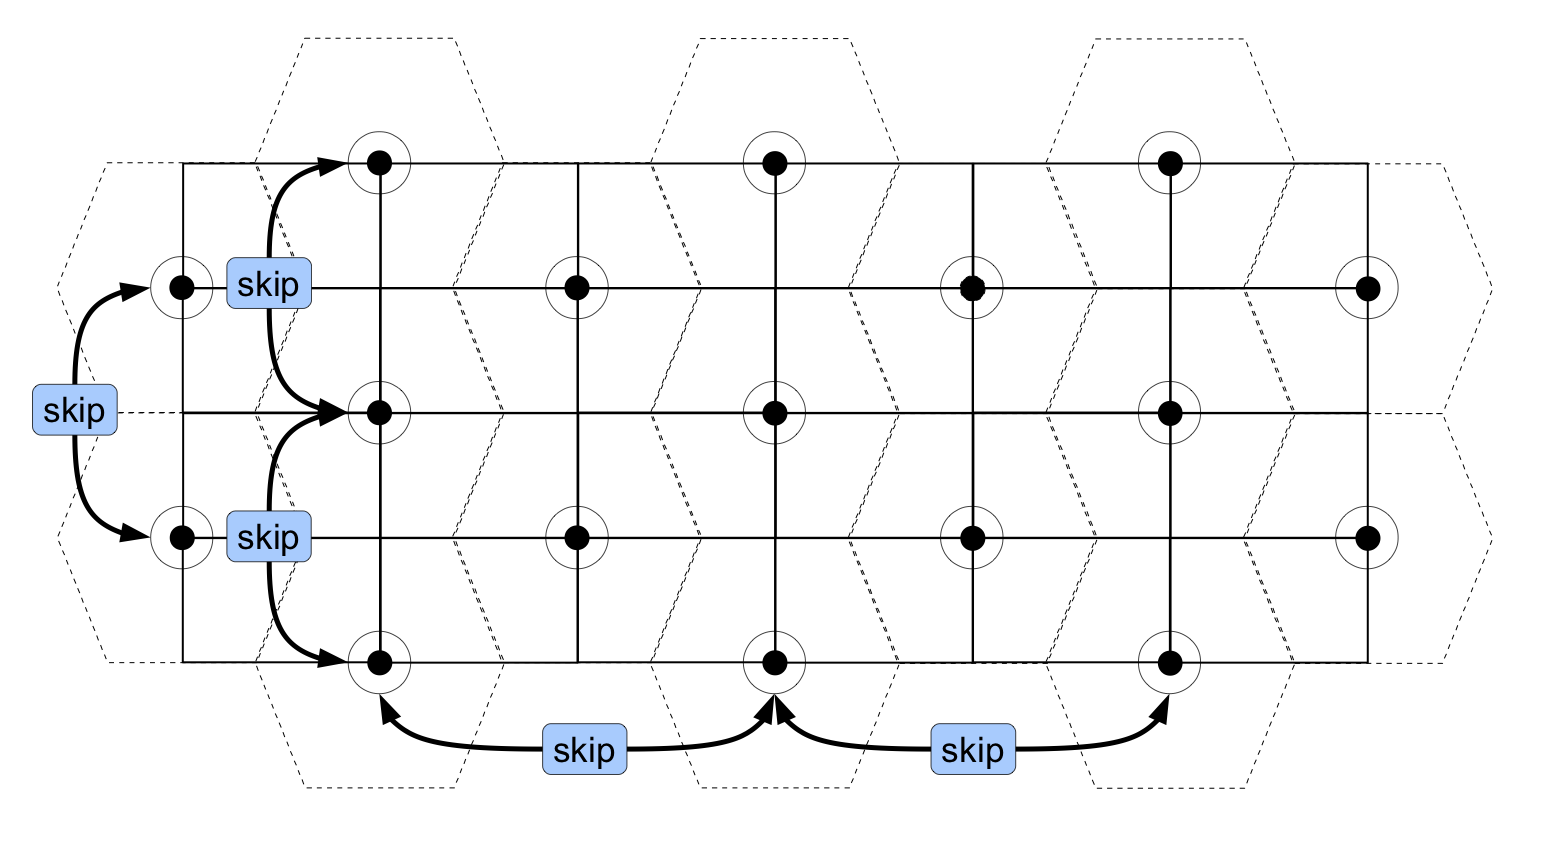
\includegraphics[width=21.46in]{figures/grid2a} 

}

\caption{Selecting alternating intersections of the grid in the x and y directions to spread sampling points evenly}\label{fig:grid2b}
\end{figure}

Note how this process places sampling points at the centres of hexagons
in a hexagonal grid without the need to draw a hexagonal grid.

Make sure that your sample points go right to the edge (or even over the
edge) of the survey area. This helps to ensure that the survey will
sample from the entire survey area.

\newpage

\hypertarget{step-5-select-the-communities-to-sample}{%
\subsection{Step 5: Select the communities to
sample}\label{step-5-select-the-communities-to-sample}}

\begin{figure}[H]

{\centering 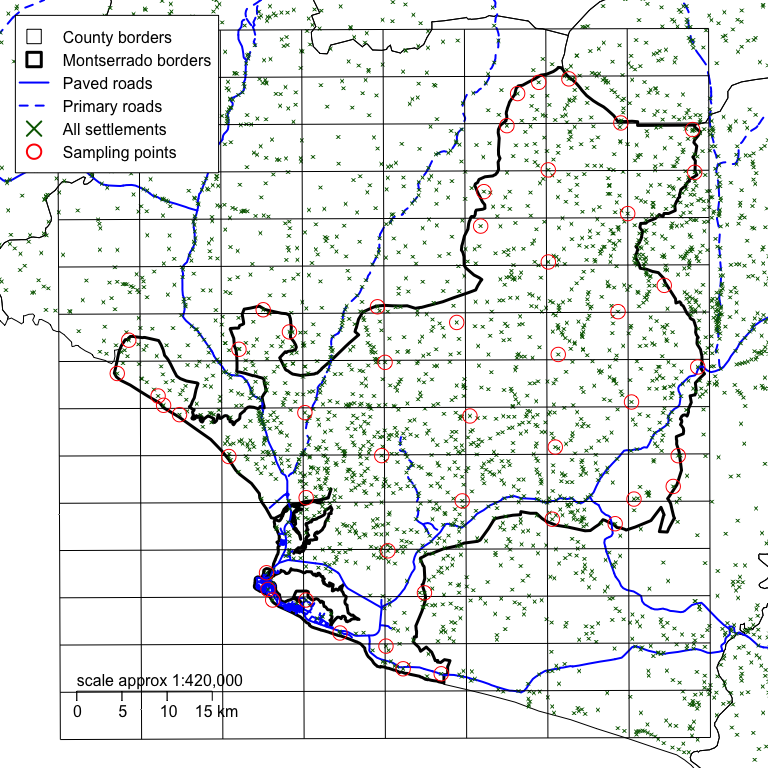
\includegraphics{figures/grid3-1} 

}

\caption{Montserrado county with a rectangular grid defined by d of 6 km and sampling points moved to the nearest communities}\label{fig:grid3}
\end{figure}

\newpage

\begin{figure}[H]

{\centering 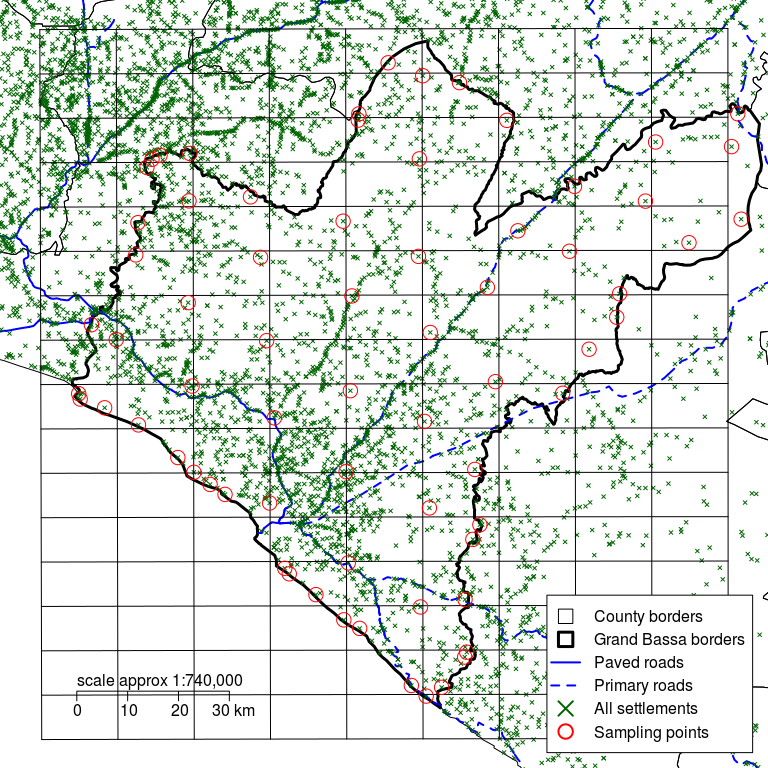
\includegraphics{figures/grid4-1} 

}

\caption{Grand Bassa county with a rectangular grid defined by d of 10 km and sampling points moved to the nearest communities}\label{fig:grid4}
\end{figure}

Select the community (or communities) closest to the sampling points
identified in \textbf{Step 4}.

The position of the sampling point is moved to the position of the
selected community. This is shown in the diagram above.

You may drop sampling points if you find that many sampling points are
clustered closely together.

You may move or add sampling points if you find that there are populated
areas that do not contain sampling points.

The aim is to create a roughly even spread of sampling points over the
entire survey area.

\BeginKnitrBlock{rmdcaution}
The S3M sample is defined using a systematic sampling method. Like any
systematic sampling method, an S3M sample can produce biased estimates
if there is periodic variation in prevalence and / or coverage and the
sampling points tend to coincide with this periodicity. This is
difficult to control for without prior knowledge of the periodic
variation, although simple checks such as ensuring that sampling points
are not all in valleys or all on hilltops, and adjusting the grid
position accordingly, should help to minimise this problem.
\EndKnitrBlock{rmdcaution}

\begin{figure}[H]

{\centering 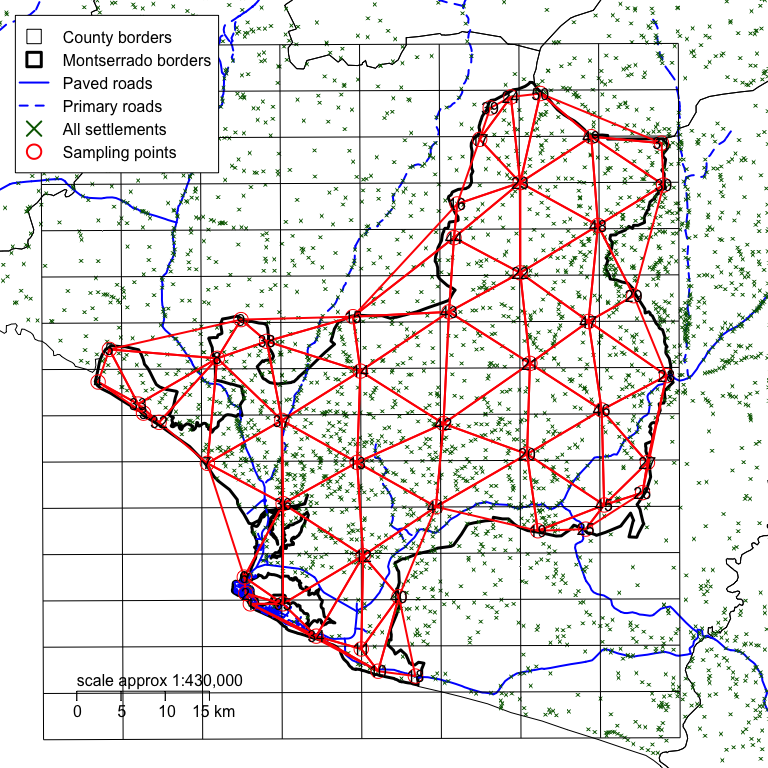
\includegraphics{figures/grid3a-1} 

}

\caption{Montserrado county with a rectangular grid defined by d of 6 km and sampling points moved to the nearest communities showing test triangulation}\label{fig:grid3a}
\end{figure}

\begin{figure}[H]

{\centering 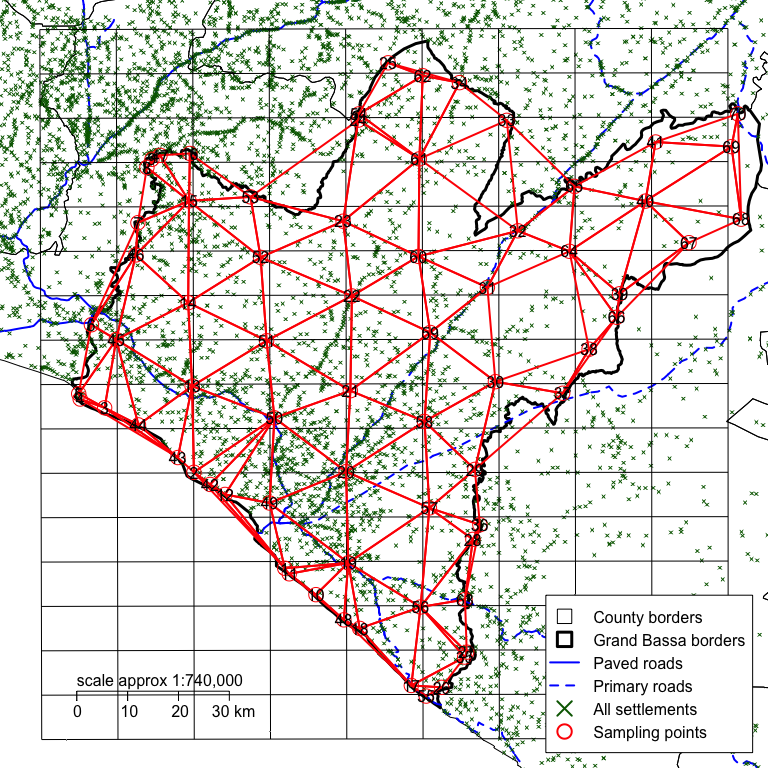
\includegraphics{figures/grid4a-1} 

}

\caption{Grand Bassa county with a rectangular grid defined by d of 10 km and sampling points moved to the nearest communities showing test triangulation}\label{fig:grid4a}
\end{figure}

A good way to check if you have an even spread of sampling points over
the entire survey area is to do a trial \emph{triangulation} of the
selected sampling points. This involves dividing up the survey area into
non-overlapping triangles with a sampling point at each vertex.

There will usually be many ways to divide the survey area into
triangles. The best triangulation is one that results in small
equilateral triangles (i.e.~triangles with all sides of equal length) or
small and nearly equilateral triangles. Avoid long and narrow triangles.
Avoid large triangles.

\begin{figure}[H]

{\centering 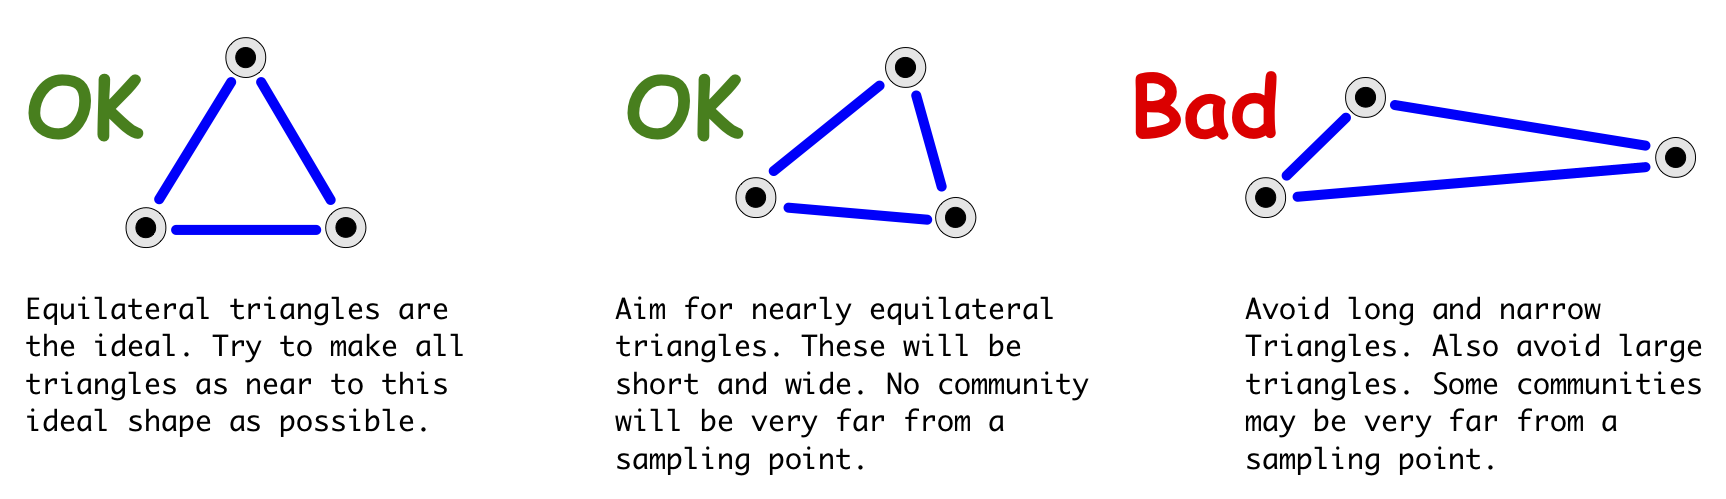
\includegraphics[width=23.97in]{figures/grid3a} 

}

\caption{Selecting alternating intersections of the grid in the x and y directions to spread sampling points evenly}\label{fig:grid3b}
\end{figure}

You can triangulate ``by eye'' or automatically (i.e.~using a computer).
If you use a computer to do this then you should use software that
produces a \emph{Delaunay triangulation}.

You may drop sampling points if you find that many sampling points are
clustered closely together.

You may move or add sampling points if you find that there are populated
areas that do not contain sampling points.

The aim is to create a roughly even spread of sampling points over the
entire survey area.

\newpage

\begin{figure}[H]

{\centering 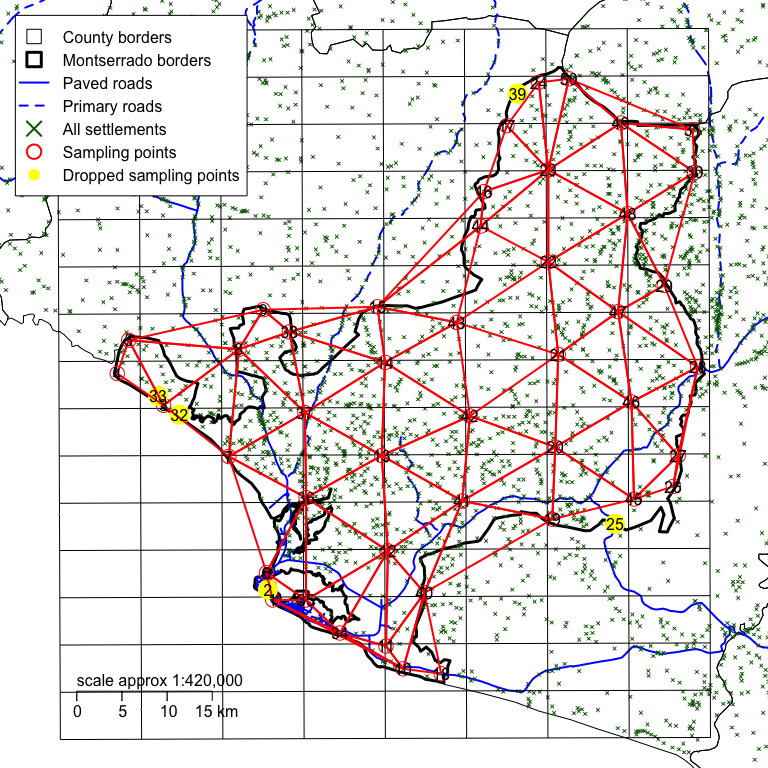
\includegraphics{figures/grid3c-1} 

}

\caption{Montserrado county with a rectangular grid defined by d of 6 km and sampling points moved to the nearest communities showing updated triangulation}\label{fig:grid3c}
\end{figure}

\begin{figure}[H]

{\centering 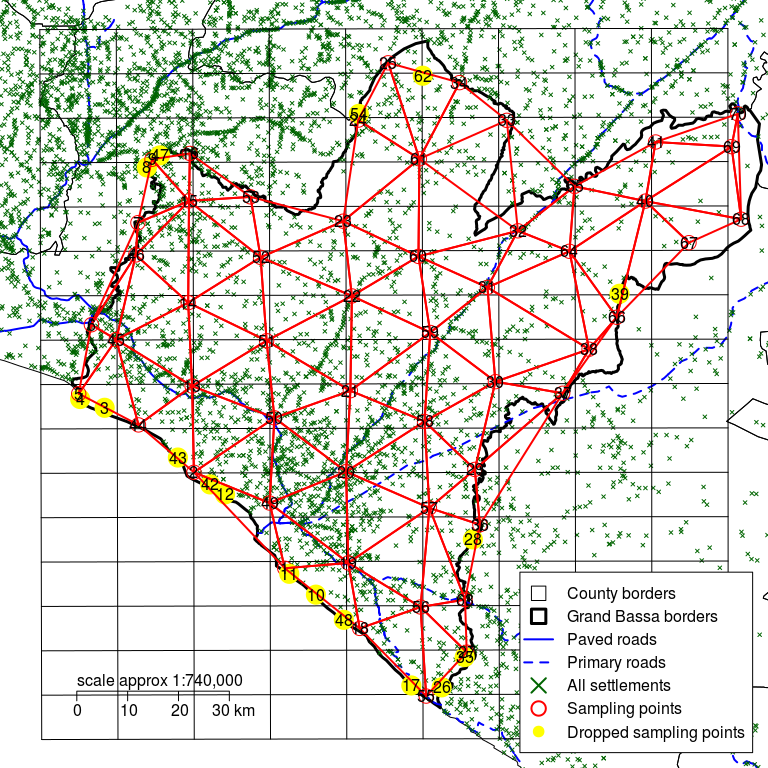
\includegraphics{figures/grid4c-1} 

}

\caption{Grand Bassa county with a rectangular grid defined by d of 10 km and sampling points moved to the nearest communities showing updated triangulation}\label{fig:grid4c}
\end{figure}

Figure \ref{fig:grid3c} above show a trial triangulation for Montserrado
county with only a few long and narrow triangles. Five sampling points
(labelled 2, 25, 32, 33, 39) have been dropped to ensure that there are
few long and narrow triangles.

Figure \ref{fig:grid4c} above show a trial triangulation for Grand Bassa
county with only a few long and narrow triangles. Seventeen sampling
points (labelled 3, 4, 8, 10, 11, 12, 17, 26, 28, 35, 39, 42, 43, 47,
48, 54, 62) have been dropped to ensure that there are a few long and
narrow triangles.

\newpage

\textbf{The sample will, to some extent, be dictated by the distribution
of communities in the survey area. It is usual to find that you have
some large triangles and some long and narrow triangles in your final
triangulation. You should try to keep the number of these ``problem''
triangles to a minimum.}

The process of selecting communities to sample is:

\begin{enumerate}
\def\labelenumi{\arabic{enumi}.}
\item
  Start by defining the sample using the grid based approach outlined
  above.
\item
  Use a trial triangulation. This can be done ``by eye'' or using a
  computer. Check for an even spatial sample:
\end{enumerate}

\begin{itemize}
\item
  Most triangles should be short and wide.
\item
  Very few triangles should be long and narrow.
\item
  The triangles should be of roughly equal size.
\item
  The complete set of triangles should cover all (or almost all) of the
  survey area.
\end{itemize}

\begin{enumerate}
\def\labelenumi{\arabic{enumi}.}
\setcounter{enumi}{2}
\tightlist
\item
  Move or add sampling points to improve the sample (i.e.~to avoid long
  and narrow triangles, to avoid large triangles, to make triangles
  roughly equal in size, and to ensure the sample covers all or almost
  all of the survey area). Triangulate again. Repeat this process until
  you are happy with the sample.
\end{enumerate}

\hypertarget{stage2}{%
\section{The second stage sample}\label{stage2}}

The second stage sample is also called \emph{within-community sampling}.
The sampling process that you use to select a sample from a community
will depend on what the survey is investigating.

If you are investigating multiple indicators which apply to different
groups of individuals then you may find it easier to use different
sampling methods for different indicators. You can think of this as
having different surveys for different indicators sampled from the same
set of communities at the same time. For the Liberia S3M, this is the
approach that will be used in which there will be 2 concurrent surveys.
There will be a survey for CMAM coverage which will be specific for SAM
children and a survey for children aged 6 - 59 months and their mothers.

\hypertarget{stage-2-sampling-for-cmam-coverage-survey}{%
\subsection{Stage 2 sampling for CMAM coverage
survey}\label{stage-2-sampling-for-cmam-coverage-survey}}

For the survey for CMAM coverage, an active and adaptive (snowball)
case-finding method can be used in stage 2 sampling to find all or
nearly all SAM cases by MUAC in the stage 1 sample \citep{Myatt:2012tt}.
However, given that the Liberia CMAM programme uses both MUAC and
weight-for-height as independent criteria for SAM, it is uncertain
whether the use of active and adaptive case finding using
weight-for-height will find all or nearly all SAM cases by
weight-for-height\footnote{Capture and re-capture studies done to test
  the sensitivity of active and adaptive case-finding as a sampling
  approach to find all or nearly all SAM cases were all implemented
  using MUAC as the indicator for SAM (see \citet{Wegerdt:2006ux}).}. It
is therefore recommended that a full census of children aged 6-59 months
in the selected villages in the stage 1 sample be conducted to ensure
exhaustivity. This will also be the approach to use in urban areas given
that active and adaptive case finding has been known to fail in finding
all SAM cases when implemented in urban areas \citep{Myatt:2012tt}. As
an example, the only other known coverage survey conducted in Liberia is
that which was conducted by Accion contra la faim in 2011 to assess
coverage of CMAM in Greater Monrovia \citep{AccionContralaFaim:2011vu}.
In this survey, it was unclear as to whether both MUAC and
weight-for-height was used to identify SAM but both active adaptive case
finding and mass screening was used to ensure that all or nearly all CAM
cases are found. Doing both approaches will be too resource-intensive. A
good census sample taken house-to-house or door-to-door should be
sufficient.

\hypertarget{stage-2-sampling-for-children-6-59-months-and-their-mothers}{%
\subsection{Stage 2 sampling for children 6-59 months and their
mothers}\label{stage-2-sampling-for-children-6-59-months-and-their-mothers}}

Given that the stage 2 sample for the CMAM coverage survey will utilise
a house-to-house or door-to-door of the villages, the stage 2 sample for
the survey of children 6-59 months old and their mothers can be done via
door/house counting with systematic selection in the first village
selected per sampling point.

Generally, in rural villages/communities, the village leader will know
how many houses/households are in the village so they can be asked for
this information. In urban locations/communities/blocks, this
information isn't usually known. So, door counting of the urban location
or block will be necessary to know the total number of doors/houses in
that particular urban area/location.

Once the number of houses or number of doors has been established, a
sampling interval will need to be calculated as follows:

~

\[ n_{\text{Sampling interval}} ~ = ~ \frac{\text{Total number of houses/doors}}{\text{Target sample of children 6-59 months old in village}} \]

~

The house-to-house/door-to-door sampling to look for SAM children can
start and then for every \(nth\) house/door, the survey for children
6-59 months old will be conducted as well.

Remember that this will be done in the first village selected per
sampling point.

\hypertarget{special-considerations-for-large-villages}{%
\subsection{Special considerations for large
villages}\label{special-considerations-for-large-villages}}

If a sampling point is located in a large village or town then the
village or town can be divided into a set of segments and the entire
population of only a sample of these segments are then fully enumerated
for the SAM coverage survey. If this village is the first village of the
sampling point, then the door/house counting with systematic selection
will be applied only in the sample of segments selected.

\textbf{Segmentation} involves dividing a community into several parts
and taking part of the within-community sample from each
\textbf{segment}. With simple communities, segmentation is not required
and we take a single sample from the entire community using the
appropriate sampling method.

\hypertarget{segmentation}{%
\subsubsection{Segmentation}\label{segmentation}}

For more complicated communities we divide the community into several
parts or segments, such as a community made up of several clusters:

\begin{figure}[H]

{\centering 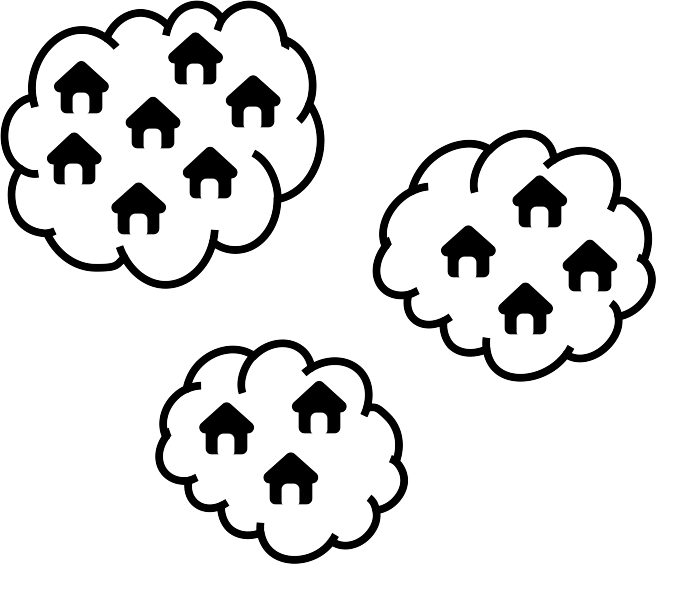
\includegraphics[width=9.72in]{figures/stage2sample3} 

}

\caption{Example of a set of clusters of dwellings}\label{fig:sample17}
\end{figure}

or a community made up of several ribbons:

\begin{figure}[H]

{\centering 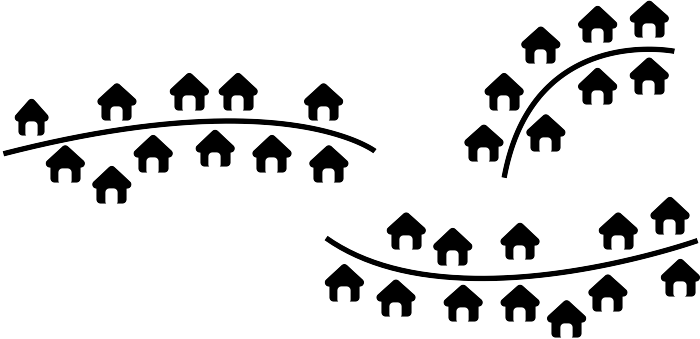
\includegraphics[width=9.72in]{figures/stage2sample4} 

}

\caption{Dwellings arranged in several lines}\label{fig:sample18}
\end{figure}

or a mixed community:

\begin{figure}[H]

{\centering 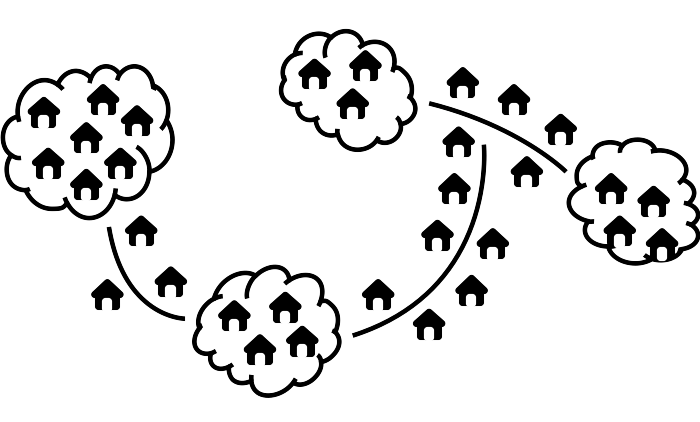
\includegraphics[width=9.72in]{figures/stage2sample5} 

}

\caption{Mixture of clusters and ribbons}\label{fig:sample19}
\end{figure}

Segments should be either ribbons or clusters but should \textbf{never}
contain both a ribbon and a cluster. This is because clusters and
ribbons are sampled in different ways.

To select which segments to sample in a very large village or in urban
locations/blocks, draw a rough map of the village and number each
segment. Then depending on how many segments have been decided to sample
(or are able to be sampled), select randomly the numbered segments. The
selected segments are then sampled house-to-house/door-to-door. If this
village is the first village of the sampling point, then the door/house
counting with systematic selection will be applied only in these
selected segments.

\hypertarget{samplesize}{%
\section{Sample size considerations}\label{samplesize}}

In general, the sample size needed for proportion-type indicators such
as those to be reported for this survey can be calculated using the
following equation.

\[\begin{aligned}
n & ~ = ~ Z^2 ~ \times ~ \frac{p(1 ~ - ~ p)}{c ^ 2} \\
\\
where: & \\
\\
Z & ~ = ~ \text{z-value for preferred confidence interval} \\
p & ~ = ~ \text{expected indicator proportion/prevalence} \\
c & ~ = ~ \text{level of precision}
\end{aligned}\]

The \(Z\) value is usually 1.96 for a 95\% confidence interval. The
\(p\) should usually be based on previous coverage results if available.
If not, it is usually appropriate to set \(p\) at 50\% (0.5) as this
results in the highest sample size estimate. The precision (\(c\)) for
coverage surveys is usually set at ±10\% based on standard precision
used for immunisation coverage.

Using these values, the typical sample size needed for coverage surveys
is about 96.

\[ n ~ = ~ 1.96^2 ~ \times ~ \frac{0.5(1 ~ - ~ 0.5)}{0.10 ^ 2} ~ \approx ~  96 \]

However, the survey design needs to be taken into account. A cluster
survey such as the one that is proposed for the Liberia S3M will need to
inflate sample sizes to account for the loss of variance due to the
cluster design. This inflation factor is called the \emph{design effect}
(\emph{DEFF}) which is based on the \emph{intracluster correlation
coefficient} (\emph{ICC}).

Generally, a \emph{DEFF} of 2 is used to multiply the sample size with
to account for the loss of variance. This would mean that a sample size
of 192 would be the target sample size.

The sample size required will also depend on the indicators being
assessed. Following is a further discussion of sample size requirements
for the CMAM coverage survey and for the survey for children 6-59 months
and their mothers.

\hypertarget{sample-size-for-the-cmam-coverage-survey}{%
\subsection{Sample size for the CMAM coverage
survey}\label{sample-size-for-the-cmam-coverage-survey}}

SAM treatment coverage can be demonstrated in the following equation:

\[ \text{SAM treatment coverage} ~ = ~ \frac{\text{SAM cases in treatment}}{\text{Total SAM cases}} \]

This indicator requires a sample of under 5 children who have SAM. SAM
children are rare (at most 3\% of the general population of children
under 5). This means that the universe population of SAM children is
small hence a finite population correction can be applied to sample size
calculations. At the same time, given the active adaptive case finding
approach that will be applied to finding SAM cases is know to be
exhaustive, \emph{DEFF} would generally be close to 1. Therefore, a
sample size of about 96 is generally big enough to estimate SAM
treatment coverage with a ±10\% precision.

\hypertarget{survey-for-children-aged-6-59-months-and-their-mothers}{%
\subsection{Survey for children aged 6-59 months and their
mothers}\label{survey-for-children-aged-6-59-months-and-their-mothers}}

For vitamin A supplementation, micronutrient powder supplementation,
IYCF counselling and ferrous sulphate-folic acid supplementation the
sample size of 192 would be the target sample size for each of these
indicators.

However, given that this is a compound sample such that the MNP
supplementation indicator is only for children 6-23 months old, the 192
sample will need to be inflated for the sample of children 6-59 months
old big enough to ensure that at least 192 children aged 6-23 months
will be included in the sample. The factor by which to inflate the
sample size for children 6-59 months old can be estimated as follows:

~

\[ \frac{\text{Age range in months for 6-59 month old children}}{\text{Age range in months for 6-23 month old children}} ~ = ~ \frac{59 - 6}{23 - 6} ~ = ~ \frac{53}{7} ~ \approx ~ 3 \]

~

The sample size for children aged 6-59 months old will need to be
inflated 3 times to ensure that a minimum sample size of 192 children
aged 6-23 months will be sampled.

So, our sample size for the survey for children 6-59 months old and
their mothers will be 576.

\hypertarget{urbanrural}{%
\section{Urban and rural sample considerations}\label{urbanrural}}

Currently, the requirements for the survey is to provide coverage
estimates for Montserrado rural districts and the whole Grand Bassa
county. Urban areas have been specifically excluded.

Given that urban areas would most likely have different characteristics
than rural areas, it is more reasonable to treat urban areas as a
separate survey area. If urban areas are to be sampled, then urban areas
should have its own sample with the same minimum sample size as
described above. The implication of this would be an extra survey for
each and every urban area to be assessed.

\hypertarget{samplingframe}{%
\section{Overall sampling frame}\label{samplingframe}}

Given the stage 1 sampling, stage 2 sampling and sample size
considerations described above, following are the overall sampling
frames for each of two surveys that will be conducted.

\hypertarget{sampling-frame-for-the-cmam-coverage-survey}{%
\subsection{Sampling frame for the CMAM coverage
survey}\label{sampling-frame-for-the-cmam-coverage-survey}}

Using an S3M approach to stage 1 sampling, thirty (30) stage 1 sampling
points will be identified. This is an adaptation of S3M such that
instead of first specifying a \(d\) value, a minimum number of stage 1
samples is specified based on which the hexagonal grid across each
county will be drawn. This would mean that each county will be divided
into 30 hexagonal, non-overlapping grids to identify 30 sampling points
as the stage 1 sample. If estimates for urban areas will be required,
then the urban areas of each county will be separated and a separate
grid of 30 hexagons will be drawn on the map of the urban areas.

UNICEF has selected Greater Monrovia District and Grand Bassa County as
the areas for the Liberia survey.

The Liberia Institute of Statistics and Geo-Informatic Services (LISGIS)
has provided PDF maps of Greater Monrovia District and Grand Bassa
County shown below.

~

\begin{figure}[H]

{\centering 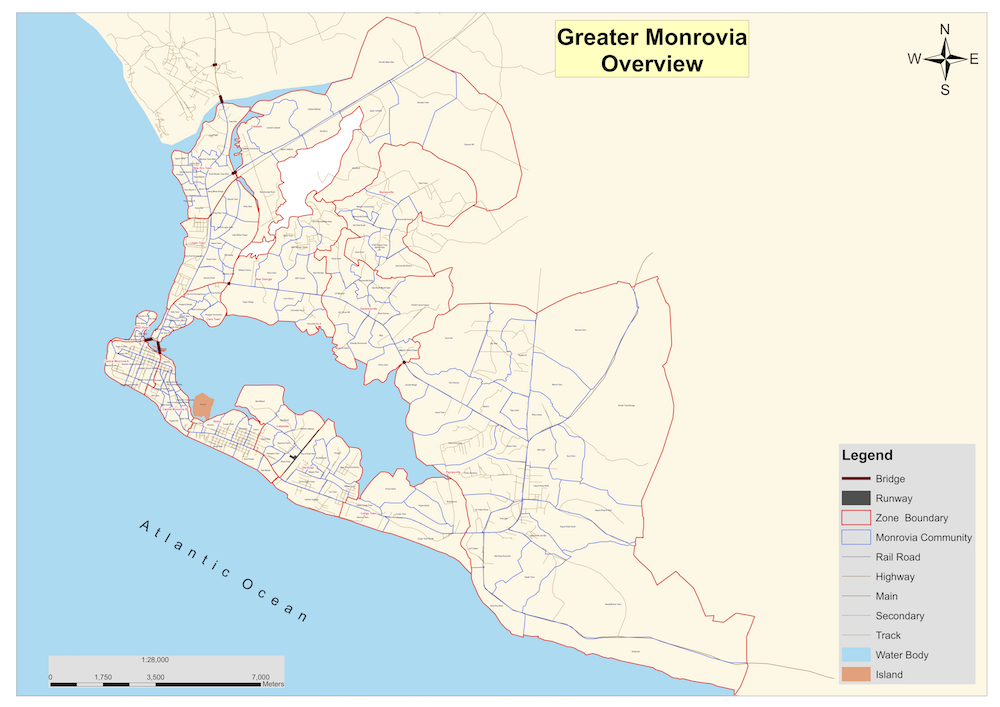
\includegraphics[width=0.8\linewidth]{figures/greaterMonroviaEA} 

}

\caption{Map of Greater Monrovia}\label{fig:sample20}
\end{figure}

~

\begin{figure}[H]

{\centering 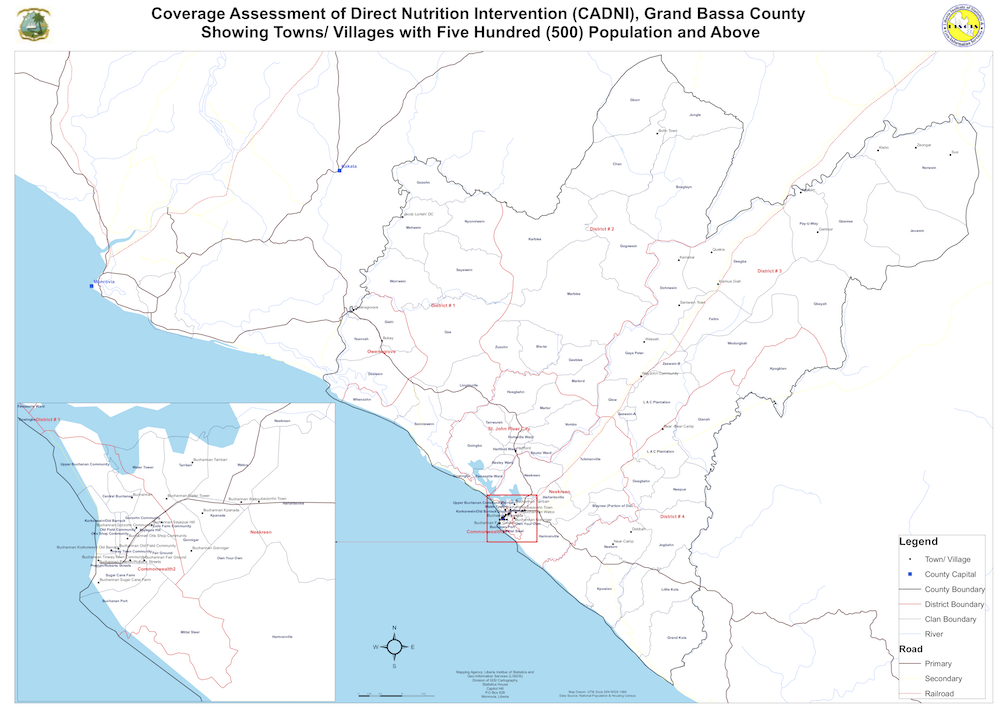
\includegraphics[width=0.8\linewidth]{figures/grandBassaEA} 

}

\caption{Map of Grand Bassa}\label{fig:sample21}
\end{figure}

~

Thirty hexagonal grids are then laid on top of these maps.

~

\begin{figure}[H]

{\centering 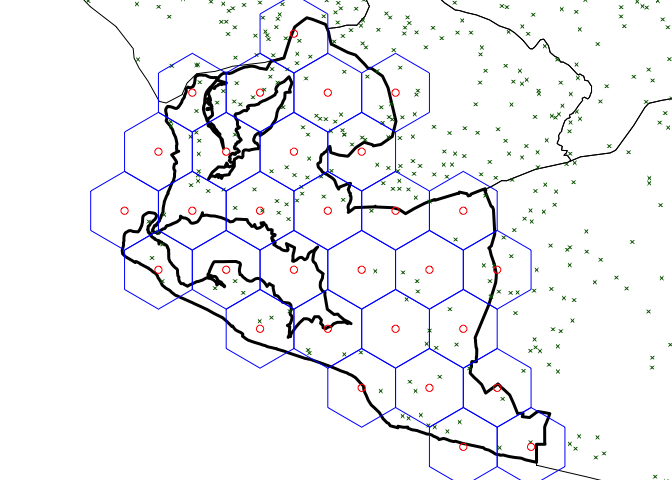
\includegraphics{figures/sample22-1} 

}

\caption{Thirty hexagonal grids laid on the  map of Greater Monrovia District}\label{fig:sample22}
\end{figure}

~

\begin{figure}[H]

{\centering 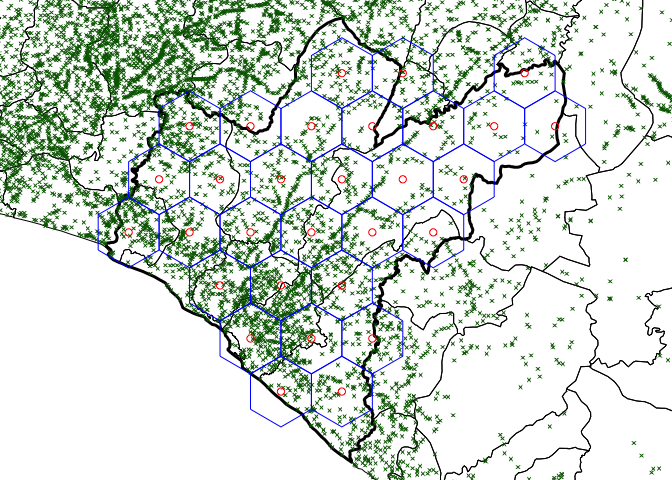
\includegraphics{figures/sample23-1} 

}

\caption{Thirty hexagonal grids laid on the  map of Grand Bassa County}\label{fig:sample23}
\end{figure}

~

To determine how many villages near the 30 sampling points to select for
the stage 1 sample, it would require estimating how many
villages/localities/communities/enumeration areas will need to be
sampled to obtain the target sample size of 96 SAM children in each
county and urban areas. This can be estimated as follows:

~

\[ n_{villages} ~ = ~ \frac{\text{Target sample size}}{n_{\text{average village population all ages}} ~ \times ~ \% ~ \text{under 5 children} ~ \times ~ \text{SAM prevalence}} \]

~

The average village population can be estimated using per
village/locality/community/enumeration area population in Grand Bassa
county and Greater Monrovia provided by the Liberia Institute of
Statistics and Geo-information Services to UNICEF.

For Greater Monrovia, the average enumeration area population is 5200.
For Grand Bassa (including urban areas) is 521 population per
enumeration area and 100 population per locality/village/community.

The proportion of children under 5 can be estimated using data from the
\href{https://www.census.gov/data-tools/demo/idb/region.php?N=\%20Results\%20\&T=15\&A=separate\&RT=0\&Y=2018\&R=-1\&C=LI}{US
Census Bureau} on estimated population for single years. Using this
data, the estimated proportion of under five children is about 17\%.

The SAM prevalence can be estimated as 3\% (based on communication with
UNICEF). This is most likely a high estimate considering that this is
the estimate for the whole country and not specific to the counties.
Also, seasonality of SAM prevalence will need to be taken into account.
If the period in which the survey is to be conducted is a season for low
prevalence of SAM, this should be considered in the estimation. So, it
might be good to use a lower estimate for SAM to ensure there is enough
villages sampled to get the target. An estimate of 1.5\% (or even lower)
is recommended.

Using these values, the number of villages needed to sample in each
county (and urban areas if included) can be calculated for each county
as follows:

~

\[\begin{aligned} 
n_{\text{Grand Bassa EA}} & ~ = ~ \left \lceil \frac{\text{Target sample size}}{n_{\text{average EA population all ages}} ~ \times ~ \% ~ \text{under 5 children} ~ \times ~ \text{SAM prevalence}} \right \rceil \\
\\
& ~ = ~ \left \lceil \frac{96}{521 ~ \times ~ 0.17 ~ \times ~ 0.015} \right \rceil \\
\\
& ~ = ~ \left \lceil \frac{96}{1.32855} \right \rceil \\
\\
& ~ \approx ~ 73
\end{aligned}\]

~

\[\begin{aligned} 
n_{\text{Grand Bassa villages}} & ~ = ~ \left \lceil \frac{\text{Target sample size}}{n_{\text{average village population all ages}} ~ \times ~ \% ~ \text{under 5 children} ~ \times ~ \text{SAM prevalence}} \right \rceil \\
\\
& ~ = ~ \left \lceil \frac{96}{100 ~ \times ~ 0.17 ~ \times ~ 0.015} \right \rceil \\
\\
& ~ = ~ \left \lceil \frac{96}{0.255} \right \rceil \\
\\
& ~ \approx ~ 377
\end{aligned}\]

\newpage

\[\begin{aligned} 
n_{\text{Greater Monrovia District EA}} & ~ = ~ \left \lceil \frac{\text{Target sample size}}{n_{\text{average EA population all ages}} ~ \times ~ \% ~ \text{under 5 children} ~ \times ~ \text{SAM prevalence}} \right \rceil \\
\\
& ~ = ~ \left \lceil \frac{96}{500 ~ \times ~ 0.17 ~ \times ~ 0.015} \right \rceil \\
\\
& ~ = ~ \left \lceil \frac{96}{1.275} \right \rceil \\
\\
& ~ \approx ~ 76
\end{aligned}\]

~

A total of 73 enumeration areas (about 377 villages) will need to be
sampled for Grand Bassa county. So, a total of 3 enumeration areas (or
about 13 villages) for each of the 30 sampling points should be selected
for the stage 1 sample for Grand Bassa. For Greater Monrovia District, a
total of 76 enumeration areas will need to be sampled to make the sample
size target.

Based on this, stage 1 sample for Greater Monrovia District can be
selected as follows:

~

\begin{figure}[H]

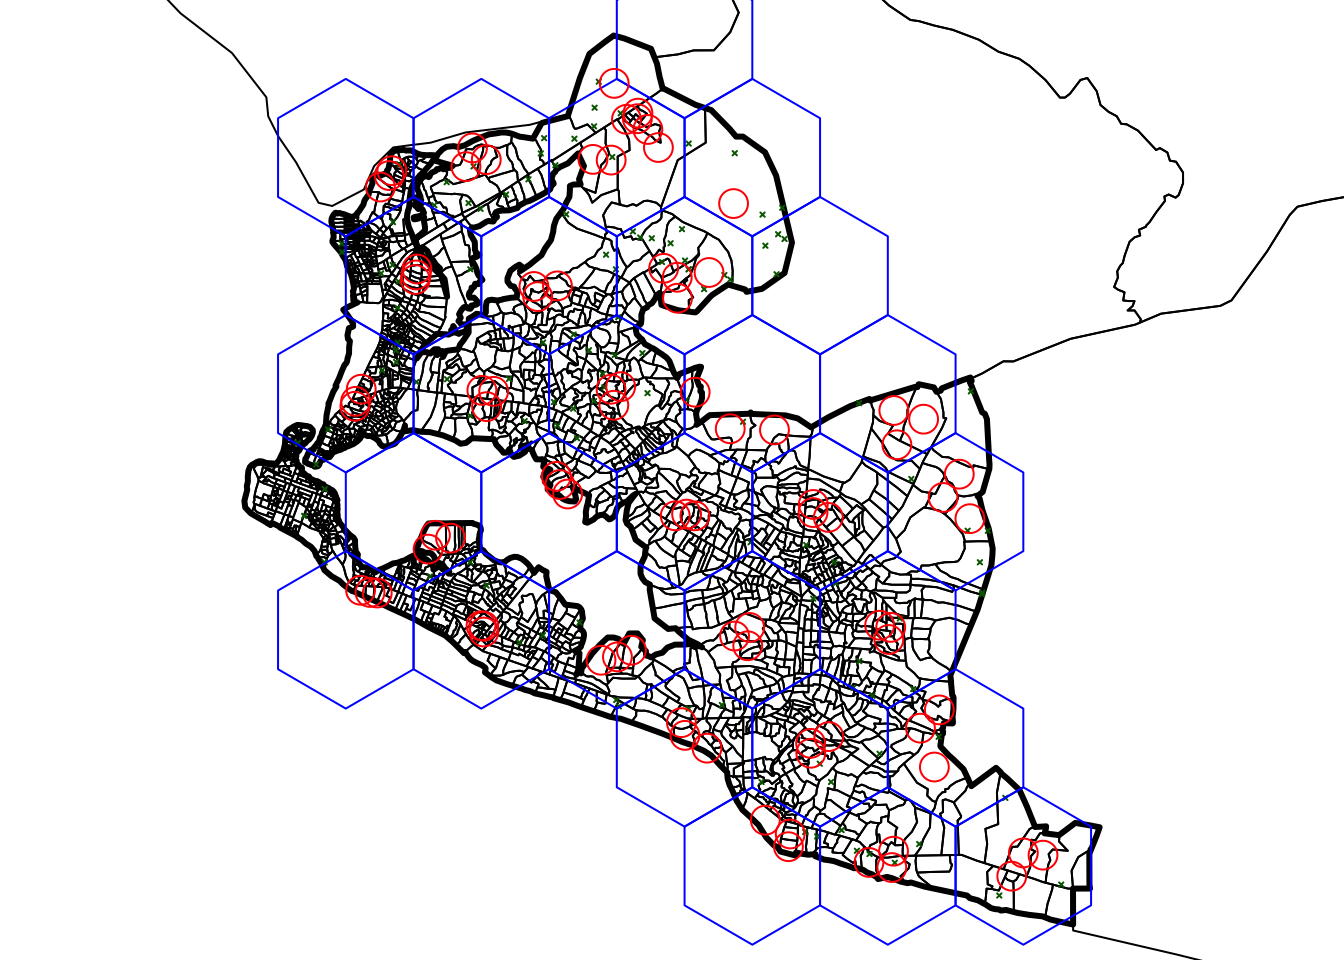
\includegraphics{figures/sample24-1} \hfill{}

\caption{Selected sampling points in Greater Monrovia District}\label{fig:sample24}
\end{figure}

~

The list of selected enumeration areas in Greater Monrovia is below:

~

~

\BeginKnitrBlock{rmddownload}
Download the list of selected enumeration areas in Greater Monrovia
District \href{data/greaterMonroviaSPlist.csv}{here}.
\EndKnitrBlock{rmddownload}

~

The stage 1 sample for Grand Bassa can be selected as follows:

~

\begin{figure}[H]

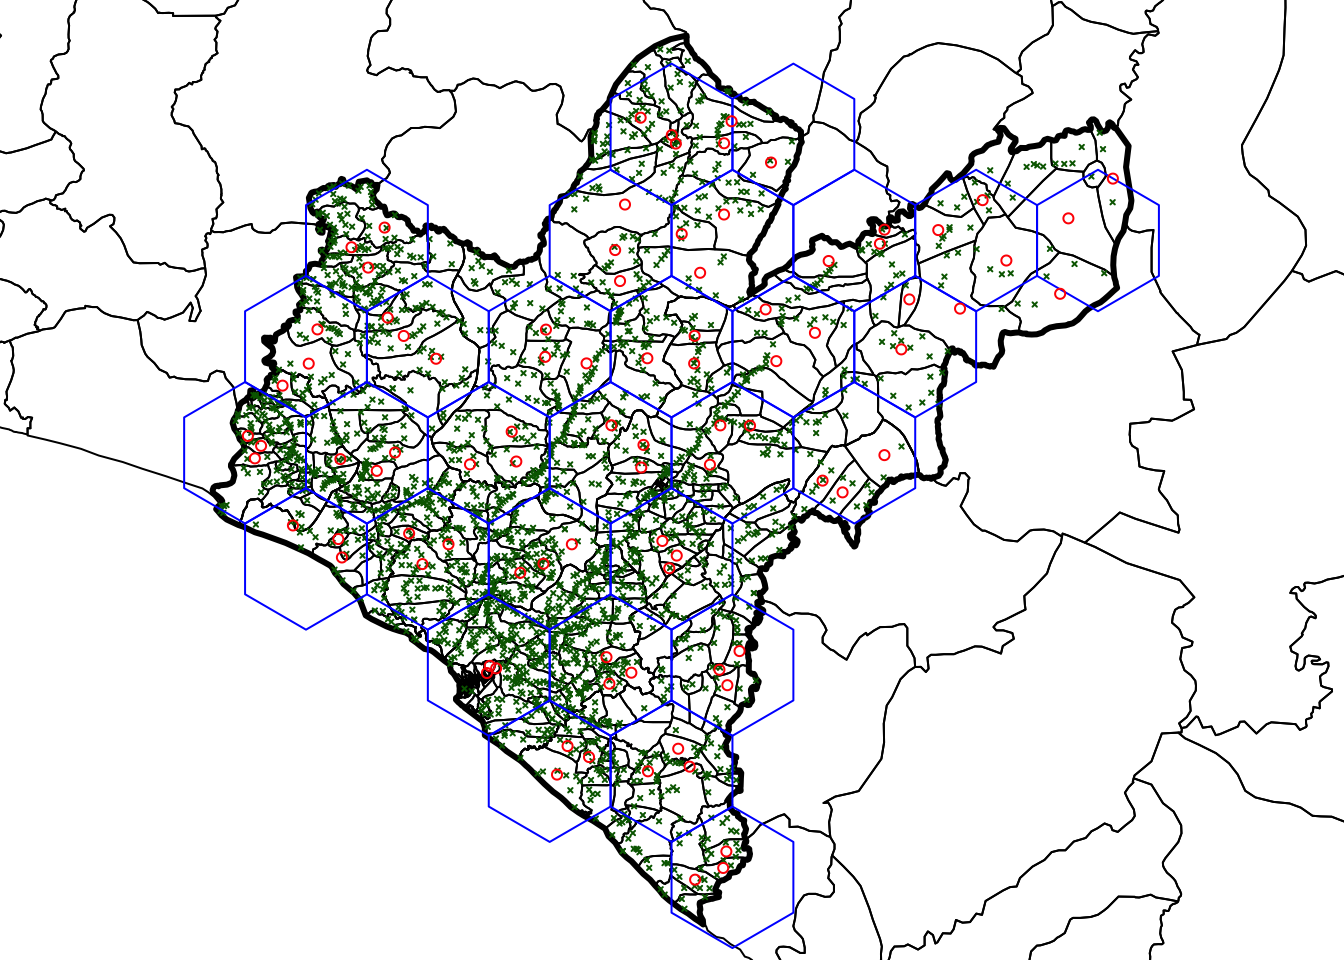
\includegraphics{figures/sample25-1} \hfill{}

\caption{Selected sampling points in Grand Bassa County}\label{fig:sample25}
\end{figure}

~

The list of selected sampling points in Grand Bassa is below:

~

~

\BeginKnitrBlock{rmddownload}
Download the list of selected enumeration areas in Grand Bassa County
\href{data/grandBassaSPlist.csv}{here}.
\EndKnitrBlock{rmddownload}

~

\hypertarget{sampling-frame-for-survey-of-children-aged-6-59-months-and-their-mothers}{%
\subsection{Sampling frame for survey of children aged 6-59 months and
their
mothers}\label{sampling-frame-for-survey-of-children-aged-6-59-months-and-their-mothers}}

Given a target sample size of 576 and using a stage 1 sample of 30 grids
as described above, a single nearest village to each of the 30 sampling
points identified in the stage 1 sample will be selected. In each of
these villages, the number of children 6-59 months and their mothers can
be estimated as follows:

~

\[\begin{aligned} 
n_{\text{children 6-59 months and mothers}} & ~ = ~ \left \lceil \frac{\text{Target sample size}}{\text{Number of villages}} \right \rceil \\
\\
& ~ = ~ \frac{576}{30} ~ \approx ~ 20
\end{aligned}\]

~

Twenty children 6-59 months and their mothers will need to be sampled
from each of the first villages of the 30 sampling points for each
county (and urban areas if included).

This will mean that the sampling interval to use for the door/house
counting with systematic selection for the stage 2 sampling of the
survey for children 6-59 months and their mothers can be calculated as
follows:

~

\[\begin{aligned}
n_{\text{Sampling interval}} & ~ = ~ \frac{\text{Total number of houses/doors}}{\text{Target sample of children 6-59 months old in village}} \\
\\
& ~ = ~ \frac{\text{Total number of houses/doors}}{\text{20}}
\end{aligned}\]

\newpage

\hypertarget{estimated-time-to-complete-full-survey}{%
\section{Estimated time to complete full
survey}\label{estimated-time-to-complete-full-survey}}

Given the overall sampling frame for SAM coverage survey and survey for
children 6-59 months and their mothers, the estimated time to complete
the whole survey will be based on the total number of villages to sample
and based on an assumed/estimated rate of completion of a single village
by single survey team.

A total of 90 villages will need to be sampled per county (and per urban
area if included). Assuming that a single survey team can enumerate one
village in a day, then the following lent of survey in days can be
considered based on number of survey teams:

~

\begin{longtable}[]{@{}lccc@{}}
\caption{\label{tab:surveydays} Estimated length of full survey in days
given number of survey teams and number of areas to
survey}\tabularnewline
\toprule
\begin{minipage}[b]{0.24\columnwidth}\raggedright
\textbf{Number of survey teams}\strut
\end{minipage} & \begin{minipage}[b]{0.24\columnwidth}\centering
\textbf{Length of survey}

(per county/area)\strut
\end{minipage} & \begin{minipage}[b]{0.24\columnwidth}\centering
\textbf{Length of survey}

(2 counties)\strut
\end{minipage} & \begin{minipage}[b]{0.24\columnwidth}\centering
\textbf{Length of survey}

(2 rural, 1 urban)\strut
\end{minipage}\tabularnewline
\midrule
\endfirsthead
\toprule
\begin{minipage}[b]{0.24\columnwidth}\raggedright
\textbf{Number of survey teams}\strut
\end{minipage} & \begin{minipage}[b]{0.24\columnwidth}\centering
\textbf{Length of survey}

(per county/area)\strut
\end{minipage} & \begin{minipage}[b]{0.24\columnwidth}\centering
\textbf{Length of survey}

(2 counties)\strut
\end{minipage} & \begin{minipage}[b]{0.24\columnwidth}\centering
\textbf{Length of survey}

(2 rural, 1 urban)\strut
\end{minipage}\tabularnewline
\midrule
\endhead
\begin{minipage}[t]{0.27\columnwidth}\raggedright
5 survey teams\strut
\end{minipage} & \begin{minipage}[t]{0.20\columnwidth}\centering
18 days\strut
\end{minipage} & \begin{minipage}[t]{0.20\columnwidth}\centering
36 days\strut
\end{minipage} & \begin{minipage}[t]{0.20\columnwidth}\centering
54 days\strut
\end{minipage}\tabularnewline
\begin{minipage}[t]{0.27\columnwidth}\raggedright
10 survey teams\strut
\end{minipage} & \begin{minipage}[t]{0.20\columnwidth}\centering
10 days\strut
\end{minipage} & \begin{minipage}[t]{0.20\columnwidth}\centering
20 days\strut
\end{minipage} & \begin{minipage}[t]{0.20\columnwidth}\centering
30 days\strut
\end{minipage}\tabularnewline
\begin{minipage}[t]{0.27\columnwidth}\raggedright
15 survey teams\strut
\end{minipage} & \begin{minipage}[t]{0.20\columnwidth}\centering
6 days\strut
\end{minipage} & \begin{minipage}[t]{0.20\columnwidth}\centering
12 days\strut
\end{minipage} & \begin{minipage}[t]{0.20\columnwidth}\centering
18 days\strut
\end{minipage}\tabularnewline
\bottomrule
\end{longtable}

~

\hypertarget{indicators}{%
\chapter{Indicators}\label{indicators}}

\hypertarget{cmam-coverage}{%
\section{CMAM coverage}\label{cmam-coverage}}

CMAM coverage usually pertains to coverage of SAM treatment.
Historically, there have been two coverage estimators in common use:
\textbf{point} and \textbf{period} coverage.

Point coverage is the number of current SAM cases in a treatment
programme divided by the total number of current SAM cases.

\textbf{Point coverage} uses data for current cases only. It is
calculated using the following formula:

\$nbsp;

\[\begin{aligned} 
\text{Point coverage} & ~ = ~ \frac{C_{in}}{C_{in} ~ + ~ C_{out}} \\
\\
where: & \\
\\
C_{in} & ~ = ~ \text{current SAM cases in the programme} \\
C_{out} & ~ = ~ \text{current SAM cases out of the programme}
\end{aligned}\]

~

\textbf{Point coverage} provides a snapshot of programme performance,
putting a strong emphasis on the effectiveness and timeliness of
case-finding and recruitment \citep{Myatt:2012tt}.

\textbf{Period coverage}, on the other hand, uses data for both current
and recovering cases. It is calculated using the following formula:

~

\[\begin{aligned}
\text{Period coverage} & ~ = ~ \frac{C_{in} ~ + ~ R_{in}}{C_{in} ~ + ~ C_{out} ~ + ~ R_{in}} \\
\\
where: & \\
\\
R_{in} & ~ = ~ \text{recovering SAM cases in the programme}
\end{aligned}\]

~

\textbf{Period coverage} is the number of current and recovering cases
in a treatment programme divided by all current SAM cases and recovering
cases. It approximates treatment coverage much better (albeit with
limitations) as it accounts for children who are no longer cases but are
in the programme.

Point and period coverage both have their limitations.

Point coverage of a programme with good case-finding and recruitment and
short lengths of stay can be misleadingly low because there are too few
current cases. For example, a coverage survey found:

~

\begin{longtable}[]{@{}rr@{}}
\caption{\label{tab:survey1} Scenario 1 - coverage survey results from a
programme with good case-finding and recruitment and short lengths of
stay}\tabularnewline
\toprule
\begin{minipage}[t]{0.43\columnwidth}\raggedleft
Number of current cases\strut
\end{minipage} & \begin{minipage}[t]{0.08\columnwidth}\raggedleft
2\strut
\end{minipage}\tabularnewline
\begin{minipage}[t]{0.43\columnwidth}\raggedleft
Number of current cases in the programme\strut
\end{minipage} & \begin{minipage}[t]{0.08\columnwidth}\raggedleft
0\strut
\end{minipage}\tabularnewline
\begin{minipage}[t]{0.43\columnwidth}\raggedleft
Number of current cases not in the programme\strut
\end{minipage} & \begin{minipage}[t]{0.08\columnwidth}\raggedleft
2\strut
\end{minipage}\tabularnewline
\begin{minipage}[t]{0.43\columnwidth}\raggedleft
Number of recovering cases in the programme\strut
\end{minipage} & \begin{minipage}[t]{0.08\columnwidth}\raggedleft
34\strut
\end{minipage}\tabularnewline
\bottomrule
\end{longtable}

~

In this scenario, the point coverage estimator returns:

~

\[ \text{Point coverage} ~ = ~ \frac{C_{in}}{C_{out}} ~ = ~ \frac{0}{2} ~ = ~ 0 ~ = ~ 0\% \]

~

but the period estimator returns:

~

\[ \text{Period coverage} ~ = ~ \frac{0 ~ + ~ 34}{0 ~ + ~ 34 ~ + ~ 2} ~ = ~ 0.944 ~ = ~ 94.4\% \]

~

In this regard, the point coverage estimate penalises good performance
and the period coverage most likely better depicts the coverage of the
programme.

On the other hand, a programme with poor case-finding and recruitment
and long lengths of stay due to late presentation and/or late admission
may have a period coverage that is misleadingly high because of high
number of recovering cases. In such a scenario, the two estimators will
yield very different results. For example:

~

\begin{longtable}[]{@{}rr@{}}
\caption{\label{tab:survey1} Scenario 2 - coverage survey results from a
programme with good case-finding and recruitment and short lengths of
stay}\tabularnewline
\toprule
\begin{minipage}[t]{0.43\columnwidth}\raggedleft
Number of current cases\strut
\end{minipage} & \begin{minipage}[t]{0.08\columnwidth}\raggedleft
12\strut
\end{minipage}\tabularnewline
\begin{minipage}[t]{0.43\columnwidth}\raggedleft
Number of current cases in the programme\strut
\end{minipage} & \begin{minipage}[t]{0.08\columnwidth}\raggedleft
3\strut
\end{minipage}\tabularnewline
\begin{minipage}[t]{0.43\columnwidth}\raggedleft
Number of current cases not in the programme\strut
\end{minipage} & \begin{minipage}[t]{0.08\columnwidth}\raggedleft
9\strut
\end{minipage}\tabularnewline
\begin{minipage}[t]{0.43\columnwidth}\raggedleft
Number of recovering cases in the programme\strut
\end{minipage} & \begin{minipage}[t]{0.08\columnwidth}\raggedleft
22\strut
\end{minipage}\tabularnewline
\bottomrule
\end{longtable}

~

\[ \text{Point coverage} ~ = ~ \frac{C_{in}}{C_{out}} ~ = ~ \frac{3}{12} ~ = ~ 0.250 ~ = ~ 25.0\% \]

~

but the period estimator returns:

~

\[ \text{Period coverage} ~ = ~ \frac{3 ~ + ~ 22}{3 ~ + ~ 22 ~ + ~ 9} ~ = ~ 0.735 ~ = ~ 73.5\% \]

~

In this example, point coverage is the more reflective coverage of the
programme.

It should be noted also that period coverage has a tendency to an
overestimation bias. This is because the current period coverage
estimator does not take into account cases of acute malnutrition who
have recovered spontaneously but were never enrolled in any treatment
programme.

An estimator of coverage that does include both recovering cases that
are in the programme and recovering cases that are not in the programme
and, thus, provides an unbiased estimator of overall programme
performance is:

~

\[\begin{aligned}
\text{Single coverage} & ~ = ~ \frac{C_{in} ~ + ~ R_{in}}{C_{in} ~ + ~ R_{in} ~ + ~ C_{out} ~ + ~ R_{out}} \\
\\
where: & \\
\\
R_{out} & ~ = ~ \text{Recovering SAM cases not in the programme}
\end{aligned}\]

~

It is for these reasons that the coverage assessment technical guide
\citep{Myatt:2012tt} recommends that only one of these estimators be
reported and the choice of estimator to report should be guided by
specific programme features and characteristics (such as lengths of stay
in the programme) that would justify the choice of reported estimator.
In a recent Epicentre review \citep{Epicentre:2015ty} this has been
highlighted as a source of confusion and issues given the possibility of
period coverage being chosen more as a coverage estimator rather than
point coverage because of it being a higher estimate even if the
programme characteristics do not merit its use. The review suggests that
both coverage indicators could be reported, with sufficient context
(e.g.~on length of stay, timeliness of admissions, etc.) to allow for
their interpretation.

In response to the review and to address the limitations of the coverage
estimators, development work has been conducted on further developing
and improving the coverage estimators to address this confusion and the
issues around them \citep{Balegamire:2015ud}. This work focused
primarily on improving the period coverage estimator to address the
overestimation bias described earlier and to make it more closely
approximate the treatment coverage estimator formula shown above.

The problem with this estimator is that \(R_{out}\) (i.e.~the number of
recovering cases that are not in the programme) is unknown and may be
difficult to collect accurately. This problem of estimating the number
of recovering cases not in the programme (\(R_{out}\)) may be addressed
using a simple mathematical model\footnote{This model assumes that
  incidence of acute malnutrition and programme coverage do not vary
  rapidly over time.} proposed by \citet{Balegamire:2015ud}.

~

\[\begin{aligned}
\frac{C_{in} ~ + ~ C_{out}}{C_{in}} & ~ \approx ~ \frac{R_{in} ~ + ~ k ~ \times ~ R_{out}}{R_{in}} \\
\\
where: & \\
\\
k & ~ = ~ \text{a correction factor}
\end{aligned}\]

~

\(R_{out}\) can then be expressed in terms of the known variables:

~

\[  R_{out} ~ \approx ~ \left \lfloor ~ \frac{1}{k} ~ \times ~ \left ( ~ R_{in} ~ \times ~ \frac{C_{in} ~ + ~ C_{out}}{C_{in}} ~ - ~ R_{in} ~ \right ) ~ \right \rfloor \]

~

Given the possibility that no cases in the programme (\(C_{in}\)) are
found, the calculation is adjusted by adding 1 to \(C_{in}\). To arrive
at a whole number value for \(R_{out}\), the calculation is rounded off
towards zero.

~

\[ R_{out} ~ \approx ~ \left \lfloor ~ \frac{1}{k} ~ \times ~ \left ( ~ R_{in} ~ \times ~ \frac{C_{in} ~ + ~ 1 ~ + ~ C_{out}}{C_{in} ~ + ~ 1} ~ - ~ R_{in} ~ \right ) ~ \right \rfloor \]

~

This leaves the problem of deciding a suitable value for the correction
factor (\(k\)). A reasonable candidate for \(k\) is the ratio of the
mean length of an untreated episode to the mean length of a CMAM
treatment episode.

~

\[ k ~ = ~ \frac{\text{Mean length of untreated episode}}{\text{Mean length of a treatment episode}} \]

~

Possible value for mean length of untreated episode is 7.5 months
\citep{Garenne:2009fq} which is the common value used when estimating
programme case-loads from prevalence estimates \citep{Myatt:2012tu}.
Mean length of a treatment episode can be estimated by calculating the
mean length of stay in the CMAM programme using routine monitoring data.
In general, A value of 2.5 months could be used in the absence of better
information or when the validity of routine programme monitoring data is
suspect. Using these values, k is:

~

\[ k ~ = ~ \frac{\text{Mean length of untreated episode}}{\text{Mean length of a treatment episode}} ~ = ~ \frac{7.5}{2.5} ~ = ~ 3 \]

~

The inclusion of recovering cases means that the single coverage
estimate is mathematically constrained to return a coverage estimate
that is greater than or equal to the point coverage estimate. The
underestimation present in the point coverage estimate has, to some
extent, been corrected. The inclusion of recovering cases that are not
in the programme means that the single coverage estimator is
mathematically constrained to return a coverage estimate that is less
than or equal to the period coverage estimate. The overestimation
present in the period coverage estimate has, to some extent, been
corrected.

Given this single coverage estimator, a shift in terminology is proposed
that is more descriptive and specific with regard to what the estimator
is actually measuring, allowing both measures to be reported together
without confusion. \textbf{Point coverage} is now named
\emph{case-finding effectiveness} to more precisely reflect it as a
measure of the programme's ability to find and recruit current cases.
This indicator assesses how good the treatment programme is in finding
cases of SAM and then getting them to treatment. \textbf{Period
coverage} that has been improved into the single coverage metric is now
named \emph{treatment coverage} as this is the estimator that
approximates this coverage indicator the closest.

\hypertarget{requirements}{%
\subsection{Requirements}\label{requirements}}

This indicator will require additional programmatic information to be
operationalised specific for Liberia.

It would be ideal that a Liberia-specific value for mean length of a
treatment episode be estimated using routine programme data from a
selection of cured cases from a selection of health centres providing
CMAM services in the two counties in which the survey is to be
implemented. This data should be collected from the beneficiary cards of
cured cases. For each county, a total of 30 health centres from the full
list of health centres in the county can be selected systematically. Of
these 30 health centres, a sample of 30 records of discharged cured
cases should be selected. From these records, data on date of admission
and date of discharge should be extracted collated into a data format
(ideally a comma-separated value or CSV file) with each of these values
in a separate column.

This data will allow the calculation of the mean length of stay in the
CMAM programme of discharge cured cases.

~

\[ \text{Mean length of stay} ~ = ~ \frac{\text{Length of stay in programme (days)}}{\text{Number of records}} \]

~

For data collection, enumerators will require:

\begin{enumerate}
\def\labelenumi{\arabic{enumi}.}
\item
  A height board;
\item
  A digital weighing scale; and,
\item
  A MUAC tape.
\end{enumerate}

Traditionally, if data collection is done using pen and paper,
enumerators are provided with z-score tables for weight-for-height so
that they can determine if child is SAM. Since this survey will utilise
digital data collection (see Section \ref{data}), the digital form will
determine whether the child is SAM by MUAC and/or weight-for-height
and/or oedema and will instruct the enumerators on what to do next if
the child is a SAM case.

Referral slips will also be needed so that children who are identified
as SAM but not in the programme can be referred.

\hypertarget{vitamin-a-supplementation}{%
\section{Vitamin A supplementation}\label{vitamin-a-supplementation}}

The standard estimator for vitamin A supplementation is the proportion
of children aged 6-59 months who received two age-appropriate doses of
vitamin A in the past 12 months.

In standard surveys such as the DHS and MICS, this indicator is adjusted
to a recall of 6 months for a single age-appropriate dose of vitamin A.

In order to determine whether supplementation with vitamin A is age
appropriate, vitamin A supplementation should first be assessed on the
child's health card. Provision of vitamin A card is usually recorded on
the child's health card with the corresponding does given. If health
card not available or if health card is lost or if the child doesn't
have a health card at all, then the mother/caregiver will have to be
asked whether their child has received vitamin A in the past 6 months
and respond by recall. If the mother/caregiver says yes, then the next
question to ask will be which type of gel capsule was provided. The blue
vitamin A gel capsule containing 100,000 IU of vitamin A is given to
children 6-11 months. The red vitamin A gel capsule containing 200,000
IU of vitamin A is given to children 12 - 59 months. A sample of the
blue and the red gel capsule (or a photo of the capsules) can be used to
aid the mother/caregiver in answering this question.

Given this, two indicators can be reported on vitamin A supplementation.

\begin{enumerate}
\def\labelenumi{\arabic{enumi}.}
\item
  Any vitamin A supplementation in the past 6 months.
\item
  Age-appropriate vitamin A supplementation in the past 6 months.
\end{enumerate}

\hypertarget{requirements-1}{%
\subsection{Requirements}\label{requirements-1}}

Either samples and/or photos of both the blue and red gel vitamin A
capsules will be needed per enumerator to use in aiding the mother to
answer which type of vitamin A gel capsule has been provided to the
child.

\hypertarget{iron-folic-acid-ifa-supplementation-for-pregnant-women}{%
\section{Iron-folic acid (IFA) supplementation for pregnant
women}\label{iron-folic-acid-ifa-supplementation-for-pregnant-women}}

Population-based surveys typically report the percentage of women with a
live birth in the two to five years before the survey who received and
took IFA supplementation during their most recent pregnancy. Because
antenatal care (ANC) is typically the main platform for IFA supplement
distribution for pregnant women, survey questions on antenatal care
attendance and timing of the first antenatal care visit can provide
information on the use of this platform to deliver IFA supplementation.
\citet{Sununtnasuk:2015kb} propose a falter point framework\footnote{Similar
  to a bottleneck framework and consistent with \citet{Tanahashi:1978we}
  hierarchical model of coverage.} that utilises four indicators that
proxy the four critical points at which the ANC approach to IFA
distribution might falter in IFA supplementation coverage to pregnant
women. These indicators are:

\begin{enumerate}
\def\labelenumi{\arabic{enumi}.}
\item
  At least one ANC visit during most recent pregnancy
\item
  Receipt or purchase of IFA tablet/s
\item
  IFA consumption
\item
  Adherence to 180 days of supplementation
\end{enumerate}

\hypertarget{requirements-2}{%
\subsection{Requirements}\label{requirements-2}}

It would be ideal for each enumerator to have a sample/s and/or photos
of an IFA tablet to show the respondent as an recall aid or prompt.
Given that some mothers may have to recall as far back as 5 years and
that they might not be able to remember that the tablet is called,
showing them a sample of the tablet might help them remember if they
have taken it.

\hypertarget{micronutrient-powder-supplementation}{%
\section{Micronutrient powder
supplementation}\label{micronutrient-powder-supplementation}}

The indicator for coverage of micronutrient powder supplementation is
the proportion of children aged 6-23 months who consume micronutrient
powder supplements. Depending on the programme protocol on mechanism of
distribution and effective intake of MNP, a full indicator set on MNP
supplementation can be devised that will be similar to the IFA
supplementation falter point or bottleneck framework. For example, if
MNPs were being provided through the health centres or health posts,
then the following indicators can be assessed hierarchically:

\begin{enumerate}
\def\labelenumi{\arabic{enumi}.}
\item
  Health centre / health post attendance in the past month
\item
  Awareness of MNP
\item
  Consumption of MNP
\end{enumerate}

\hypertarget{requirement}{%
\subsection{Requirement}\label{requirement}}

It would be ideal to provide enumerators with sample/s and/or photo/s of
MNP sachets used in Liberia. If there are various brands of MNP
distributed, it would be good to have sample/s and/or photo/s of each
one. These sample/s and/or photo/s can be used to help mothers or
caregivers recall or know what an MNP is and be able to ascertain
whether they do know it or have heard of it and whether their child has
consumed it.

\hypertarget{iycf-counselling}{%
\section{IYCF counselling}\label{iycf-counselling}}

There are no standard indicators for IYCF counselling. Any indicator
developed for this programme will depend on the mechanics of how the
IYCF counselling is delivered and who the target beneficiaries are. In
terms of mechanism, what is known so far is that these sessions are
delivered via the health clinic/health post and that the target
beneficiaries are pregnant women. Given this, similar approach to the
IFA supplementation coverage of falter points/bottle necks can be used
with the following indicators:

\begin{enumerate}
\def\labelenumi{\arabic{enumi}.}
\item
  At least one ANC visit during most recent pregnancy
\item
  Awareness of IYCF counselling (have they been advised IYCF counselling
  when they attended ANC)
\item
  Attendance to IYCF counselling
\end{enumerate}

\hypertarget{requirement-1}{%
\subsection{Requirement}\label{requirement-1}}

It would be ideal to have the training materials used for IYCF
counselling and the materials used when conducting IYCF counselling.
These materials can be used as a recall aid for mothers/caregivers who
are being asked about whether they know or have heard about IYCF
counselling and whether they have attended.

\hypertarget{questionnaire}{%
\chapter{Questionnaire}\label{questionnaire}}

The following are sample/template questionnaires used for the two types
of surveys that will be implemented.

\hypertarget{cmam-coverage-survey-instruments}{%
\section{CMAM coverage survey
instruments}\label{cmam-coverage-survey-instruments}}

CMAM coverage surveys use primarily use two forms. The first form is
used to collect coverage data from SAM children found during the survey.
Given that this survey will use house-to-house/door-to-door sampling for
stage 2, then it would be necessary to record all data from all children
that are measured with MUAC, weight-for-height and oedema. The following
tabular form can be used for this purpose:

\newpage

\begin{figure}[H]

{\centering 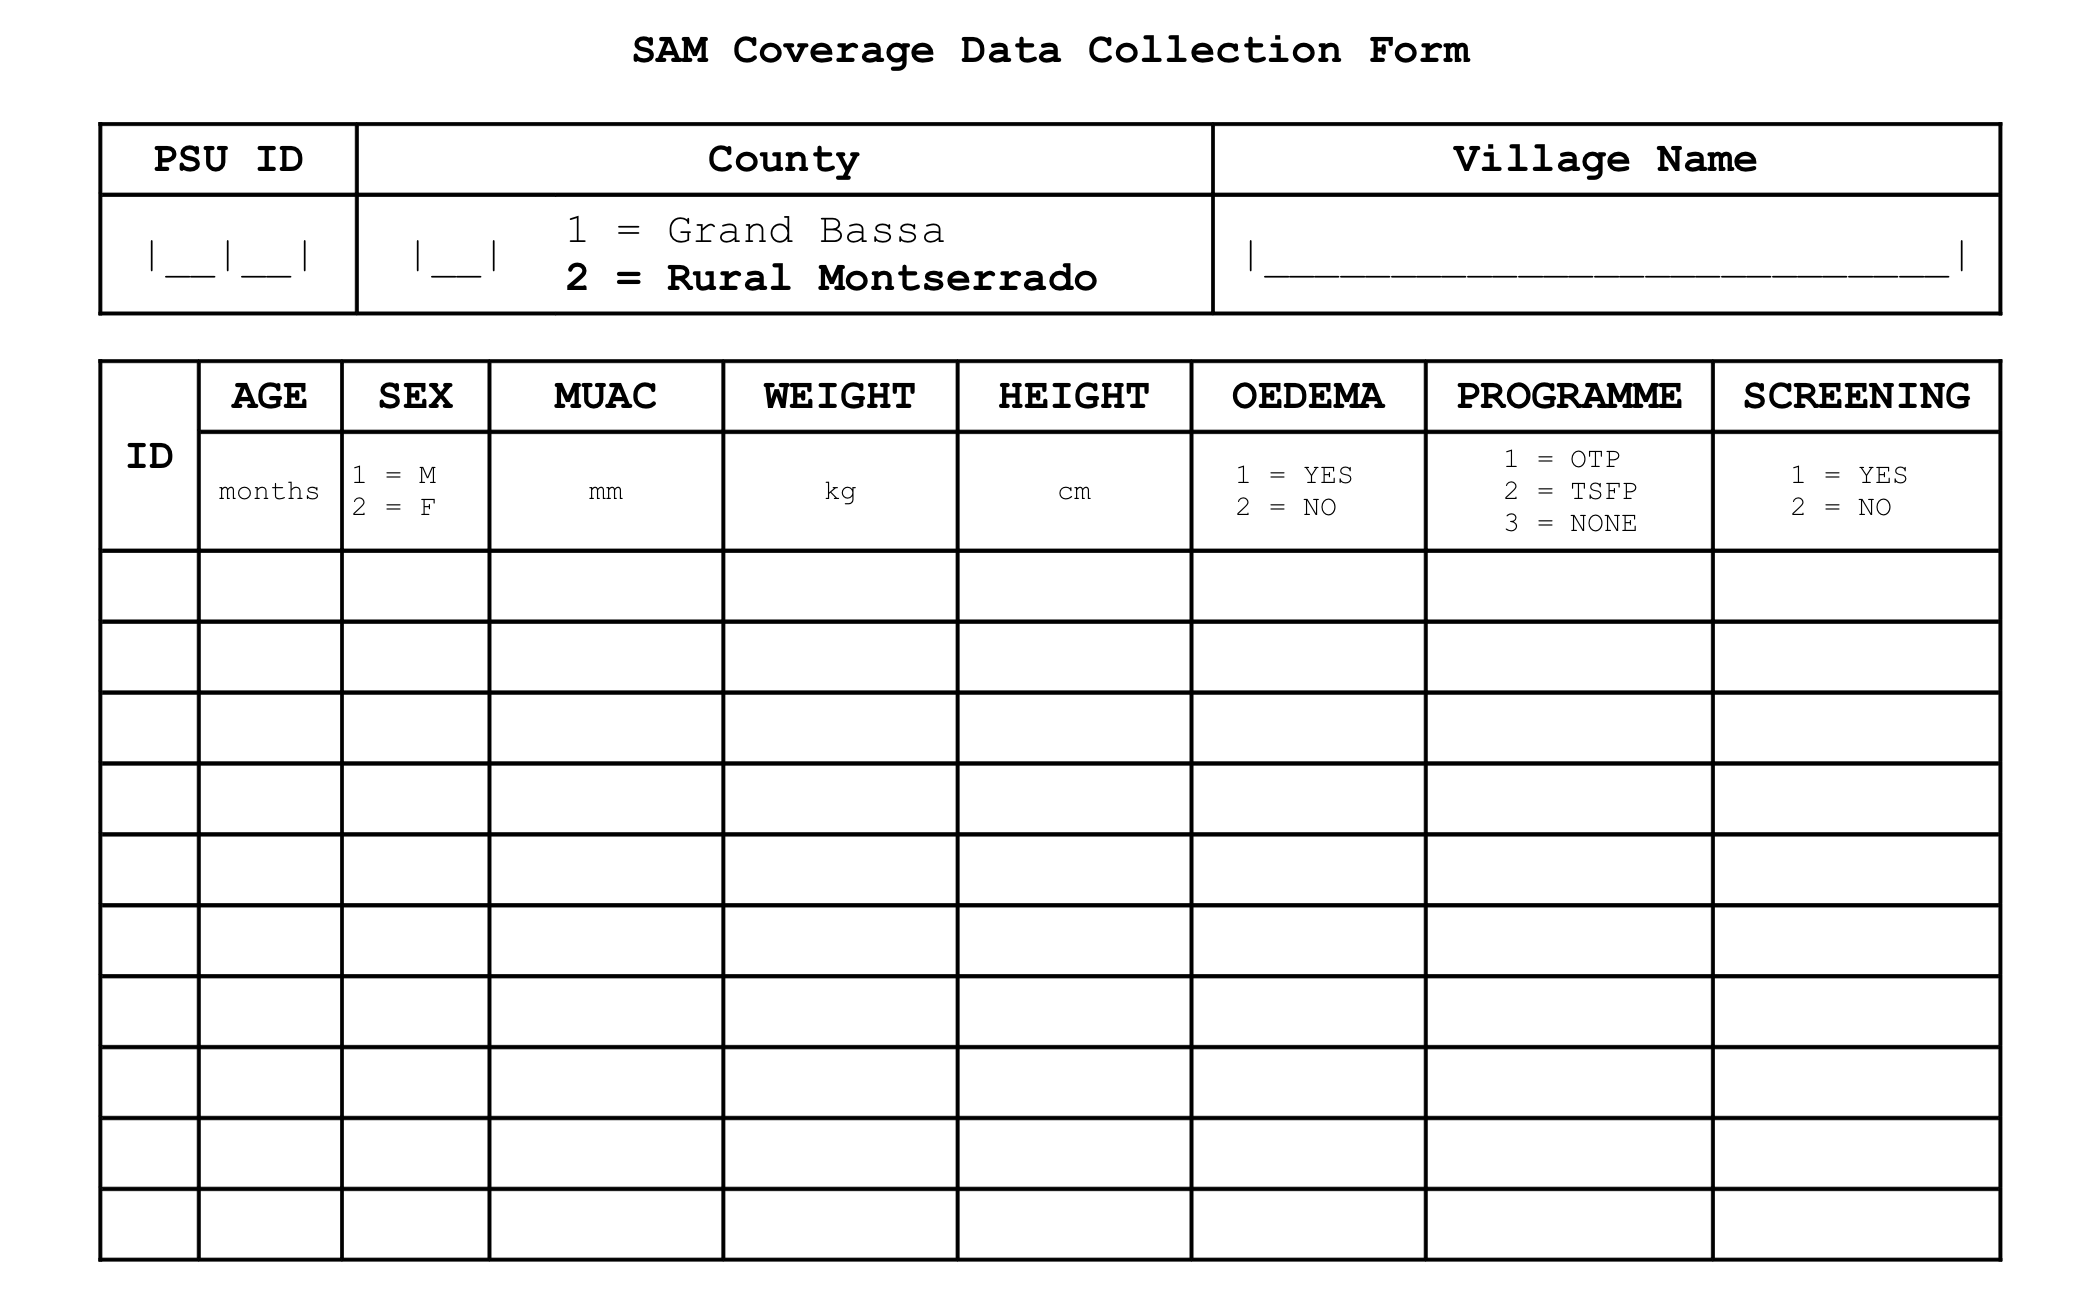
\includegraphics[width=0.9\linewidth]{forms/samForm} 

}

\caption{SAM coverage survey sample/template form}\label{fig:samform}
\end{figure}

~

The data collected using the tabular forms will allow estimation of
coverage. They do not, however, allow you to know the reasons for
coverage failure. To collect this data we apply a ``barriers''
questionnaire to the mothers/carers of uncovered SAM cases. Here is an
example of a barriers questionnaire:

\newpage

\begin{figure}[H]

{\centering 
\includegraphics[width=0.9\linewidth]{forms/samBarriersForm} 

}

\caption{SAM coverage barriers survey sample/template form}\label{fig:sambarriers}
\end{figure}

\newpage

\hypertarget{survey-for-children-6-59-months-and-their-mothers}{%
\section{Survey for children 6-59 months and their
mothers}\label{survey-for-children-6-59-months-and-their-mothers}}

For the survey for children 6-59 months, following is a sample/template
questionnaire.

\begin{figure}[H]

{\centering 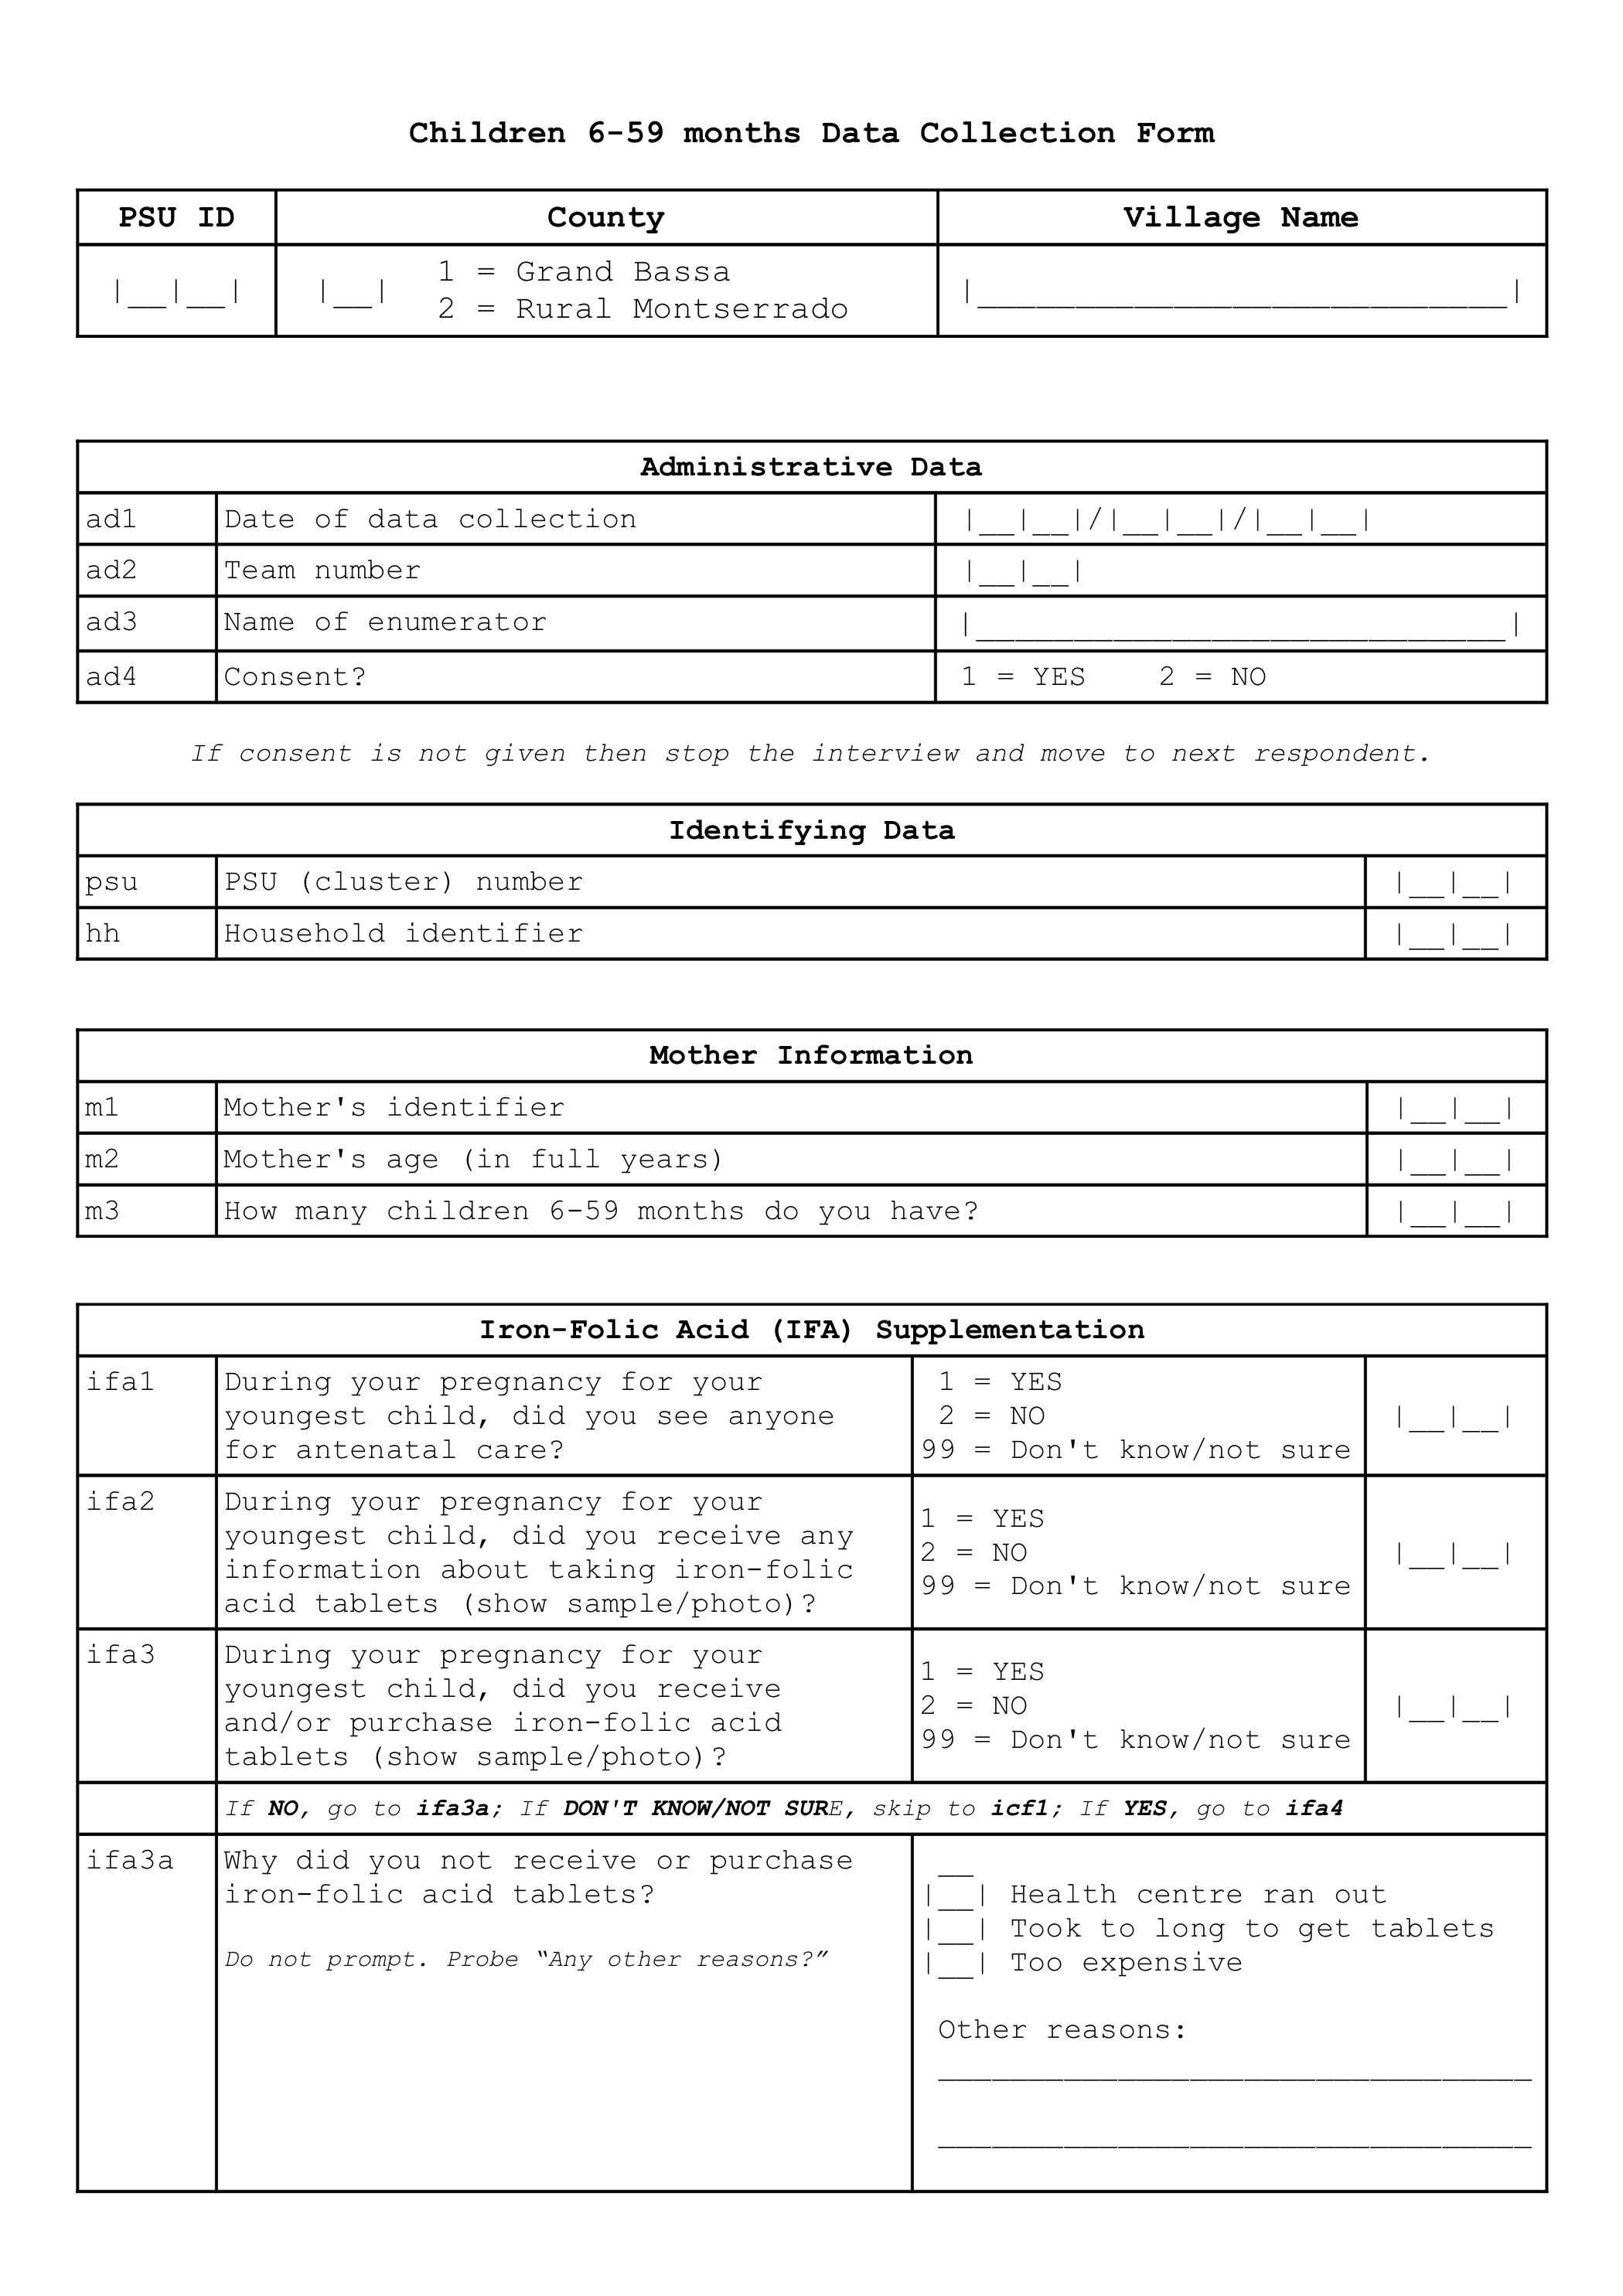
\includegraphics[width=0.9\linewidth]{forms/childForm1} 

}

\caption{Children 6-59 months old and their mothers survey sample/template form}\label{fig:childform1}
\end{figure}\begin{figure}[H]

{\centering 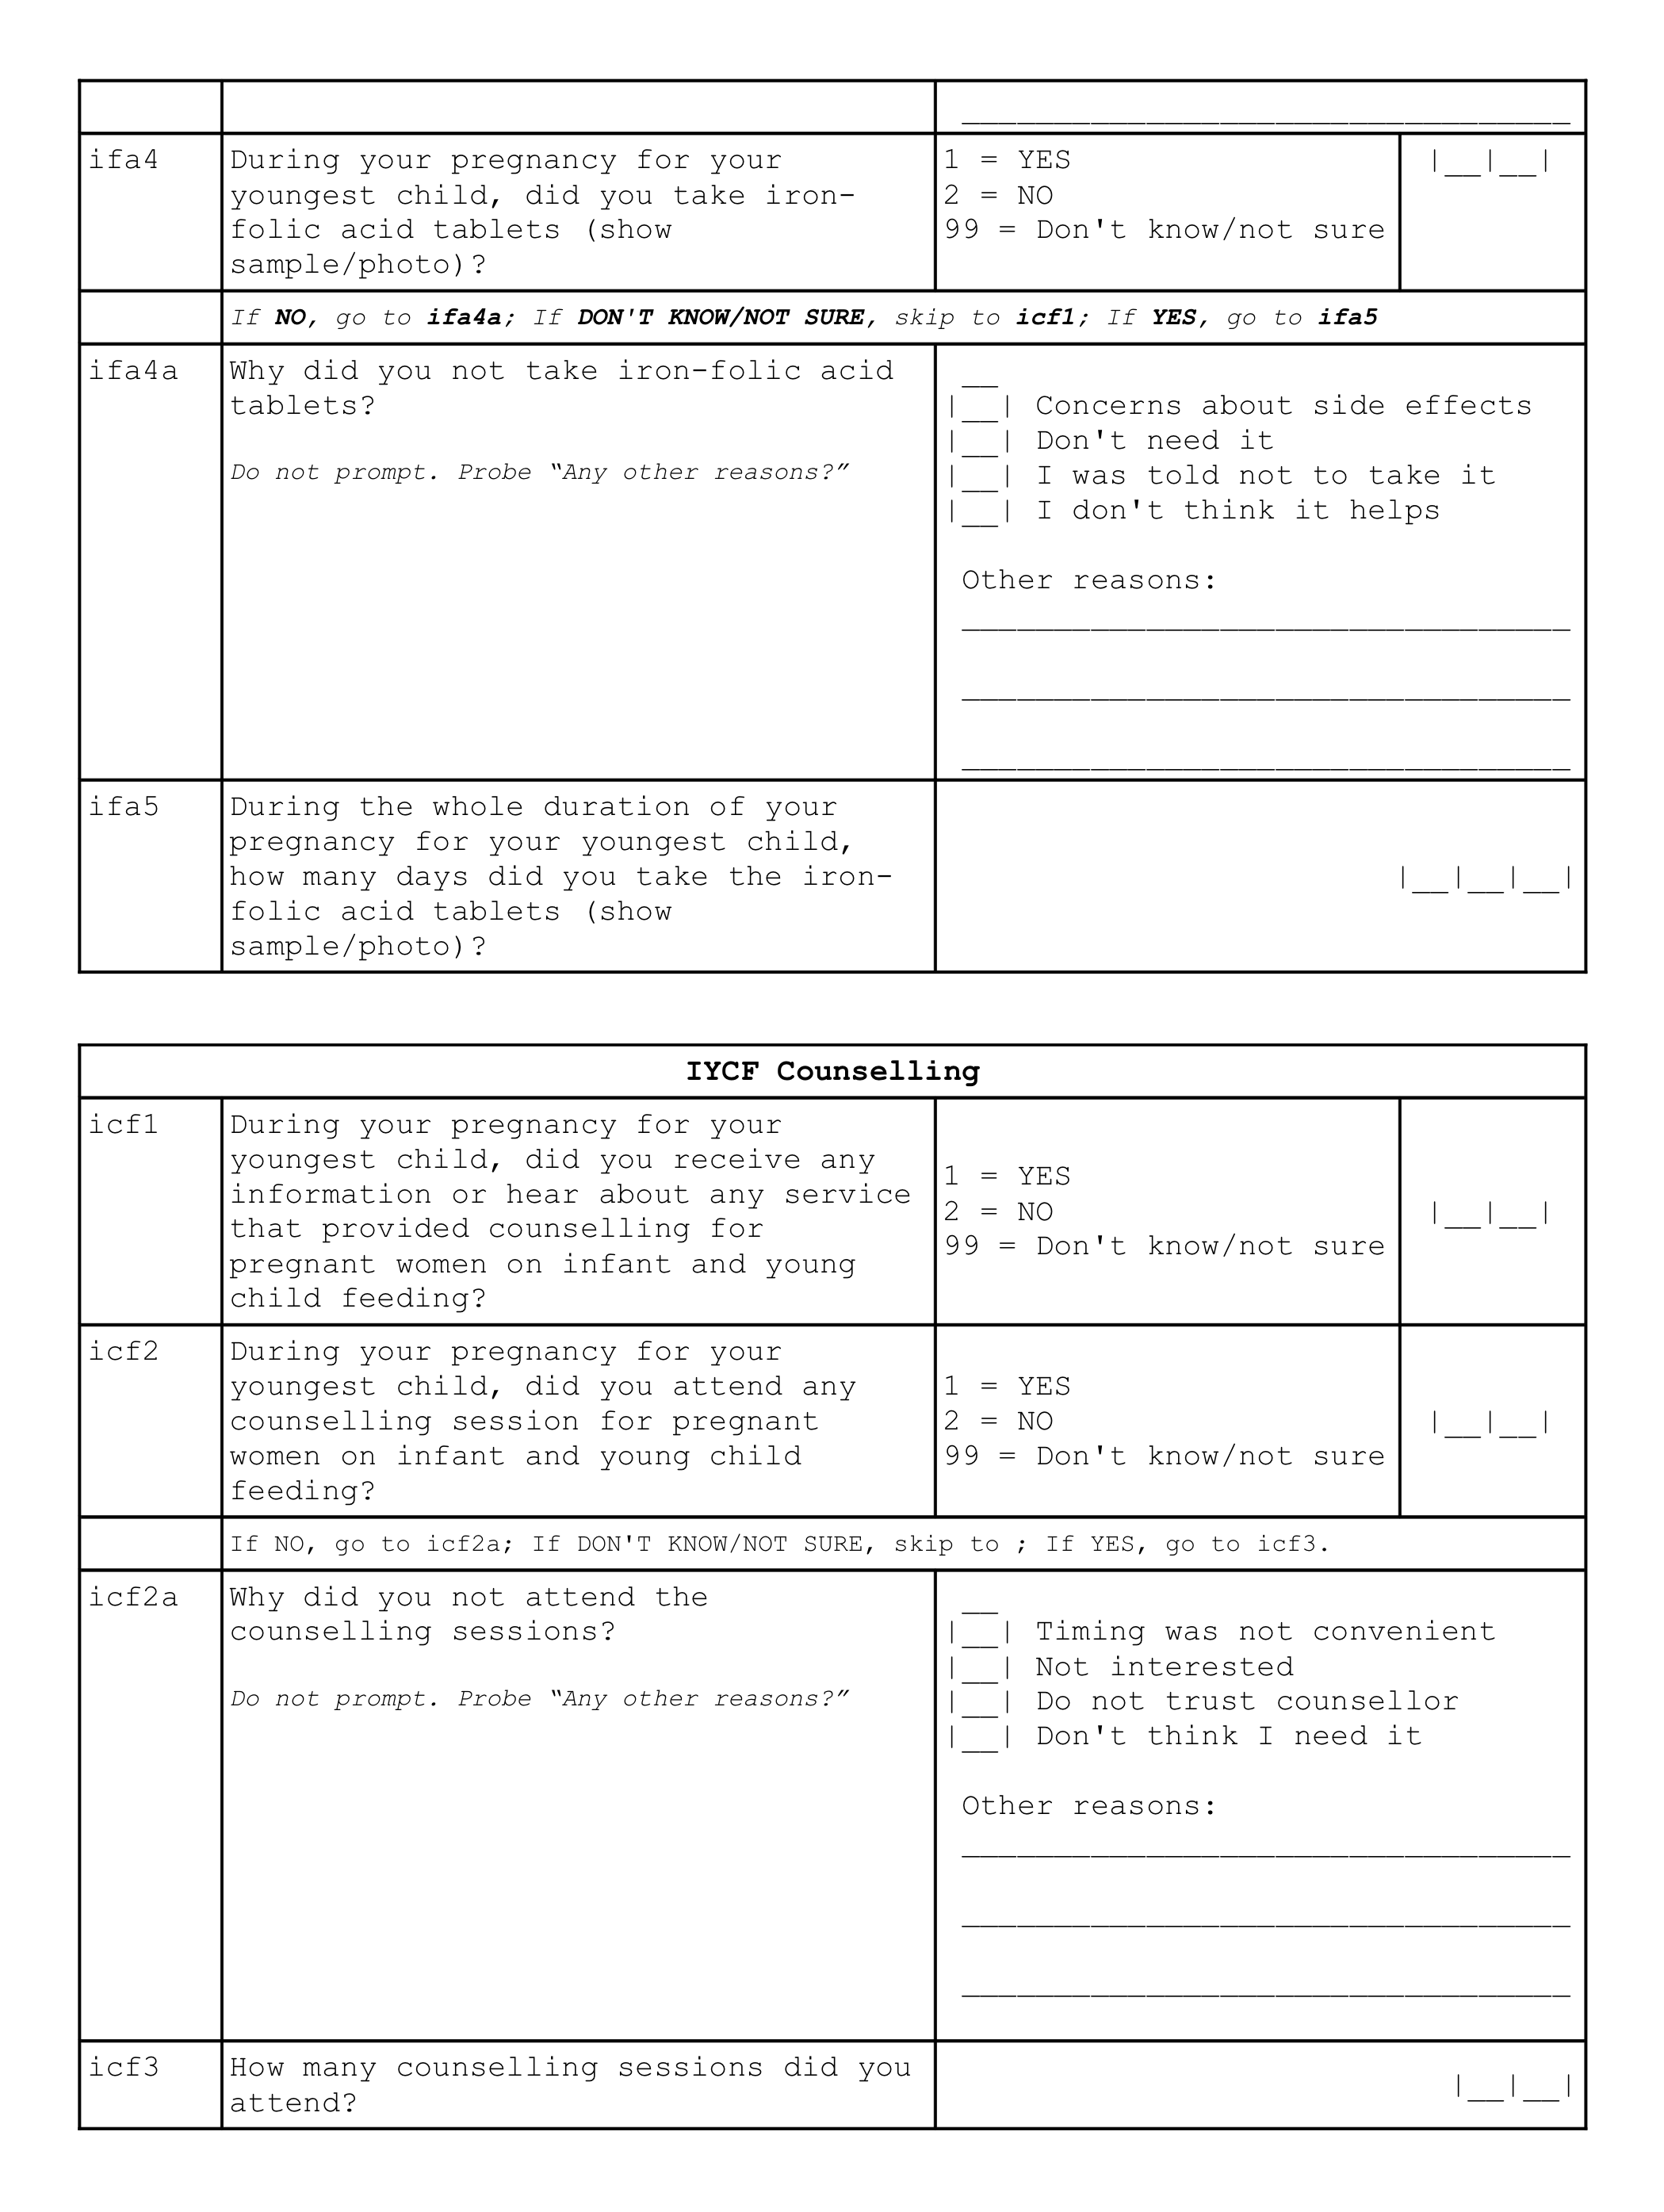
\includegraphics[width=0.9\linewidth]{forms/childForm2} 

}

\caption{Children 6-59 months old and their mothers survey sample/template form}\label{fig:childform1}
\end{figure}\begin{figure}[H]

{\centering 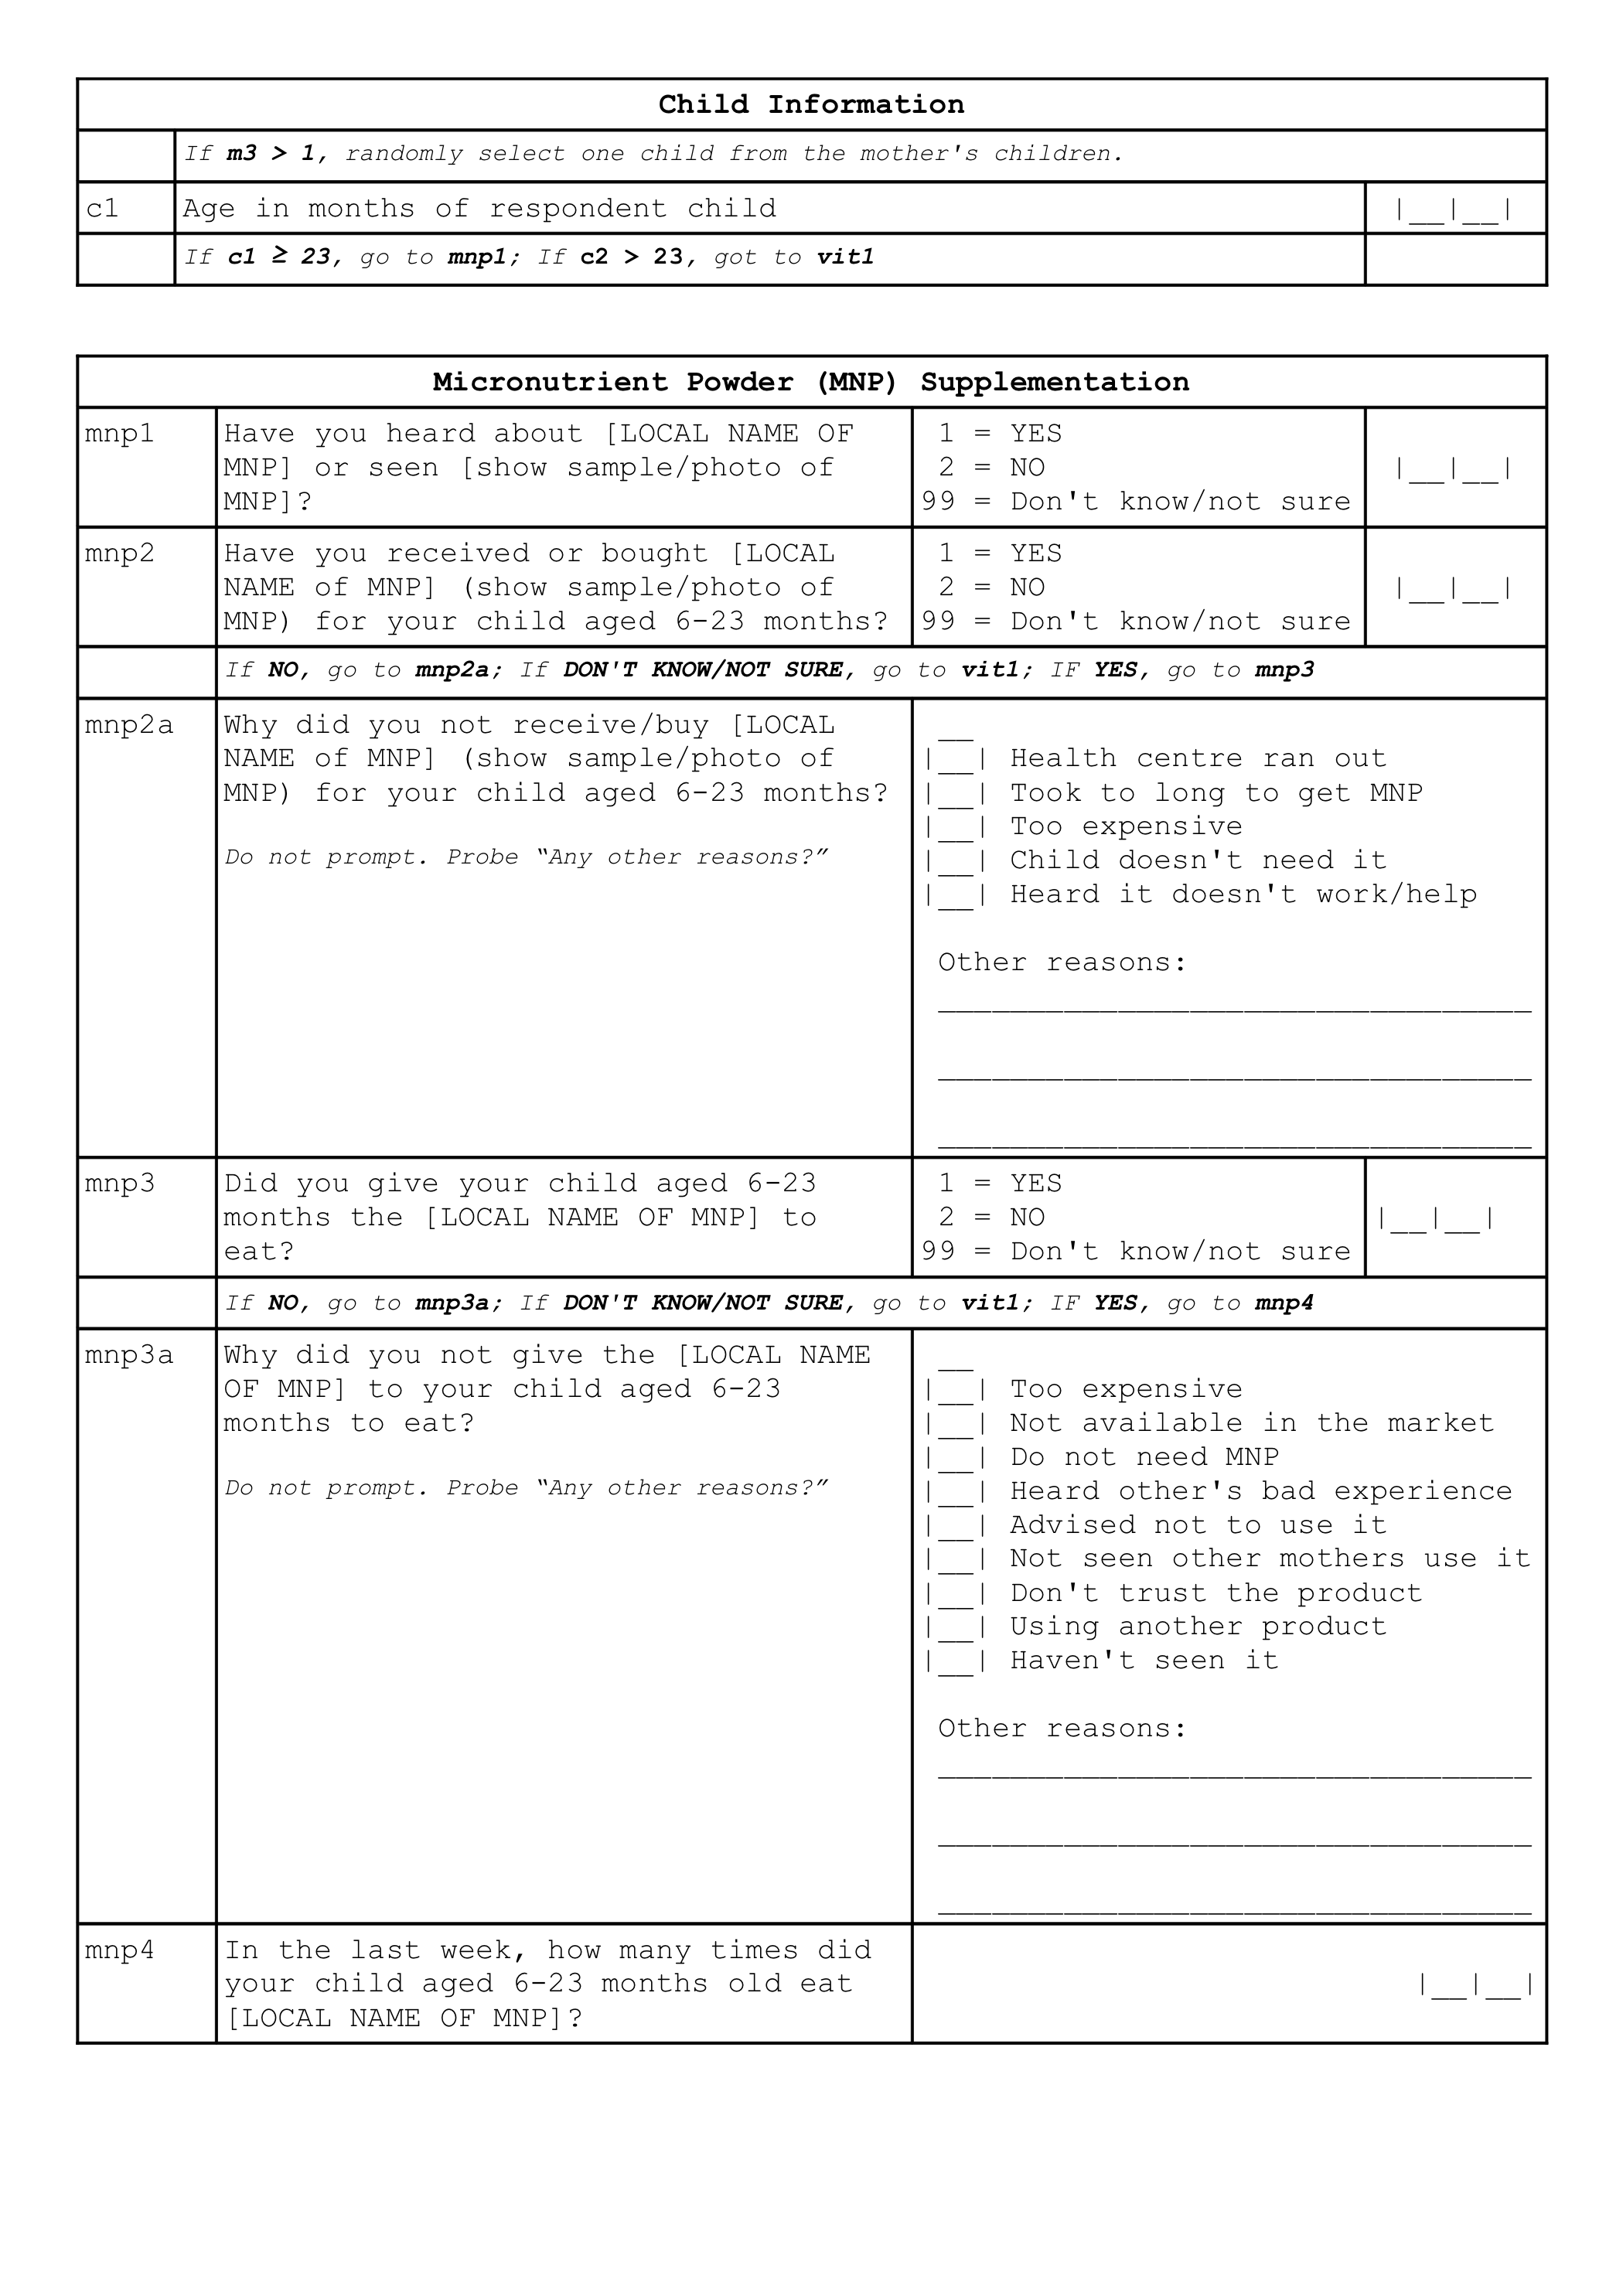
\includegraphics[width=0.9\linewidth]{forms/childForm3} 

}

\caption{Children 6-59 months old and their mothers survey sample/template form}\label{fig:childform1}
\end{figure}\begin{figure}[H]

{\centering 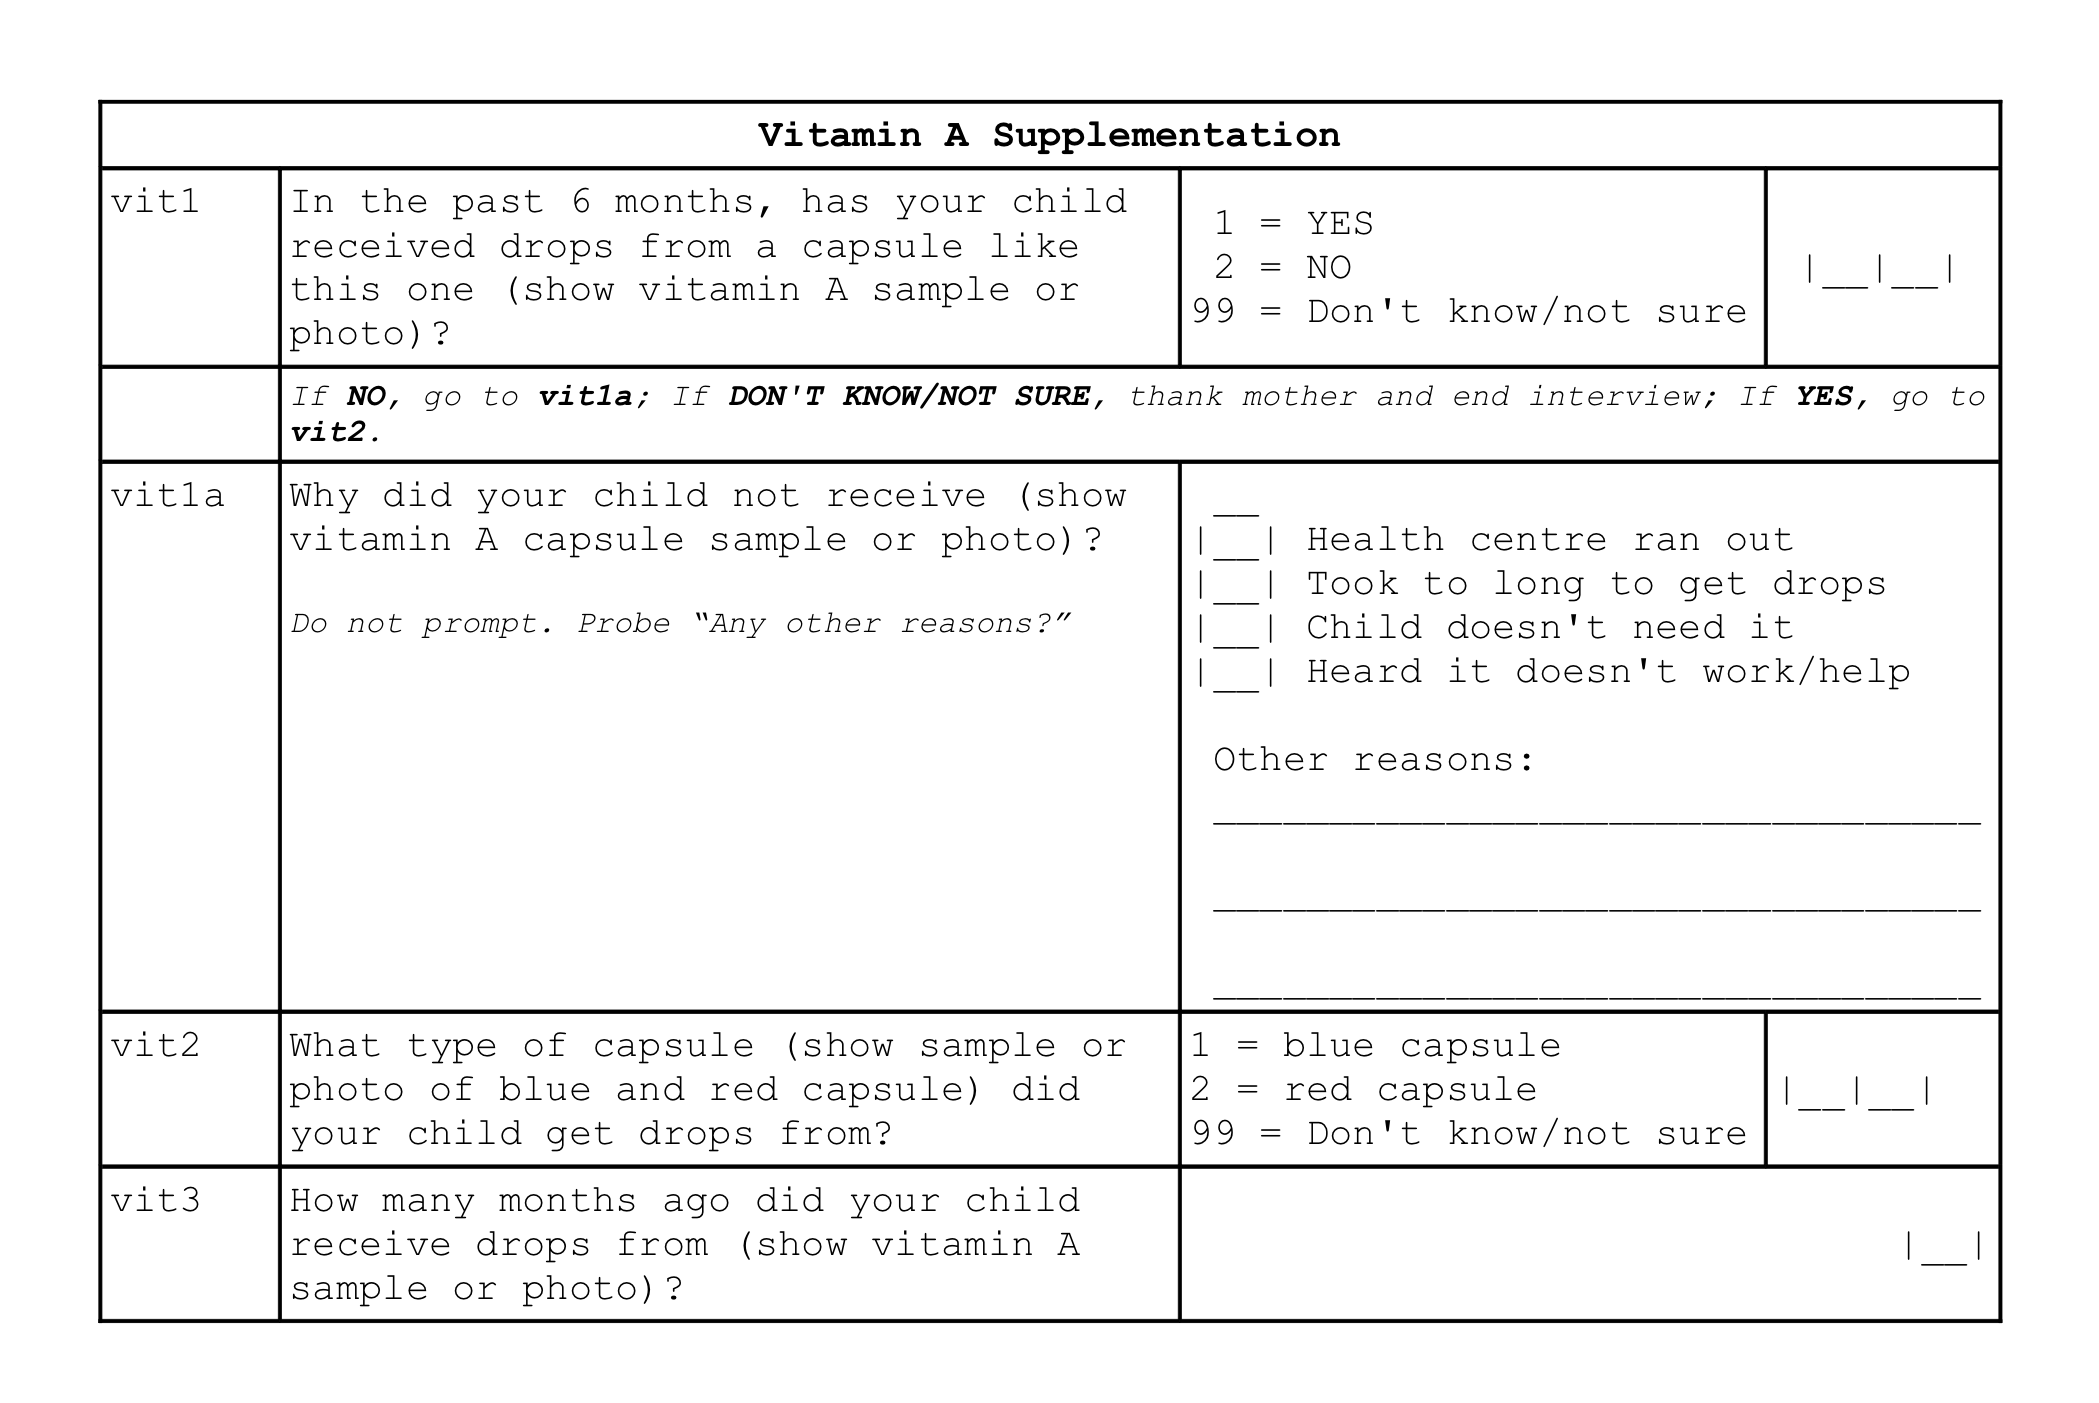
\includegraphics[width=0.9\linewidth]{forms/childForm4} 

}

\caption{Children 6-59 months old and their mothers survey sample/template form}\label{fig:childform1}
\end{figure}

\hypertarget{using-open-data-kit}{%
\section{Using Open Data Kit}\label{using-open-data-kit}}

Based on the template forms described in the previous sections, a
digital data collection system using Open Data Kit (ODK) has been
developed. These forms are availabe as a
\href{https://github.com/validmeasures/liberiaS3Mforms}{Github
repository}. The system is composed of two forms.

\hypertarget{village-form}{%
\subsection{Village form}\label{village-form}}

This form (\texttt{liberiaCoverageVillageForm.xlsx} and
\texttt{liberiaCoverageVillageForm.xml}) collects information on the
villages or primary sampling units (PSU) selected for the Liberia
Coverage Survey. This information includes:

\begin{enumerate}
\def\labelenumi{\arabic{enumi}.}
\item
  County name (and identifier)
\item
  Village name (and identifier)
\item
  Village population size
\item
  Village geocoordinates
\end{enumerate}

\hypertarget{coverage-form}{%
\subsection{Coverage form}\label{coverage-form}}

This form (\texttt{liberiaCoverage.xlsx} and
\texttt{liberiaCoverage.xml}) collects information on the various
coverage indicators assessed in the Liberia Coverage Survey:

\begin{enumerate}
\def\labelenumi{\arabic{enumi}.}
\item
  CMAM coverage
\item
  Iron-folic acid supplementation coverage
\item
  IYCF counselling coverage
\item
  Micronutrient powder supplementation coverage
\item
  Vitamin A supplementation coverage
\end{enumerate}

The coverage form has been developed in such a way that it implements
the survey as per survey design such that the modules for IFA coverage,
IYCF counselling coverage, MNP supplementation coverage and vitamin A
supplementation coverage are only shown based on the sampling interval
for a particular primary sampling unit (PSU) and based on the different
eligibitlity requirements for each coverage survey module.

\hypertarget{usage}{%
\subsection{Usage}\label{usage}}

For those wanting to test out the forms on their own Android mobile
devices, the following applications need to be downloaded and installed
from the Google Play Store:

\begin{itemize}
\item
  ODK Collect
  (\href{https://play.google.com/store/apps/details?id=org.odk.collect.android\&hl=en_GB}{link})
\item
  ODK Counter
  (\href{https://play.google.com/store/apps/details?id=org.opendatakit.counter\&hl=en_GB}{link})
\end{itemize}

Once these applications are isntalled, there are two option for getting
the Liberia Coverage Survey forms onto mobile devices.

\hypertarget{using-odk-aggregator-or-other-similar-odk-servers}{%
\subsection{1. Using ODK Aggregator or other similar ODK
servers}\label{using-odk-aggregator-or-other-similar-odk-servers}}

The XLSForm can be uploaded to a remote server-based ODK Aggregator or
other ODK servers such as ONA, SurveyCTO, KoBoToolbox and the like. The
form is validated and then converted into XML format which can then be
retrieved from the server into mobile devices as blank forms.

For the purposes of viewing and testing the Liberia Coverage Survey
forms, a test server has been setup. To view and/or test the Liberia
Coverage Survey forms, ODK Collect in the mobile devices will need to be
connected to the server. This is described
\href{https://docs.opendatakit.org/collect-connect-aggregate/}{here}.
The following ODK Aggregate server setttings should be used:

~

\textbf{url}: \url{https://odk.ona.io}

\textbf{username:} validtrial

\textbf{password:} zEF-STN-5ze-qom

~

Once ODK Collect has been connected to the test server, it will now be
possible to pull the Liberia Coverage Survey forms into ODK Collect in
the mobile device using the instructions found
\href{https://docs.opendatakit.org/collect-forms/}{here}.

Once the Liberia Coverage Survey forms have been pulled into the ODK
Collect in the mobile device, the forms can be viewed and tested by
following the instructions
\href{https://docs.opendatakit.org/collect-filling-forms/}{here}.

\hypertarget{convert-to-xml-and-transfer-to-mobile-devices-via-usb-cable-connection}{%
\subsection{2. Convert to XML and transfer to mobile devices via USB
cable
connection}\label{convert-to-xml-and-transfer-to-mobile-devices-via-usb-cable-connection}}

The XML version of this form can then be transferred to the mobile
devices (into the device's \texttt{odk} folder) via local USB
connection. This can be done by following the instructions
\href{https://docs.opendatakit.org/collect-forms/\#loading-forms-directly}{here}.
The associated media files for the forms (found in the folder called
\texttt{media} in this repository) will also need to be transferred to
the mobile device. This can be done by following the instructions
\href{https://docs.opendatakit.org/collect-forms/\#loading-form-media}{here}.

\hypertarget{data}{%
\chapter{Data management and analysis}\label{data}}

Data will be collected using an electronic data entry system based on
the \textbf{Open Data Kit (ODK)} standard that runs on the Android®
operating software (OS) platform for mobile devices. The study
instrument (see Section \ref{questionnaire}) will be encoded into the
electronic data entry system platform and will be served out of either a
local computer server or a remote/cloud-based server\footnote{This will
  depend on what resources are available to the Liberia Institute of
  Statistics and Geo-Information Services. Valid International has
  resources to implement either a local server or a remote server
  solution.}. Each study team will be provided with mobile devices
running on Android® OS that have been configured with an application
that will receive the electronic data form. All measurements and answers
by respondents will then be recorded on the mobile devices and will then
be transmitted to the local server or the remote server whenever there
is a mobile phone and / or WiFi signal.

Appropriate data check mechanisms will be put in place using the data
check systems available with the ODK system. Spot checks by study
supervisor/s will be done in the field to ensure that enumerators are
performing the measurements correctly, administering the study
instrument correctly and entering all data accordingly. Further checks
will be performed by the survey manager on the data as needed as they
are received by the local server or remote server.

The digital data collection forms based on the Open Data Kit (ODK)
standard using XLSform and XML is available at
\url{https://github.com/validmeasures/liberiaS3Mforms}. The form
faithfully replicates the paper-based forms described in Section
\ref{questionnaire}. The form also faithfully replicates the sampling
design described by the survey design such that proposed sampling
interval within a primary sampling unit (PSU) is implemented as the
survey team goes house-to-house finding SAM cases. The modules on IFA
supplementation, IYCF counselling, vitamin A supplementation and MNP
supplementation coverage appear appropriately on the digital forms when
the correct household based on the sampling interval is being
interviewed. The forms also appear appropriately based on eligibility of
the child/mother as respnodents to the specific survey modules.

These forms can be viewed and tested using an Android-based mobile
device. Instructions for usage can be found at
\url{https://github.com/validmeasures/liberiaS3Mforms}.

Data analysis will be done using R language for statistical computing
\citep{R:2018} through bespoke analytic scripts put together into
application-based workflow which can be used by non-R users. The
application that will be created for this study will be designed such
that an automatic reporting format is produced including maps, figures
and tables of results.

\hypertarget{analytical-approach-for-estimating-coverage-indicators}{%
\section{Analytical approach for estimating coverage
indicators}\label{analytical-approach-for-estimating-coverage-indicators}}

It is important to note that data analysis procedures need to account
for the sample design. All major statistical analysis software can do
this (details vary). There are two things to note:

\begin{itemize}
\tightlist
\item
  This survey is a two-stage sample. Subjects are sampled from a small
  number of primary sampling units (PSUs).
\item
  This survey is \textbf{not} prior weighted. This means that per-PSU
  sampling weights will be needed. These are usually the populations of
  the PSU.
\end{itemize}

This sample design will need to be specified to your statistical
analysis software. Failing this, the analysis may produce estimates that
place undue weight to observations from smaller communities with
confidence intervals with lower than nominal coverage (i.e.~they will be
too narrow).

For this survey, the \emph{blocked weighted bootstrap} estimation
approach will be used:

\begin{itemize}
\tightlist
\item
  \textbf{Blocked} : The block corresponds to the PSU or cluster.
\item
  \textbf{Weighted} : The sampling procedure for this survey does not
  use population proportional sampling to weight the sample prior to
  data collection as is done with SMART type surveys. This means that a
  posterior weighting procedure is required. The ``roulette wheel''
  algorithm to weight (i.e.~by population) the selection probability of
  PSUs in bootstrap replicates will be utilised.
\end{itemize}

A total of \texttt{m} PSUs are sampled \emph{with-replacement} from the
survey dataset where \texttt{m} is the number of PSUs in the survey
sample. Individual records within each PSU are then sampled
\emph{with-replacement}. A total of n' records are sampled
\emph{with-replacement} from each of the selected PSUs where \texttt{n}
is the number of individual records in a selected PSU. The resulting
collection of records replicates the original survey in terms of both
sample design and sample size. A large number of replicate surveys are
taken (minimum of \(r = 399\) replicate surveys but this can be
changed). The required statistic (e.g.~the mean of an indicator value)
is applied to each replicate survey. The reported estimate consists of
the 50th (point estimate), 2.5th (lower 95\% confidence limit), and the
97.5th (upper 95\% confidence limit) percentiles of the distribution of
the statistic observed across all replicate surveys. The blocked
weighted bootstrap procedure is outlined in Figure
\ref{fig:indicators31}.

The principal advantages of using a bootstrap estimator are:

\begin{itemize}
\item
  Bootstrap estimators work well with small sample sizes.
\item
  The method is \emph{non-parametric} and uses empirical rather than
  theoretical distributions. There are no assumptions of things like
  normality to worry about.
\item
  The method allows estimation of the sampling distribution of almost
  any statistic using only simple computational methods.
\end{itemize}

\newpage

\begin{figure}[H]

{\centering 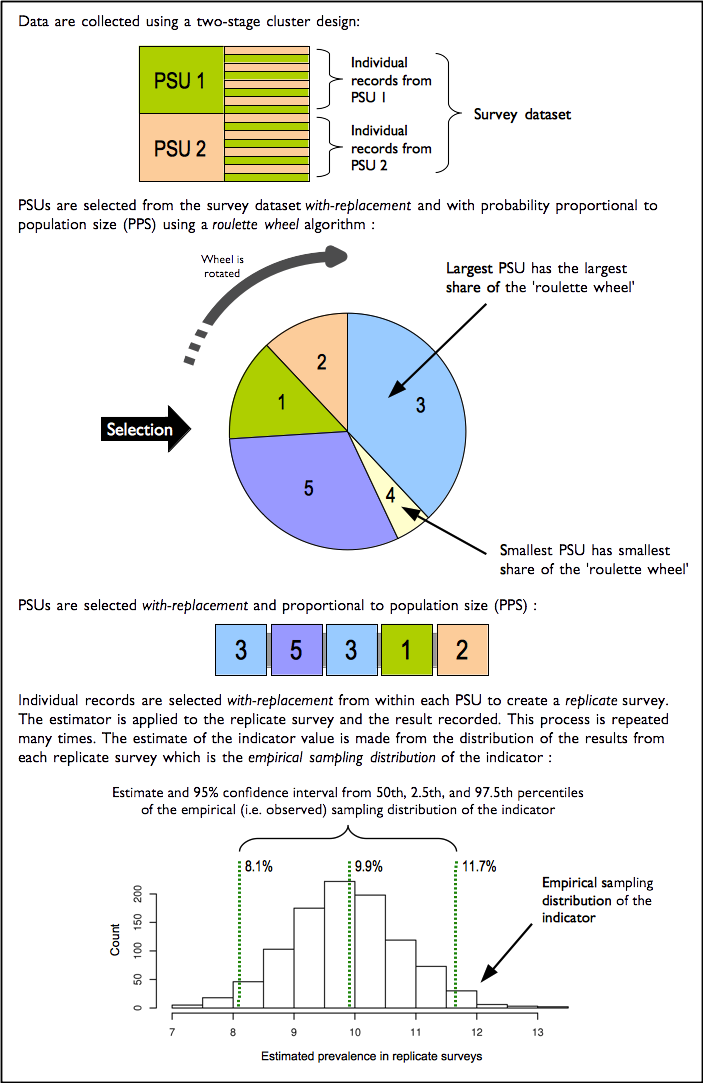
\includegraphics[width=9.76in]{figures/bbw} 

}

\caption{The blocked weighted bootstrap}\label{fig:indicators31}
\end{figure}

\hypertarget{analytical-approach-for-mapping-coverage-indicators}{%
\section{Analytical approach for mapping coverage
indicators}\label{analytical-approach-for-mapping-coverage-indicators}}

The indicator mapping will create a surface map of indicator values
using spatial interpolation. There are various approaches and methods of
spatial interpolation, the main differences are determined by the
weights applied to the point dataset to estimate values at each of the
unknown points of the surface map. For the Liberia coverage survey,
spatial interpolation will be performed using the inverse distance
weighting (IDW) method. As the name implies, the IDW method uses weights
that are inversely proportional to the distance of a point being
estimated from the sampling point locations
\citep{isaaks1989applied, diggle2007mbg, diggle2013statistical}. This
can be mathematically demonstrated as follows:

~

\[\begin{aligned}
\hat{v} & ~ = ~ \frac{\displaystyle \sum\limits_{i = 1}^{n} \frac{1}{d_{i}^{p}}v_{i}}{\displaystyle \sum\limits_{i = 1}^{n}\frac{1}{d_{i}^{p}}} \\
\\
where: & \\
\\
d_1 \ldots d_n & ~ = ~ \text{distances from each } n \text{ sampling points to estimation point} \\
p & ~ = ~ \text{power of the distance} \\
v_1 \ldots v_n & ~ = ~ \text{sample values}
\end{aligned}\]

~

The power of the distance \texttt{p} is an important aspect of the IDW
method for point estimation. The influence of \texttt{p} to the weights
applied to the point estimation is such that as \texttt{p} approaches 0,
the weights become more similar, thereby giving more weight to the
nearest sample values. As \texttt{p} approaches \(\infty\), the weights
become more different from each other, thereby giving more weight to the
closest sample. The power of the distance \texttt{p} has been
traditionally set at 2 for convenience and ease of calculations. In
theory, given a set \texttt{p}, IDW calculations can be performed using
manual calculations aided by a spreadsheet and / or a calculator as it
requires fewer calculations. For the Liberia Coverage Survey, \texttt{p}
will be initially set at 2 and then cross-validation (see below) will be
applied to optimise \texttt{p} to a value that minimises the estimation
errors at each of the sampling point locations.

Cross-validation is a technique applied to validate predictive models.
It assesses how accurately the predictive model performs in practice.
IDW is one of the simplest model-based interpolation methods available,
but ideally would still require a form of cross-validation to determine
the optimal value of the distance power \texttt{p} (described above).

A two-fold cross validation \citep{bivand2008applied} in which data
points are randomly split into two sets of equal size, with one set
assigned as the validation data for testing the model, and the other set
as the training data. The validation data is then interpolated using the
IDW method with an initial \texttt{p} of 2 and the resulting predictions
were compared with the training data. Comparison is made using the sum
of the squared residuals between the predicted values and the observed
values to report errors. Optimisation is then performed by replicating
the two-fold cross validation process 100 times using randomly generated
values for \texttt{p}. Out of these replicates, the value of \texttt{p}
that provided prediction results with the minimum errors is selected as
the distance power for the eventual interpolation performed.

\hypertarget{standard}{%
\chapter{Anthropometric measurement standardisation
test}\label{standard}}

The survey personnel should go through theoretical discussions and
demonstrations on how to perform the anthropometric measurements. This
should then be followed by practical demonstration of the measurement
techniques, measurement readings and recording ideally with a large
number of children particularly if there is a large number of survey
personnel. Once all personnel have had the opportunity to adequately
practice their measurement and recording techniques, a standardisation
test or exercise must be carried out. Chapter \ref{standard} provides
detailed instructions on how to carry out an anthropometric measurement
standardisation test as part of a training process in preparation for a
nutrition survey.

\hypertarget{objectives}{%
\section{Objectives}\label{objectives}}

The standardisation test evaluates the \textbf{precision} and the
\textbf{accuracy} of the measurements taken by each survey personnel.

The \textbf{accuracy} of measurements taken by survey personnel is
determined by how close they are to the true value with repeated
measurements. On the other hand, the \textbf{precision} of measurements
taken by survey personnel is determined by how similar the values are of
repeated measurements made. In preparation for a nutrition survey while
the survey personnel are in training, the aim is for survey personnel to
be \emph{highly accurate} and \emph{highly precise} with their
anthropometric measurements.

\begin{figure}

{\centering 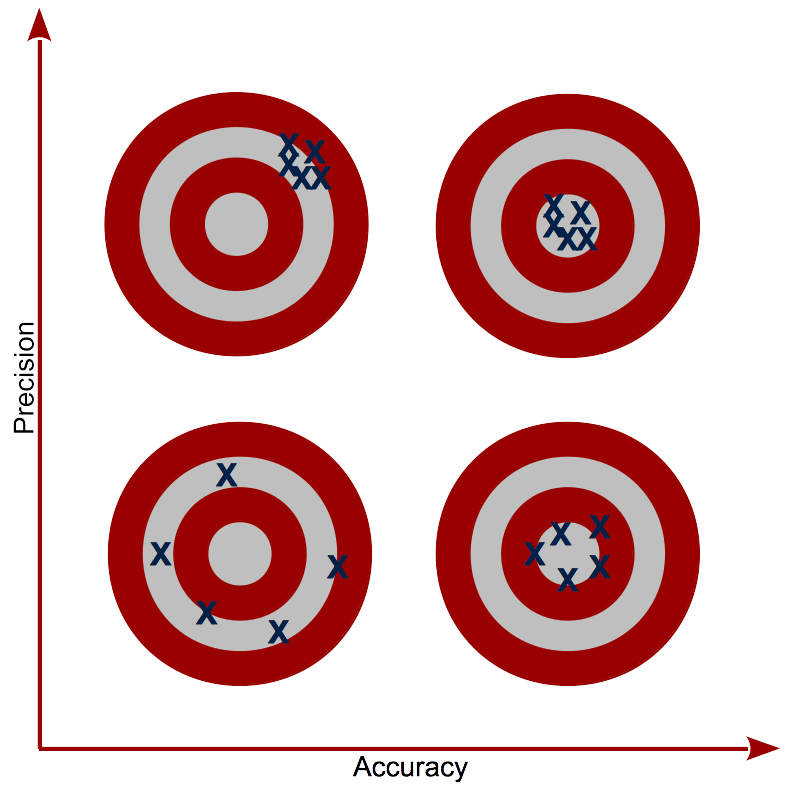
\includegraphics[width=11.11in]{figures/accuracyPrecision} 

}

\caption{Relationship between accuracy and precision}\label{fig:standard01}
\end{figure}

\hypertarget{mechanics}{%
\section{Mechanics}\label{mechanics}}

The general process of the standardisation test is for each survey
personnel to take measurements of at least 10 children 6-59 months,
twice, with an interval of time between the 1st and 2nd measurements.

\hypertarget{test-parameters}{%
\subsection{Test parameters}\label{test-parameters}}

The following test parameters need to be followed when conducting an
anthropometric standardisation test:

\begin{enumerate}
\def\labelenumi{\arabic{enumi}.}
\item
  The same type of equipment must be used both during the
  standardisation test and the survey
\item
  Each child is measured with the same equipment
\item
  The supervisor must observe how measurements are being taken
\item
  Survey personnel measurements are compared to the reference
  (supervisor) values
\item
  Survey personnel measurements are compared to the repeated measures
  taken (intra-observer)
\end{enumerate}

\hypertarget{test-organisation-and-requirements}{%
\subsection{Test organisation and
requirements}\label{test-organisation-and-requirements}}

The following test organisation and requirements need to be met in order
to conduct a credible standardisation test:

\begin{enumerate}
\def\labelenumi{\arabic{enumi}.}
\item
  Spacious and shady area
\item
  Healthy children between 6 and 59 months or according to the age group
  targeted by the survey
\item
  Incentives provided for the mother and children
\item
  Survey personnel are grouped into pairs, but each personnel will carry
  out the measurements in turn
\item
  There should only be one pair of survey personnel per child at any
  time during the test
\item
  Each survey personnel is given a unique ID. For example if there are
  20 survey personnel, a unique ID from 1 to 20 is given to each survey
  personnel. The supervisor's ID is always 0
\item
  Each measurement station should have a height board, weighing scale
  and a MUAC tape
\item
  Each child must remain with their mother in a fixed station with a
  unique ID number. For example if there are 10 mother and children
  pairs, a unique ID from 1 to 10 is given to each pair
\item
  It is not allowed for pairs of survey personnel to speak with other
  pairs during the test
\end{enumerate}

\hypertarget{timeframe}{%
\subsection{Timeframe}\label{timeframe}}

In order to follow the test parameters specified above and organise the
test appropriately, a considerable amount of time needs to be set aside
for conducting the test.

For a survey team of about 20 survey personnel, the test can be carried
out in 2 half-days such that half of the survey personnel (first half of
each team) measures 10 children in the morning and the other half
(second half of each team) measures the same 10 children in the
afternoon.

It would be possible to have a different set of 10 children for the
afternoon session. However, the results of the first half who took the
test in the morning cannot be combined with the results of the second
half who took the test in the afternoon.

For larger scale surveys with survey personnel more than 20, more days
will be required to conduct the test to appropriately and to correct
specifications.

\hypertarget{steps-in-carrying-out-the-standardisation-test}{%
\subsection{Steps in carrying out the standardisation
test}\label{steps-in-carrying-out-the-standardisation-test}}

\begin{enumerate}
\def\labelenumi{\arabic{enumi}.}
\tightlist
\item
  The supervisor carefully performs the measurements on each child
  without allowing the teams to see the values. The supervisor records
  his/her measurements on the standardisation test form for the first
  round of measurements.
\end{enumerate}

Standardisation Test Form - Measurement Round 1

Enumerator ID: \_\_\_\_\_ ~ ~ ~ Enumerator Name:
\_\_\_\_\_\_\_\_\_\_\_\_\_\_\_\_\_\_\_

\begin{longtable}[]{@{}lllll@{}}
\toprule
\begin{minipage}[b]{0.17\columnwidth}\raggedright
Child ID\strut
\end{minipage} & \begin{minipage}[b]{0.17\columnwidth}\raggedright
Weight (kg)\strut
\end{minipage} & \begin{minipage}[b]{0.17\columnwidth}\raggedright
Height (cm)\strut
\end{minipage} & \begin{minipage}[b]{0.17\columnwidth}\raggedright
MUAC (mm)\strut
\end{minipage} & \begin{minipage}[b]{0.17\columnwidth}\raggedright
Oedema (yes/no)\strut
\end{minipage}\tabularnewline
\midrule
\endhead
\begin{minipage}[t]{0.17\columnwidth}\raggedright
01\strut
\end{minipage} & \begin{minipage}[t]{0.17\columnwidth}\raggedright
\strut
\end{minipage} & \begin{minipage}[t]{0.17\columnwidth}\raggedright
\strut
\end{minipage} & \begin{minipage}[t]{0.17\columnwidth}\raggedright
\strut
\end{minipage} & \begin{minipage}[t]{0.17\columnwidth}\raggedright
\strut
\end{minipage}\tabularnewline
\begin{minipage}[t]{0.17\columnwidth}\raggedright
02\strut
\end{minipage} & \begin{minipage}[t]{0.17\columnwidth}\raggedright
\strut
\end{minipage} & \begin{minipage}[t]{0.17\columnwidth}\raggedright
\strut
\end{minipage} & \begin{minipage}[t]{0.17\columnwidth}\raggedright
\strut
\end{minipage} & \begin{minipage}[t]{0.17\columnwidth}\raggedright
\strut
\end{minipage}\tabularnewline
\begin{minipage}[t]{0.17\columnwidth}\raggedright
03\strut
\end{minipage} & \begin{minipage}[t]{0.17\columnwidth}\raggedright
\strut
\end{minipage} & \begin{minipage}[t]{0.17\columnwidth}\raggedright
\strut
\end{minipage} & \begin{minipage}[t]{0.17\columnwidth}\raggedright
\strut
\end{minipage} & \begin{minipage}[t]{0.17\columnwidth}\raggedright
\strut
\end{minipage}\tabularnewline
\begin{minipage}[t]{0.17\columnwidth}\raggedright
04\strut
\end{minipage} & \begin{minipage}[t]{0.17\columnwidth}\raggedright
\strut
\end{minipage} & \begin{minipage}[t]{0.17\columnwidth}\raggedright
\strut
\end{minipage} & \begin{minipage}[t]{0.17\columnwidth}\raggedright
\strut
\end{minipage} & \begin{minipage}[t]{0.17\columnwidth}\raggedright
\strut
\end{minipage}\tabularnewline
\begin{minipage}[t]{0.17\columnwidth}\raggedright
05\strut
\end{minipage} & \begin{minipage}[t]{0.17\columnwidth}\raggedright
\strut
\end{minipage} & \begin{minipage}[t]{0.17\columnwidth}\raggedright
\strut
\end{minipage} & \begin{minipage}[t]{0.17\columnwidth}\raggedright
\strut
\end{minipage} & \begin{minipage}[t]{0.17\columnwidth}\raggedright
\strut
\end{minipage}\tabularnewline
\begin{minipage}[t]{0.17\columnwidth}\raggedright
06\strut
\end{minipage} & \begin{minipage}[t]{0.17\columnwidth}\raggedright
\strut
\end{minipage} & \begin{minipage}[t]{0.17\columnwidth}\raggedright
\strut
\end{minipage} & \begin{minipage}[t]{0.17\columnwidth}\raggedright
\strut
\end{minipage} & \begin{minipage}[t]{0.17\columnwidth}\raggedright
\strut
\end{minipage}\tabularnewline
\begin{minipage}[t]{0.17\columnwidth}\raggedright
07\strut
\end{minipage} & \begin{minipage}[t]{0.17\columnwidth}\raggedright
\strut
\end{minipage} & \begin{minipage}[t]{0.17\columnwidth}\raggedright
\strut
\end{minipage} & \begin{minipage}[t]{0.17\columnwidth}\raggedright
\strut
\end{minipage} & \begin{minipage}[t]{0.17\columnwidth}\raggedright
\strut
\end{minipage}\tabularnewline
\begin{minipage}[t]{0.17\columnwidth}\raggedright
08\strut
\end{minipage} & \begin{minipage}[t]{0.17\columnwidth}\raggedright
\strut
\end{minipage} & \begin{minipage}[t]{0.17\columnwidth}\raggedright
\strut
\end{minipage} & \begin{minipage}[t]{0.17\columnwidth}\raggedright
\strut
\end{minipage} & \begin{minipage}[t]{0.17\columnwidth}\raggedright
\strut
\end{minipage}\tabularnewline
\begin{minipage}[t]{0.17\columnwidth}\raggedright
09\strut
\end{minipage} & \begin{minipage}[t]{0.17\columnwidth}\raggedright
\strut
\end{minipage} & \begin{minipage}[t]{0.17\columnwidth}\raggedright
\strut
\end{minipage} & \begin{minipage}[t]{0.17\columnwidth}\raggedright
\strut
\end{minipage} & \begin{minipage}[t]{0.17\columnwidth}\raggedright
\strut
\end{minipage}\tabularnewline
\begin{minipage}[t]{0.17\columnwidth}\raggedright
10\strut
\end{minipage} & \begin{minipage}[t]{0.17\columnwidth}\raggedright
\strut
\end{minipage} & \begin{minipage}[t]{0.17\columnwidth}\raggedright
\strut
\end{minipage} & \begin{minipage}[t]{0.17\columnwidth}\raggedright
\strut
\end{minipage} & \begin{minipage}[t]{0.17\columnwidth}\raggedright
\strut
\end{minipage}\tabularnewline
\bottomrule
\end{longtable}

\BeginKnitrBlock{rmddownload}
Download the standardisation test form
\href{forms/standardForm.pdf}{here}.
\EndKnitrBlock{rmddownload}

\begin{enumerate}
\def\labelenumi{\arabic{enumi}.}
\setcounter{enumi}{1}
\item
  Each team starts with a different child, and the first half of the
  team measures the child once and records the results in a standard
  form for the 1st measurement (as above). The current measurer should
  make sure that he/she is entering data in the row corresponding to the
  child ID of the child he/she is currently measuring.
\item
  When the first half of the team has done the measurements for the
  current child, they should move on to the next child. After the first
  half of all the teams has measured 10 children once, the first
  measurement round forms are handed in. The teams and the children then
  take a break. Appropriate incentives including food and drinks to
  snack on during the break should be provided to the mothers and
  children.
\item
  After the break, the first half of the team repeats the whole process
  and measures each child for the second time and records his/her
  measurements onto the standardisation test form for the second round
  of measurements. After the the first half of all the teams has
  measured 10 children twice, the second measurement round forms are
  handed in. The teams and the children then take a break for lunch (end
  of first half of the day/first half of the test). Appropriate lunch
  arrangements should be prepared for the mothers and children.
\item
  After the lunch break or on a new day altogether, the whole process is
  done all over again but this time, the second half of the teams will
  be performing the measurements. Ideally, the same set of mother and
  child pairs should be utilised for the second half day of testing.
  However, it may be that some of the mothers will be unable to come
  back to help. If for the second half day of testing the mother and
  child pairs are different from the first half day, then measurements
  made in the second half day cannot be mixed with the data from the
  first half day when reporting on the performance in the
  standardisation test of the survey personnel.
\end{enumerate}

\bibliography{book.bib}


\end{document}
